\documentclass[12pt,a4paper,twoside]{book}
\usepackage{graphicx}
\usepackage{setspace}
\usepackage[utf8]{inputenc}
\usepackage[english]{babel}
\usepackage{natbib}
\usepackage{color}
\usepackage{multirow}
\usepackage{subfigure}
\usepackage{acronym}
\usepackage{hyperref}
\usepackage[capitalise]{cleveref}
\usepackage{amsmath,amsmath,amssymb} 
\usepackage{fancyhdr}
\usepackage{epsfig, amsmath}
\usepackage{algorithm}
\usepackage{algorithmic}
\usepackage{longtable}
\usepackage{booktabs}
\usepackage{array}
\usepackage[width=.9\textwidth]{caption}
\usepackage{svg}
\usepackage[T1]{fontenc}
\usepackage{titlesec}
\graphicspath{ {images/} }

% general settings

% cleverref settings
\crefformat{section}{\S#2#1#3} 
\crefformat{subsection}{\S#2#1#3}
\crefformat{subsubsection}{\S#2#1#3}

\hypersetup{
	linktocpage=true,
	colorlinks=true,
	linkcolor=blue,
	citecolor=blue,
}
\definecolor{Hgray}{gray}{0.6}

\newenvironment{definition}[1][Definition]{\begin{trivlist}
\item[\hskip \labelsep {\bfseries #1}]}{\end{trivlist}}

\setlength{\topmargin}{0cm}
\setlength{\textheight}{23cm}
\setlength{\textwidth}{17cm}
\setlength{\oddsidemargin}{0cm}
\setlength{\evensidemargin}{0cm}
\setlength{\headheight}{1cm}

% Set numbered 'sub-sub-sections' and appear in the TOC
\setcounter{secnumdepth}{3}
\setcounter{tocdepth}{2}

% settings for code
\renewcommand{\algorithmicrequire}{\textbf{Input: }}
\renewcommand{\algorithmicensure}{\textbf{Output: }}

% settings for array stretching in tables
% \renewcommand\arraystretch{1.25}

% adding more subsectioning options
\titleclass{\subsubsubsection}{straight}[\subsection]

\newcounter{subsubsubsection}[subsubsection]
\renewcommand\thesubsubsubsection{\thesubsubsection.\arabic{subsubsubsection}}
\renewcommand\theparagraph{\thesubsubsubsection.\arabic{paragraph}} % optional; useful if paragraphs are to be numbered

\titleformat{\subsubsubsection}
  {\normalfont\normalsize\bfseries}{\thesubsubsubsection}{1em}{}
\titlespacing*{\subsubsubsection}
{0pt}{3.25ex plus 1ex minus .2ex}{1.5ex plus .2ex}

\makeatletter
\renewcommand\paragraph{\@startsection{paragraph}{5}{\z@}%
  {3.25ex \@plus1ex \@minus.2ex}%
  {-1em}%
  {\normalfont\normalsize\bfseries}}
\renewcommand\subparagraph{\@startsection{subparagraph}{6}{\parindent}%
  {3.25ex \@plus1ex \@minus .2ex}%
  {-1em}%
  {\normalfont\normalsize\bfseries}}
\def\toclevel@subsubsubsection{4}
\def\toclevel@paragraph{5}
\def\toclevel@paragraph{6}
\def\l@subsubsubsection{\@dottedtocline{4}{7em}{4em}}
\def\l@paragraph{\@dottedtocline{5}{10em}{5em}}
\def\l@subparagraph{\@dottedtocline{6}{14em}{6em}}
\makeatother

\setcounter{secnumdepth}{4}
\setcounter{tocdepth}{4}

%%%%%%%%%%%%
% DOCUMENT %
%%%%%%%%%%%%
\begin{document}

% portada
\newpage
\thispagestyle{empty}

\baselineskip 2em

%\vspace*{1cm}

\centerline{
\includegraphics[width=0.6\textwidth]{ch0/UOC-logo}}
\begin{center}
\textsc{Universitat Oberta de Catalunya (UOC) \\
 Máster Universitario en Ciencia de Datos (\textit{Data Science})\\}

%\centerline {\pic{UOC}{4cm}}

\vspace*{1.5cm}

\textsc{\Large TRABAJO FINAL DE MÁSTER}

\vspace*{0.5cm}

\textsc{\large Área: Big Data / Machine Learning}


%\textbf{\Huge VirtualTechLab Model: }

\vspace*{2.0cm}

\textbf{\Large Automatic image descriptions}

\textbf{\large A deep-learning approach}

\vspace{2.5cm}
\baselineskip 1em

\baselineskip 2em
-----------------------------------------------------------------------------\\
Autor:      Mario Gómez Martínez\\
Tutor:      Anna Bosch Rué\\
Profesor:   Jordi Casas Roma\\
-----------------------------------------------------------------------------\\
\vspace*{1.5cm}
Valencia, \today

\end{center}

\newpage
\pagestyle{empty}
\hfill

\newpage
% abstract
\pagenumbering{roman} 
\setcounter{page}{1} 
\pagestyle{plain}

%%%%%%%%%%%%%%%%
%%% CREDITOS %%%
%%%%%%%%%%%%%%%%
\chapter*{Copyright}

\vspace{1cm}

\begin{figure}[ht]
    \centering
	
\includegraphics[scale=1]{ch0/license.png}
\end{figure}

This work is licensed under \href{https://creativecommons.org/licenses/by-nc-sa/3.0/es/deed.en}{Creative Commons Attribution-NonCommercial-ShareAlike 4.0 Spain License (CC BY-NC-SA 4.0 ES)} 

\vspace{1cm}

\begin{figure}[ht]
    \centering
	
\includegraphics[scale=1]{ch0/licencia.png}
\end{figure}

Esta obra está sujeta a una licencia de \href{https://creativecommons.org/licenses/by-nc-sa/4.0/es/}{Reconocimiento-NoComercial-CompartirIgual 4.0 España de Creative Commons (CC BY-NC-SA 4.0 ES)}


%%%%%%%%%%%%%
%%% FICHA %%%
%%%%%%%%%%%%%
\chapter*{FICHA DEL TRABAJO FINAL}

\begin{table}[ht]
	\centering{}
	\renewcommand{\arraystretch}{2}
	\begin{tabular}{r | l}
		\hline
		Título del trabajo: & Automated generation of image captions\\
		\hline
        Nombre del autor: & Mario Gómez Martínez\\
		\hline
        Nombre del colaborador/a docente: & Anna Bosch Rué\\
		\hline
        Nombre del PRA: & Jordi Casas Roma\\
		\hline
        Fecha de entrega (mm/aaaa): & 06/2019\\
		\hline
        Titulación o programa: & Máster en Ciencia de Datos\\
		\hline
        Área del Trabajo Final: & Aprendizaje automático\\
		\hline
        Idioma del trabajo: & Inglés\\
		\hline
        Palabras clave & Aprendizaje Profundo, Descripción de Imágenes\\
		\hline
	\end{tabular}
\end{table}

%%%%%%%%%%%%%%%%%%%
%%% DEDICATORIA %%%
%%%%%%%%%%%%%%%%%%%
\chapter*{Dedicatoria}

Dedicado a mi compañera, siempre ahí, para lo bueno y para lo malo, cercana, constante, inspiradora...

%%%%%%%%%%%%%%%%%%%
%%% Agradecimientos %%%
%%%%%%%%%%%%%%%%%%%
% \chapter*{Agradecimientos}

% Quisiera agradecer a...

%%%%%%%%%%%%%%%%
%%% RESUMEN  %%%
%%%%%%%%%%%%%%%%
\chapter*{Abstract}
\addcontentsline{toc}{chapter}{Abstract}

\onehalfspacing

Automatic image captioning, the task of automatically producing a natural-language description for an image, has the potential to assist those with visual impairments by explaining images using text-to-speech systems. However, accurate image captioning is a challenging task that requires integrating and pushing further the latest improvements at the intersection of computer vision and natural language processing fields

This work aims at building an advanced model based on neural networks and deep learning for the automated generation of image captions. 


\vspace{1.5cm}

\textbf{Keywords}: Deep Learning, Artificial Neural Networks, Automated image captioning


\chapter*{Resumen}
\addcontentsline{toc}{chapter}{Resumen}

\onehalfspacing

El subtitulado automático de imágenes, la tarea de producir automáticamente una descripción en lenguaje natural para una imagen, tiene el potencial de ayudar a las personas con discapacidades visuales a explicar las imágenes mediante sistemas de conversión de texto a voz. Sin embargo, el subtitulado preciso de imágenes es una tarea desafiante que requiere integrar y avanzar en la intersección de los campos de procesamiento de lenguaje natural y visión por computador.

Este trabajo pretende desarrollar un modelo basado en redes neuronales y aprendizaje profundo para la generación automática de descripciones de imágenes.


\vspace{1.5cm}

\textbf{Palabras clave}: Aprendizaje Profundo, Redes Neuronales Artificiales, Descripción automática de imágenes
\newpage

\pagestyle{fancy}
\renewcommand{\chaptermark}[1]{ \markboth{#1}{}}
\renewcommand{\sectionmark}[1]{\markright{ \thesection.\ #1}}
\lhead[\fancyplain{}{\bfseries\thepage}]{\fancyplain{}{\bfseries\rightmark}}
\rhead[\fancyplain{}{\bfseries\leftmark}]{\fancyplain{}{\bfseries\thepage}}
\cfoot{}

% indice
\cleardoublepage
\phantomsection
\addcontentsline{toc}{chapter}{Index}
\tableofcontents
% listado de figuras
\cleardoublepage
\phantomsection
\addcontentsline{toc}{chapter}{List of Figures}
\listoffigures
% listado de tablas
\cleardoublepage
\phantomsection
\addcontentsline{toc}{chapter}{List of Tables}
\listoftables

\thispagestyle{empty}

\pagenumbering{arabic}

\pagestyle{fancy}
\renewcommand{\chaptermark}[1]{ \markboth{#1}{}}
\renewcommand{\sectionmark}[1]{\markright{ \thesection.\ #1}}
\lhead[\fancyplain{}{\bfseries\thepage}]{\fancyplain{}{\bfseries\rightmark}}
\rhead[\fancyplain{}{\bfseries\leftmark}]{\fancyplain{}{\bfseries\thepage}}
\cfoot{}

\onehalfspacing

% capitulos del documento
\chapter{Introduction}
\label{chapter:introduccion}

\section{Motivation}

The web provides a vast amount of information, including a lot of text, but it is increasingly dominated by visual information, both static (pictures) and dynamic (videos).  However, much of that visual information is not accessible to those with visual impairments, or with slow internet speeds that prohibit the loading of images. Image captions, manually added by content providers (typically by using the \textit{ Alt-text} HTML tag), is one way to make this content more accessible, so that a natural-language description of images and videos can be presented using \textit{text-to-speech} systems. However, existing human-curated image descriptions are added for only a very small fraction of web images. Thus, there is great interest in developing methods to automatically generate image descriptions.

Automatic image description can be defined as the task of automatically generating a description of an image using natural language. It is a very challenging problem that encompasses two kind of problems: the problem of understanding an image, which is a Computer Vision (CV) task, and the problem of generating a meaningful and grammatically-correct description of the image, which is a kind of Natural-Language Processing (NLP) task . Therefore, to tackle this task it is necessary to advance the research in the two fields, CV and NLP, as well as promoting the cooperation of both communities to address the specific problems arising when combining both tasks.

Figure \ref{fig:image-captioning} shows an example of the automatic image generation tasks addressed by this project.

\begin{figure}
	\centering
	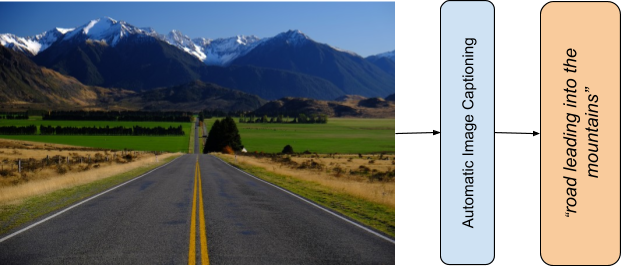
\includegraphics[width=0.6\textwidth]{figs/ch1/image-captioning.png}
	\caption{Image captioning can help millions with visual impairments by converting images captions to text. Image by \href{https://www.flickr.com/photos/francisvallance/}{Francis Vallance (Heritage Warrior)}, used under \href{https://creativecommons.org/licenses/by/2.0/}{CC BY 2.0 license}.}
	\label{fig:image-captioning}
\end{figure}

In addition to the aforementioned application of image captioning to help the visually impaired, there are many other use cases in which automatic image descriptions may help. In general, any domain in which images need to be interpreted by humans, but human availability is scarce or it is a tedious task, may benefit from an automated approach to image description.

A specific use case is the analysis and extraction of information from videos. Some video monitoring tasks are very boring and tedious. An automated mechanism to describe scenes in video footage will be of great utility for creating summaries or monitoring specific situations and events. \footnote{As an interesting example, Shell is conducting a pilot study using deep-learning to automatically monitor video footage in order to identify safety hazards and generate alerts (\href{https://customers.microsoft.com/en-us/story/shell-mining-oil-gas-azure-databricks}{link})}.

Another potential utility of automatic image description lies in the task of searching images. Having automatically generated captions for images that originally hasn't been described, would help finding images based on a complex description rather that a simple collection of tags.

\section{Goals}

This project aims at advancing in the task of automatically generating image descriptions. That is the ultimate goal of the project. However, in order to achieve such an abstract goal, we decompose it into various subgoals, as follows:

\begin{enumerate}
\item Get a solid understanding of the problem at hand and review the state-of-art solutions to it
\item Get practical knowledge on the technologies required to solve this problem
\item Develop a model using a benchmark dataset like the Flickr30K
\item Scale the model to a larger benchmark dataset such as the COCO\cite{Lin2014} dataset or the more recent Conceptual Captions Dataset by Google \cite{Sharma2018}  (see Figure \ref{fig:conceptual-captions}).
\item Evaluate the model, ideally partaking in some challenge or competition, like the ones using the COCO dataset or the Conceptual Captions dataset.
\end{enumerate}

\begin{figure}[h]
	\centering
	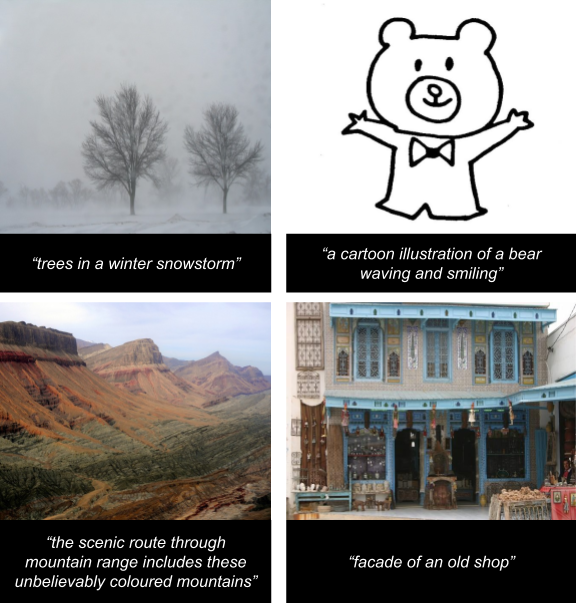
\includegraphics[width=0.6\textwidth]{figs/ch1/conceptual-captions-example.png}
	\caption{Illustration of images and captions in the Conceptual Captions dataset.Clockwise from top left, images by Jonny Hunter, SigNote Cloud, Tony Hisgett, ResoluteSupportMedia. All images used under \href{https://creativecommons.org/licenses/by/2.0/}{CC BY 2.0 license}.}
	\label{fig:conceptual-captions}
\end{figure}

\section{Methodology}

This project is mainly an academical, research-oriented project, so it would follow a process model which is common for these kind of projects, for instance, it will include a comparatively long review of the state of the art, as well as a public defense at the end. However, this project will also include the development of a software artifact to solve a data-analytic problem, therefore we should benefit from using a data-analytic model as the well known and widely adopted \textbf{CRISP-DM}. CRISP-DM, which stands for \textit{Cross-Industry Standard Process for Data Mining}, is an open standard process model and an industry-proven methodology to guide data mining projects.

As a methodology, it includes descriptions of the typical phases of a project, the tasks involved with each phase, and an explanation of the relationships between these tasks.

As a process model, CRISP-DM provides an overview of the data mining life cycle.

Figure \ref{fig:crisp-dm} depicts the relationships between the different phases of the CRISP-DM model. The sequence of the phases is not strict and moving back and forth between different phases is often required. The arrows in the process diagram indicate the most important and frequent dependencies between phases. The outer circle in the diagram symbolizes the cyclic nature of data mining itself. A data mining process continues after a solution has been deployed. The lessons learned during the process can trigger new, often more focused business questions, and subsequent data mining processes will benefit from the experiences of previous ones.

\begin{figure}[hpt]
	\centering
	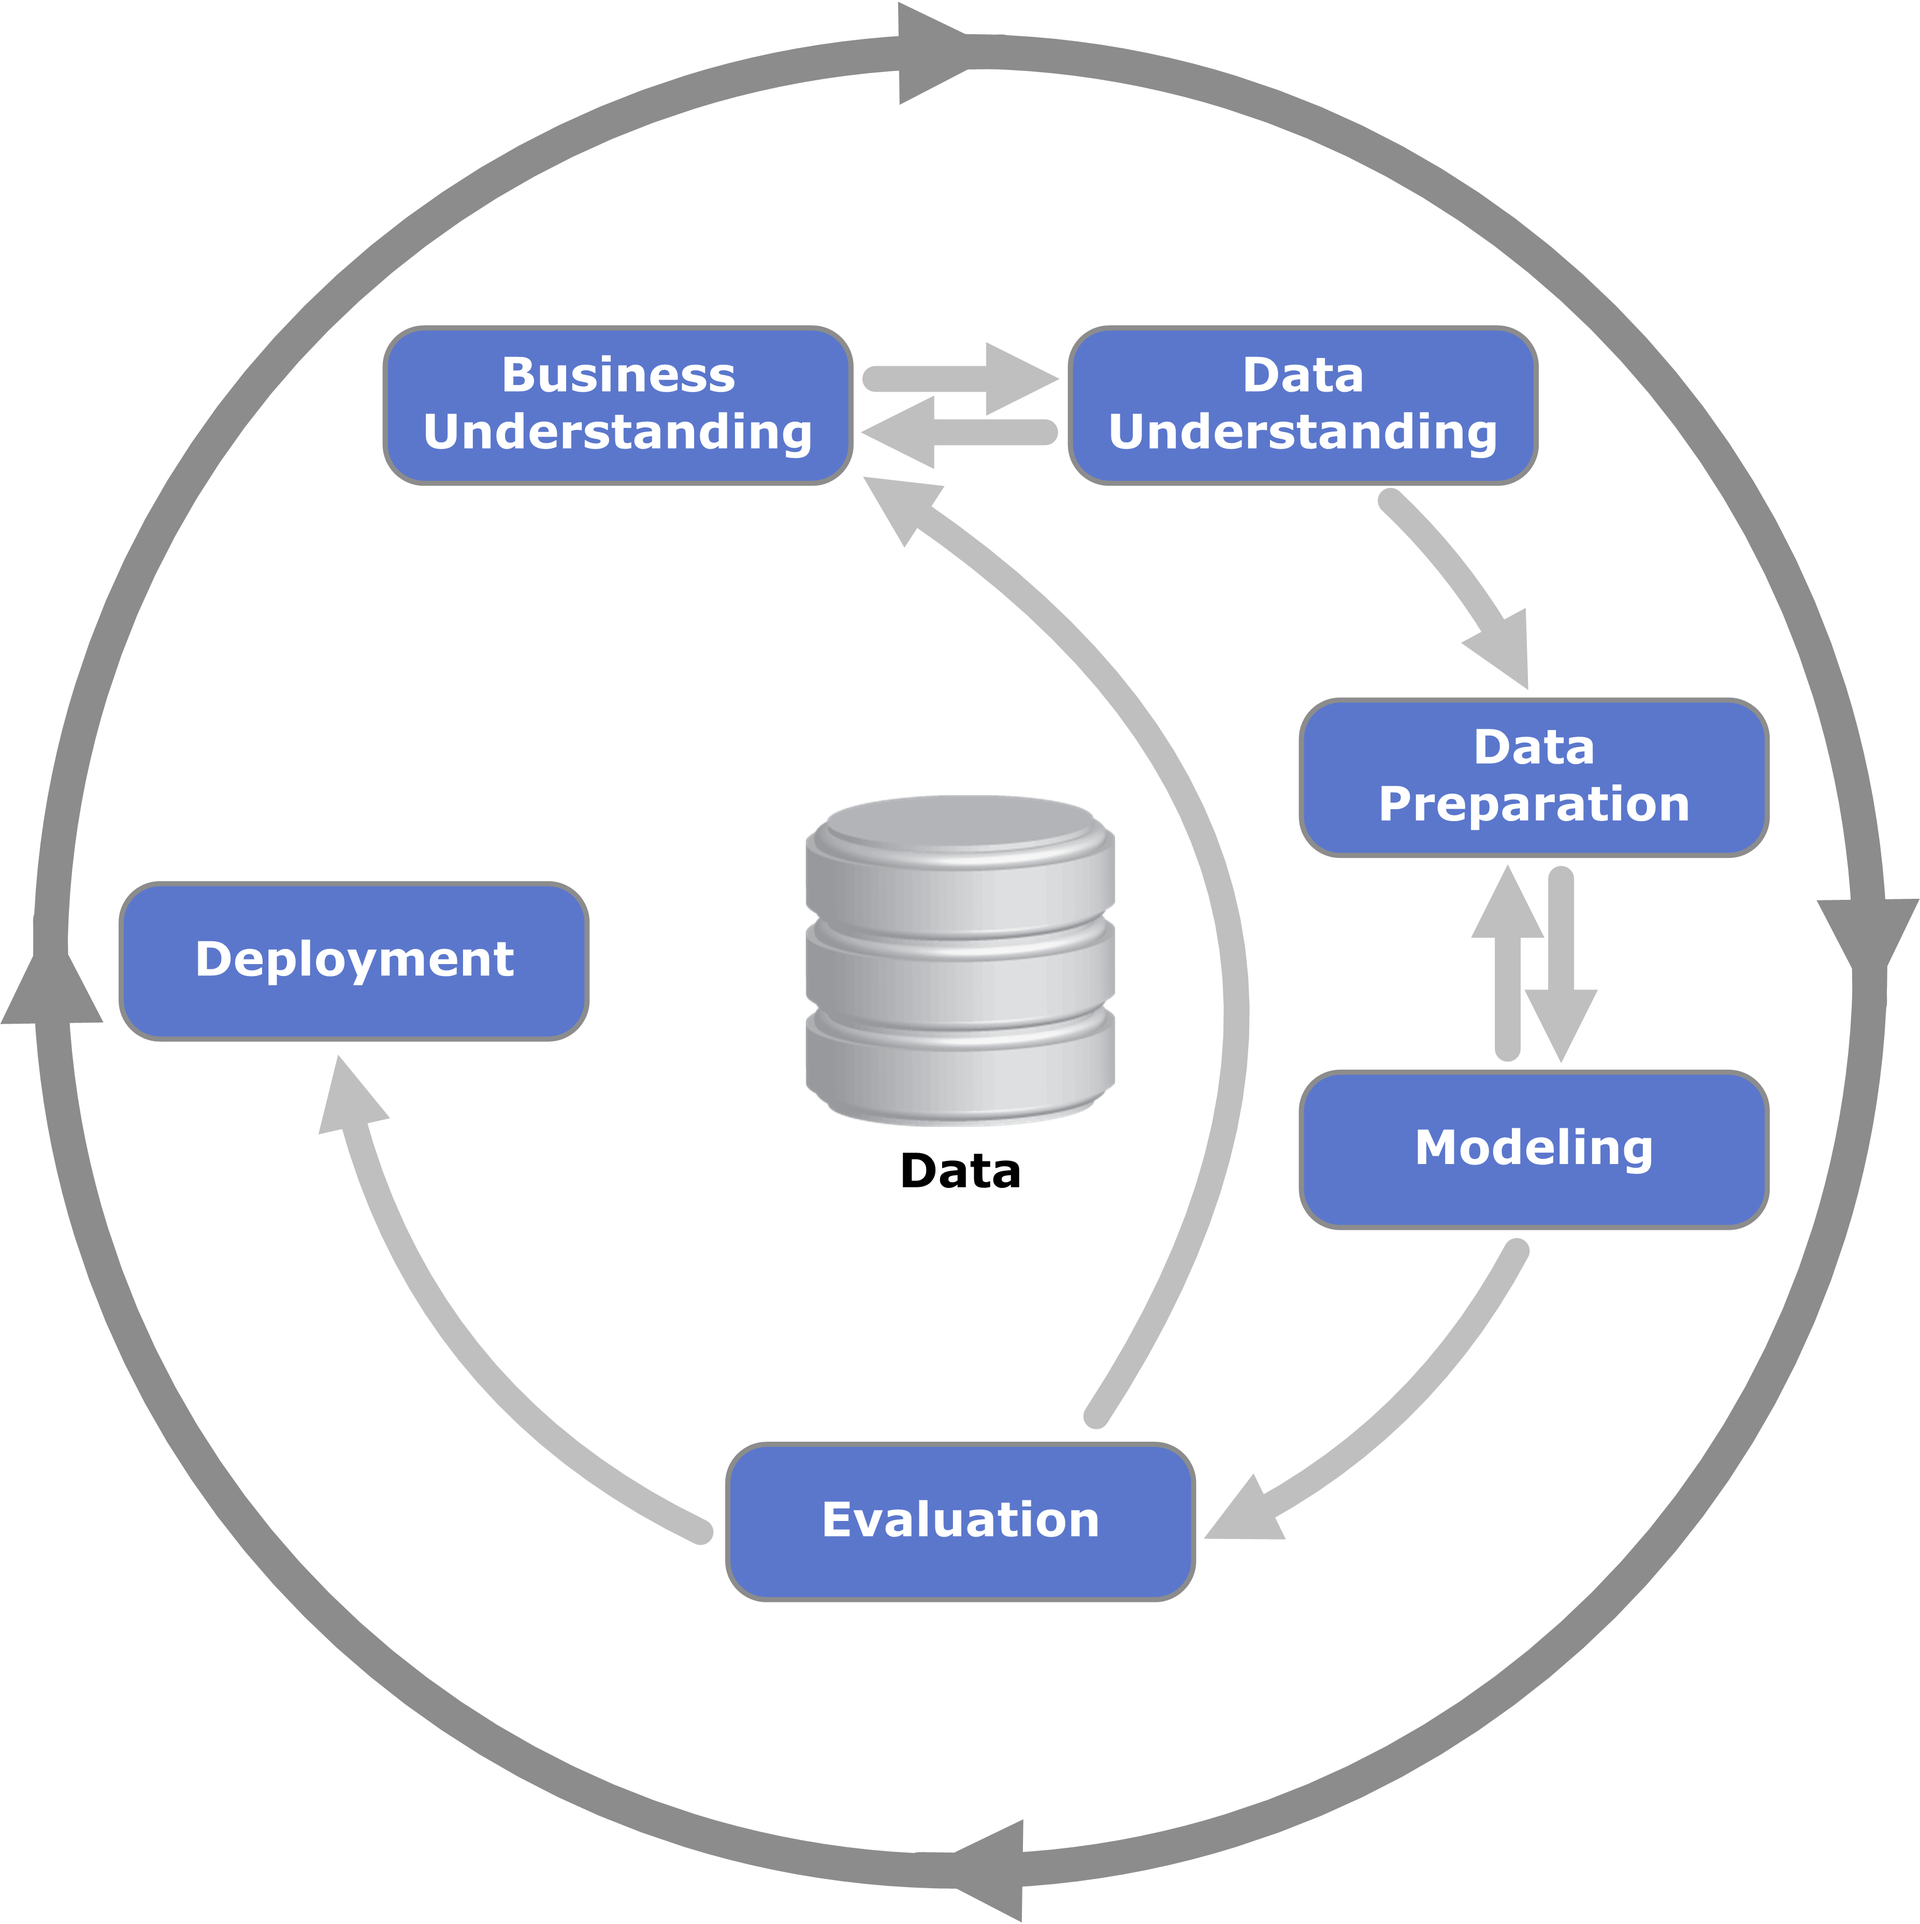
\includegraphics[width=0.6\textwidth]{figs/ch1/crisp-dm.png}
	\caption{Process diagram showing the relationship between the different phases of CRISP-DM. Image by Kenneth Jensen, used under \href{https://creativecommons.org/licenses/by/2.0/}{CC BY-SA 3.0 license..}}
	\label{fig:crisp-dm}
\end{figure}

The process model consists of six major phases:

\begin{itemize}
\item \textbf{Business Understanding}: Includes an in-depth analysis of the business objectives and needs. The situation is assessed and the goals of the project are defined. This should follow the setting up of a plan to proceed.
\item \textbf{Data Understanding}: Conduct initial or exploratory data analysis to become familiar with data and identify potential problems. Examine properties of data and verify its quality by answering questions concerning the completeness and accuracy of the data.
\item \textbf{Data Preparation}: After the data sources are completely identified, proper selection, cleansing, constructing and formatting should be done before modelling. 
\item \textbf{Modeling}: Modeling is usually conducted in multiple iterations, which involve running  several models using the default parameters and then fine-tune the parameters or revert to the data preparation phase for additional preparation. Usually, there are different ways to look at a given problem, so it is convenient to build multiple models,
\item \textbf{Evaluation}: The results of models are evaluated in the backdrop of business intentions. New objectives may sprout up owing to the new patterns discovered. This is, in fact, an iterative process, and the decision whether to consider them or not has to be made in this step before moving on to the final phase
\item \textbf{Publication}. The final information gathered has to be presented in a usable manner to the stakeholders.  This has to be done as per their expectations and business requirements.
\end{itemize}


\section{Planning}

Main tasks and milestones

\begin{table}[hbt]
\begin{tabular}{|l|l|l|}
\hline
Phase   & End  & Description   \\ \hline
1 & 3/3/2019 & Definition and planning  \\ \hline
2 & 24/3/2019 & State of the Art \\ \hline
3 & 19/5/2019 & Development \\ \hline
4 & 9/6/2019 & Complete this report \\ \hline
5 & 16/6/2019 & Presentation
\end{tabular}
\end{table}

Phase 2: this phase will encompass the following tasks:
\begin{itemize}
\item Reviewing relevant bibliography
\item Studying the problem domain (business understanding), and becoming familiar with the data. At this stage we would also start preparing the data for the modeling stage
\end{itemize}

Phase 3: this will be the longest phase, and it will include the following tasks  
\begin{itemize}
\item Preparing the data. Although data preparation could be started during phase 2, depending on the chosen models it could be necessary to conduct some additional data preparation operations
\item Generating one or various models. We plan at creating at least two models, one that would replicate existing work, and another one to explore new ideas and try to beat the baseline model.
\item Evaluating the models, and very specifically, compare our model against the replicated model.
\item Publication: We consider two courses of action: a) participating in the Conceptual Captions Challenge by Google, and b) delivering some product to the final user, although it would be a very basic prototype given the little time available.
\end{itemize}

In phase 4 we will complete this report. We would probably overlap this task with some of the tasks in phase 3 that will required more time, like the evaluation of the models and the participation in challenges.

In phase 5 we will present the results achieved for its evaluation. These results will include the code, the documentation and a public defense of the project in front of an academic board


\chapter{State of the Art}
\label{ch:state_of_the_art}

Recently there have been an upsurge of interest in problems that require a combination of linguistic and visual information. Besides, the rise of social media in the web has made available a vast amount of multimodal information, like tagged photographs, illustrations in newspaper articles, videos with subtitles, and multimodal feeds on social media. To tackle combined language and vision tasks and to exploit the large amounts of multimodal information, the CV and NLP communities have been increasingly cooperating, for example by organizing combined workshops and conferences. One such area of research in the intersection of both worlds is automatic image description.

\textbf{Automatic image description} can be defined as the task of automatically generating a description of an image using natural language. It is a very challenging problem that combines two different problems into a single task: on the one hand, there is the problem of understanding an image, which belongs to the \textbf{Computer Vision (CV)} field, one the other hand, there is also the problem of generating a meaningful and grammatically-correct description of the image, which belongs to the \textbf{Natural-Language Processing (NLP)} field, and to be more precise, it belongs to the class of \textbf{Natural-Language Generation (NLG)} problems.

Both CV and NLP are challenging fields themselves. While both fields share common techniques rooted in artificial intelligence and machine learning, they have historically developed separately, with little interaction between their scientific communities.  Recent years have seen considerable advances in both fields, to a great extent thanks to the application of deep-learning techniques and the recent advances in this area. This chapter presents a brief survey of the recent literature on this topic, including some antecedents, but focusing primarily on the recent advances coming from the application of \textbf{Deep Learning} technology, since this is our main interest.

The chapter is organized in various sections. First section is devoted to further delimiting the task at hand as well as introducing classification system for the different approaches to the problem. Subsequent sections review relevant publications organized according to the provided classification scheme. Finally, there is a section describing the datasets used by the community to benchmark their models and a short discussion on the evaluation metrics for this kind of tasks.

\section{Task definition and classification of methods}\label{sec:task-definition}

We have already defined the task of automatic image description as the task of automatically generating a description of an image using natural language generation. However, this definition is too generic to precisely characterize the task we are interested in. For example, when presented with certain image, an algorithm may generate a list of labels describing different elements of the image, or it may describe technical features of the image, such as the dimensions, the predominant colors, brightness, etc. Therefore, we need a more concrete definition of the task.

When talking about \textbf{automatic image description}, we refer to descriptions that meet three properties:
\begin{itemize}
\item Descriptions that are relevant, that is, that talk about the elements of the image.
\item Descriptions that are expressed as natural language, using grammatically correct sentences
\item Descriptions that are comprehensive but concise at the same time, that is, the description should aim at summing up the important elements of the image, not just describing it.
\end{itemize}

From the CV point of view, this task requires \textbf{full image understanding}: the description should demonstrate or pretend a good understanding of the scene, far beyond simply recognizing the objects in the image. This means that the description is able to capture relations between the objects in the scene, and the actions happening there.

From the NLP point of view, this task requires \textbf{sophisticated natural language generation} (NLG), which involves: selecting which aspects to talk about (content selection), sorting and organizing the content to be verbalized (text planning), and finally generating a semantically and syntactically correct sentence (Surface realization).

Intuitively, descriptions should be easy to understand by a person, and that person should be able to grasp the essence of the image, to create a mental model of the image without actually seeing it. The description task can become even more challenging when we take into account user-specific tailored descriptions. For instance, when describing the paintings available in a museum, a tourist may require a different description than a librarian or an art critic.

Since 2011 there have been a considerable advance in challenging CV tasks, to a great extent fostered by the application of deep learning models and the availability of large corpus of data available to researchers. More recently, a similar process seems to be occurring in the NLP field. Not surprisingly, these advances in both CV and NLP have also propelled a new wave of interest in cross-disciplinary research problems involving both areas of research, and automatic image description is a very good example. As a consequence, the CV and NLP communities have increased cooperation, for example by organizing joint workshops over the past few years. These efforts have resulted in a surge of new models, datasets and evaluation measures, which is reflected in the increase of publications, specially from 2014. 

In order of ease of review, understanding and comparison of the growing amount of research on the topic, existing surveys have proposed various schemes to classify the models being used.

One the one hand, the survey by \citet{Bernardi2017} proposes a classification system based on two dimensions and only tree categories. On the other hand, \citet{Bai2018} organize the existing research according to the kind of architecture or framework used, resulting in a more fine grained classification with 8 categories. 

After comparing both both approaches to classify the existing research, we  prefer the approach adopted by \citet{Bai2018} as we consider it more precise and descriptive,  resulting in a finer granularity; while the classification by \cite{Bernardi2017} is more abstract, resulting in a coarser granularity. A more recent survey by \citet{Hossain2019} takes the same approach found in \citep{Bai2018} with a more focused review of deep-learning based models and references to the most recent work published so far.

Below we provide a short overview of the publications covered in this survey organized into categories and sorted by publication year:

\begin{table}[ht]
\centering
\caption{Summary of published research on the automatic image description problem.}
\label{tab:overview}
\begin{tabular}[t]{p{0.3\textwidth} p{0.7\textwidth}}
    \toprule
    Approach & Representative research\\
    \midrule
    Retrieval-based & \citet{Farhadi2010, Ordonez2011, Gupta2012, Kuznetsova2012, Hodosh2013a, Kuznetsova2014, Mason2015, Hodosh2013b}\\
    Template-based &  \citet{Yang2011, Kulkarni2011, Li2011, Mitchell2012, Ushiku2015}\\
    Earlier Deep Models &  \citet{Socher2014, Karpathy2014, Ma2015, Yan2015, Lebret2015a, Yagcioglu2015}\\
    Multimodal learning & \citet{Kiros2014_VS, Mao2015_mRNN, Karpathy2015, Chen2015}\\
    Encode-Decoder framework & \citet{Kiros2014_LBL, Vinyals2015, Donahue2015, Jia2015, Wu2016, Pu2016_DGDN, Gan2017_Style, Hao2018}\\ 
    Compositional architectures & \citet{Fang2015, Tran2016, Ma2016, Oruganti2016, Wang2016_Parallel, Fu2017, Gan2017_SCN}\\
    Attention-guided & \citet{Xu2015, You2016, Yang2016_RevNet, Zhou2017, Khademi2018, Anderson2018_BUTD, Jiang2018}\\
    Describing novel objects & \citet{Mao2015_Child, Hendricks2016}\\ 
    Other deep learning methods & \citet{Pu2016_VAE, Dai2017_CGAN, Shetty2017, Ren2017, Rennie2017, Zhang2017, Anderson2018_SemiSup, Feng2018, Gu2018, Li2018_CAL, Li2018_VS-LSTM, Lindh2018}\\
    \bottomrule
\end{tabular}
\end{table}

% Skipped Wang2016_Unified, Chen2017_StrucCap, Chen2017_RLSTM, Dai2017_CL, Zhang2019, Cao2019, He2019,

\section{Early work: methods that are not based on deep learning}\label{sec:first-methods}

This section reviews the initial attempts to solve the image captioning problem. All these methods have in common that they do not use deep learning techniques. We divide them into two groups: retrieval based approaches and template-based approaches.

\subsection{Retrieval-based} \label{subsec:retrieval-based_methods}

Early work on the topic was often based in the use of retrieval-based approaches, also referred to as transfer-based approaches. These approaches usually follow a two steps process. During the first step, given a query image, a candidate set of similar images is retrieved using content-based image retrieval techniques, which are based on global image features extracted from the image. During the second step, a re-ranking of the retrieved images is computed using a variety of methods. Finally, the caption of the top image is returned, or a new caption is composed from the captions of the top-n ranked images.

\citet{Farhadi2010} use a meaning space consisting of \textit{<object, action, scene>} triplets to link images and sentences. Their model takes an input image, map it into the meaning space by solving a Markov Random Field, and use Lin's information-based similarity measure \citep{Lin1998} to determine the semantic distance between the query image and the pool of available captions. Finally, the semantically closest sentence is used as the image description.

The IM2TEXT model by \citet{Ordonez2011} uses the scene-centered descriptors of the GIST model \citep{Oliva2006, Torralba2008} to retrieve a set of similar images as a baseline, then these images are ranked using a classifier trained over a range of object detectors and scene classifiers specific to the entities mentioned in the candidate descriptions. Finally the caption of the top ranked image is returned. 

\citet{Kuznetsova2012} take on the work by \citet{Ordonez2011} with some notable twists: instead of retrieving a candidate set of images using content --visual-- features, their model start by running the detectors and scene classifiers used in the re-ranking step of the IM2TEXT model to extract and represent the semantic content of the query image. Then, instead of performing a single retrieval step to get neighbors of the query image, their model carries out a separate retrieval step for each visual entity detected in the query image. The result of this step is a collection of phrases of different type (noun and verb phrases and prepositional phrases). Finally, a new sentence is composed from a selected set of phrases using a constrain optimization approach. A refinement of the former approach is presented in \citet{Kuznetsova2014}, based on the use of tree structures to improve the sentence generation process.

\citet{Gupta2012} combine the image features of the GIST model with RGB and HSV color histograms, Gabor and Haar descriptors, and SIFT \citep{Lowe2004} descriptors for the retrieval step. Then, instead of using the visual features for the ranking step, their model relies on the textual descriptions of the retrieved images, which are segmented to obtain phrases of different type. This model takes the phrases associated to the retrieved images, rank them based on image similarity, and integrate them to get triples of the form \textit{( ((attribute1, object1), verb), (verb, prep, (attribute2, object2)), (object1, prep, object2) )}. Finally, the tree top-n triplets are used to generate an image description.

\citet{Hodosh2013b} employ a Kernel Canonical Correlation Analysis (KCCA) \citep{Bach2003} technique to project images and text items into a common space, where training images and their corresponding captions are maximally correlated. In the new common space, cosine similarities between images and sentences are calculated to rank the sentences, which are then used to select the top-n captions. This work is highly focused on the problems associated with existing benchmarks datasets and the evaluation metrics, and as a result the authors introduce a new dataset composed of 8000 images annotated with 5 captions per image, and propose a new metric based on binary judgments of image descriptions.

\citet{Mason2015} use visual similarity to retrieve a set of candidate captioned images. Second, a word probability density conditioned on the query image is computed from the retrieved captions. Finally, the candidate captions are scored using the word probability density and the one with the highest score is selected. 

An detailed analysis of the literature reviewed here reveals at least two dimensions that may further help in understanding and organizing the research: on the one hand, some approaches simply select one of the retrieved sentences as the image caption, while others compose a new caption by combining elements from several sentences; on the other hand, some approaches use visual detectors to find similar images (Content-Based Image Retrieval), while other approaches use conceptual information (Concept-Based Image Retrieval), or use a combination of visual and conceptual information for the retrieval step. \Cref{tab:retrieval-classification} sums up the various dimensions used to classify retrieval-based methods to the image captioning problem.

\begin{table}[ht]
\centering
\caption{Classification of retrieval-based image captioning.}
\begin{tabular}[t]{p{0.3\textwidth}p{0.35\textwidth}p{0.35\textwidth}}
    \toprule
    Approach & Representative research\\
    \midrule
    Information modality & Select one caption & Compose caption \\
    Visual & \citet{Farhadi2010, Mason2015} & \cite{Gupta2012} \\
    Conceptual &  \cite{Ordonez2011} & \citet{Kuznetsova2012, Kuznetsova2014} \\
    Hybrid &  \citet{Hodosh2013b} & \\
    \bottomrule
\end{tabular}
\label{tab:retrieval_classification}
\end{table}

The main disadvantage of Retrieval-Based approaches comes from its reuse of existing images. The sentences used to describe images in the past may be completely inadequate for describing a new image. Although some of the proposed models are able to compose new sentences rather than just returning one of the stored sentences, these are still based on previously used sentences, so the result may still be unsuited for describing the query image. This limitation was specially evident with the use of small datasets, therefore, perhaps the problem would be alleviated with the use of very large datasets as the ones that have appeared recently \citet{Lin2014, Sharma2018}.

\subsection{Template-based approaches}\label{subsec:template-based_methods}

Another group of early attempts to solve the automatic image captioning problem take some kind of template-based approach. Unlike retrieval based approaches, template-based approaches analyze the query image to generate concepts, and then use some kind of constraining mechanism to compose a sentence. The constrains typically adopt the form of a template, but can also be specified as grammar rules.

For example, \citet{Yang2011} use a quadruplet consisting of \textit{<Noun-Verb-Scene-Preposition>} as template for generating image descriptions. The process starts with the execution of detection algorithms to estimate objects and scenes in the image, and then apply a language model trained over the Gigaword corpus\footnote{https://catalog.ldc.upenn.edu/LDC2003T05} to compute nouns, verbs, scenes and prepositions that might appear in the caption. Finally, they apply Hidden Markov Model Inference to compute probabilities for all the elements, and use the elements with the highest probabilities to fill the template and generate a new sentence.

\citet{Kulkarni2011} employ Conditional Random Field (CRF) to determine image contents, which results in a graph with nodes corresponding to objects in the image, object attributes, and spatial relationships between objects. Unary potential functions are computed for nodes in the graph, while pairwise potential functions are obtained on a collection of existing descriptions. Afterwards, CRF inference is used to determine the image contents to be described, and finally a sentence template is applied to generate sentence using the selected content.

\citet{Li2011} use visual models to detect objects, attributes and spatial relationships, and. Then, they resort to web-scale n-gram data to compute frequency counts of possible n-gram sequences to fill a triplet defined as \textit{<(adj1, obj1), prep, (adj2, obj2)>}. Finally, dynamic programming is applied to find an optimal set of phrases that constitute the description of the query image.

\citet{Mitchell2012} apply algorithms that are able to represent an image as an <objects, actions, spatial relationships> triplet. Syntactically informed word co-occurrence statistics are computed and used by a sentence generator to filter and constrain the output of the image processor using tree structures.

The aforementioned works in this section produce new sentences based on individual words (nouns, adjectives, verbs, prepositions, etc.) that generated in a piece-wise manner from the query image, and these words are later connected according to certain grammar model. To improve on this approach, some authors have proposed the use of phrases instead of individual words. In particular, \citet{Ushiku2015} present a method named Common Subspace for Model and Similarity (CoSMoS). CoSMoS obtains a subspace in which all feature vectors associated with the same phrase are mapped as mutually close, classifiers for each phrase are learned, and training samples are shared among co-occurring phrases. Phrases estimated from a query image are connected by using multi-stack beam search to generate a description.

Template-based approaches to automatic image captioning may improve the relevance of the resulting captions when compared with retrieval based approaches, template-based captions tend to be too rigid, thus resulting in a lack of naturality when compared to human-written sentences.

\section{Deep-learning approaches}\label{sec:deep-learning_methods}

Convolutional Neural Networks (CNN) were first introduced by Yann LeCun in 1998 \citep{Lecun1998}, but it was not until more than a decade later than they started to shine. In 2012, a large, deep CNN \citep{Krizhevsky2012} was used to win, by a incredibly wide margin, the 2012 ImageNet Large-Scale Visual Recognition Challenge. From that turning point, the field has attracted attention of researchers from various fields and gained howling popularity. The success of CNN and other deep learning models was due to a great extent to its impressive results in many challenging problems, specially in the fields of Computer Vision and Natural Language Processing, where deep-learning models have became the state of the art. Not surprisingly, researchers have attempted to apply deep neural networks to solve problems in the interstice of both fields, CV and NLP, includes the problem of automatically generating image descriptions.

Recent advances in the field have been achieved with the introduction of new architectures and frameworks, accompanied by increasingly larger datasets to feed those deep neural networks. Therefore, there is a wide repertoire of methods for tackling the image captioning tasks. This section presents the contributions to the field organized according to the kind of architecture or framework utilized, with one subsection per category

\subsection{Earlier Deep Models}\label{subsec:earlier_deep-learning_models}

Encourage by the success of CNNs to solve image classification tasks, researchers began incorporating deep models into their image captioning methods, yet still influenced by the retrieval-based and template-based methods. Image captioning was formulated as a multi-modality embedding \citet{Frome2013} and ranking problem.

\citet{Socher2014} use dependency-tree recursive neural networks (DT-RNN) to represent phrases and sentences as compositional vectors. Another deep neural network \citep{Le2013} is used to extract visual features from the images. Both types of  features are mapped into a common space by using a max-margin objective function. After training, sentence retrieval is performed based on similarities between representations of images and sentences in the common space.

\citet{Karpathy2014} introduce a twist in the previous model by working at a finer level, that is, instead of modelling full images, they work on a finer level by embedding fragments of images as well as fragments of sentences fragments into a common space.  An structured max-margin objective is used to explicitly associate these fragments across modalities. Image fragments are obtained by means of a Region CNN \citep{Girshick2014}. Sentence fragments are modelled as typed dependency tree relations \citep{DeMarneffe2006}. At last, a retrieval task is performed by computing image-sentence similarities that combine both a global term and a fragment-aligned term. Experimental evaluation showed that reasoning on both the global level of images and sentences and the finer level of their respective fragments improves performance on the image-sentence retrieval task.

\citet{Ma2015} take into consideration different levels of interaction between images and sentences in order to compute similarities. Their architecture combines two different deep neural networks to tackle the multimodal space: an image encoding CNN \citep{Simonyan2015} to encode visual data, and a matching CNN \citep{Hu2014} to learn the joint representation of images and sentences. The matching CNN composes words to different semantic fragments and learns the inter-modal relations between image and the composed fragments at different levels. 

\citet{Yagcioglu2015} propose a query expansion approach for improving transfer-based automatic image captioning. The core idea of this method is to translate the given visual query into a distributional semantics based form, which is generated by the average of the sentence vectors extracted from the captions of images visually similar to the input image. It is a data-driven approach, that extracts image features using the Caffe architecture \citep{Jia2014}, a Region-CNN pipeline trained on the ImageNet dataset. The original query is expanded as the average of the distributed representations of the captions associated with the retrieved descriptions \citep{Mikolov2013}, weighted by their similarity . Finally, they transfer the closest caption as the description of the input image.

\citet{Devlin2015} also utilizes CNN activations as the global image descriptor, and perform k-NN retrieve images in the training set that are similar to the query image. Then their model selects a description from the candidate descriptions associated with the retrieved, just like the approaches by \citet{Mason2015} and \citet{Yagcioglu2015}. Their approach differs in terms of how they represent the similarity between description and how they select the best candidate over the whole set. Specifically, they propose to compute the description similarity based on the \textit{n-gram} overlap \textit{F-score} between the descriptions. The model returns the description with the highest mean n-gram overlap with the other candidate descriptions, that is the one associated to the k-NN centroid.

\subsection{Multimodal learning}\label{subsec:multimodal-learning}

Retrieval-based and template-based methods to image captioning impose limitations on the capacity to describe images in the form of templates, structured prediction, and/or syntactic trees. Thanks to the advances in neural networks, new approaches emerged that were able to surpass those limitations. These methods can yield more expressive and flexible sentences with richer structures.  Multimodal neural language models constitute one way of approaching the problem from a learning perspective. In general, these models are bidirectional, that is, they are able to generate new captions for an image, but they can also be applied in retrieval tasks for both images and sentences.

\begin{figure}[hpt]
	\centering
	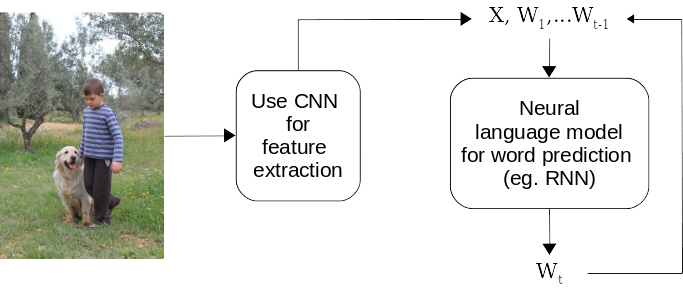
\includegraphics[scale=0.5]{ch2/multimodal.png}
	\caption{Structure of multimodal neural learning models for image captioning}
	\label{fig:multimodal}
\end{figure}

General structure of multimodal neural-based learning is shown in \cref{fig:multimodal}. First, image features are extracted using a feature extractor, typically a CNN. Then, the extracted features are forwarded to a neural-based model, which maps the image features into a common space with the word features. Finally, the model predicates new words based on the image feature and previously generated context words.

\citet{Kiros2014_VS} use a CNN for extracting image features using a multimodal space that jointly represents image and text. The key to achieve that is the use of Multimodal Neural Language Models (MNLM), that is, models of natural language that can be conditioned on other modalities. An image-text multimodal neural language model can be used to retrieve images given complex sentence queries, retrieve phrase descriptions given image queries, as well as generate text conditioned on images. The authors introduce two such languages that are adaptations of the Log-Bilinear Language Model proposed by \citet{Mnih2007}. In the case of image-text modelling it is possible to jointly learn word representations and image features by training the models together with a CNN like AlexNet \citep{Krizhevsky2012}.

\citet{Mao2014, Mao2015_mRNN} present a multimodal Recurrent Neural Network (m-RNN) model for generating novel image captions. It directly models the probability distribution of generating a word given previous words and an image, and uses this distribution to generate image captions. The model consists of two sub-networks: a deep RNN for sentences and a deep CNN for images. These two sub-networks interact with each other in a multimodal layer to form the whole m-RNN model. Besides generating captions, the m-RNN model can be applied for retrieving images or sentences. This model achieved state of art results across image captioning and image and caption retrieval tasks.

\citet{Karpathy2015} propose another multimodal approach using deep neural networks to learn embedding of image and natural language data for the task of bidirectional images and sentences retrieval. However, unlike previous methods that embed full images and sentences, this method works at a finer level, by working with fragments of images and fragments of sentences. This method applies Region-CNN to break down an image into a number of objects, RNN over sentences, represented by a dependency tree relations (DTR) \citep{DeMarneffe2006}, and a structured objective that aligns the two modalities through a multimodal embedding. The resulting Multimodal RNN architecture learns to generate novel descriptions of image regions. This model outperformed retrieval baselines on full images as well as images annotated with region-level sentences, which were derived from the MSCOCO dataset.
 
\citet{Chen2015} also explore the bi-directional mapping between images and their textual descriptions. This approach uses a RNN that attempts to dynamically build a visual representation of the scene as a caption is being generated or read. The representation automatically learns to remember long-term visual concepts. This model is capable of both generating novel captions given an image, and reconstructing visual features given an image description. The model was tested on several tasks, including sentence generation, sentence retrieval and image retrieval, and achieved state-of-the-art results for the task of generating novel image descriptions. The results for the image and sentence retrieval tasks were comparable to state-of-the-art methods using similar visual features.

In general, the multimodal approaches have limitations to handle a large amount of data and are inefficient to work with long term memory.

\subsection{The Encoder-Decoder framework}\label{subsec:encoder-decoder_framework}

The \textbf{encoder-decoder framework} was originally designed to translate sentences between different languages \citep{Kalchbrenner2013, Sutskever2014, Cho2014}. Inspired by its success solving translation problems, some researchers have adopted them to generate image captions with great success. The idea behind adapting this framework designed for translation tasks, was to see the image captioning tasks also as translation problem but across different modalities. 

\begin{figure}[hpt]
	\centering
	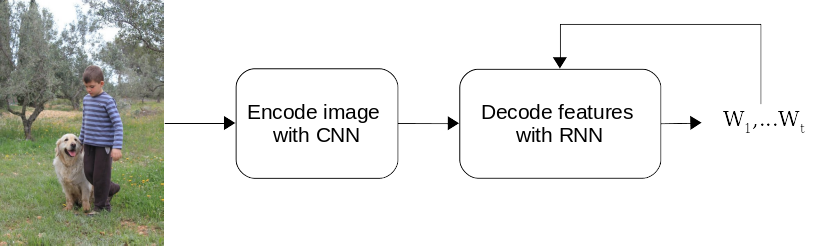
\includegraphics[scale=0.5]{ch2/encoder-decoder.png}
	\caption{Structure of image captioning methods based on the encoder-decoder framework}
	\label{fig:encoder-decoder}
\end{figure}

\citet{Kiros2014_LBL} were the first to apply the encoder–decoder framework to generate image descriptions by unifying joint image-text embedding models and multimodal neural language models. The idea is that given an image input, a sentence output can be generated word by word, like in language translation. Their model uses a Long Short-Term Memory (LSTM) \citep{Hochreiter1997} to encode textual data, and a CNN to encode visual data. Then, by optimizing a pairwise ranking loss, encoded visual data is projected into an embedding space spanned by LSTM  hidden states that encode textual data. In the embedding space, a multimodal neural language model --the so called Structure-Content Neural Language Model (SC-NLM)-- is used to decode the visual features conditioned on context word feature vectors, thus allowing for word-by-word generation of a sentence. This method achieved significant improvements in generating realistic image captions over the multimodal neural language models proposed in \citep{Kiros2014_VS}.

\citet{Vinyals2015} propose a method similar to the one by \citet{Kiros2014_VS}, which uses a CNN for image representations and an LSTM for generating image captions. This method, referred trains the LSTM based on maximum likelihood estimation. The LSTM works as follows: (1) image information is included into the initial state of the LSTM; (2)next words are generated based on the current time step and the previous hidden state; (3) this process continues until it gets the end token of the sentence. 

A problem with the former encoder-decoder methods is their susceptibility to the vanishing gradient problem, due to  image information being fed only at the beginning of the process. Consequently, the role of the initial words is also becoming weaker and weaker as the process continues. Therefore, the captions tend to degrade in relevance when generating long sentences. With the aim of mitigating this problem, \citet{Donahue2015} introduce a variation into the encoder-decoder architecture that stacks multiple LSTM atop one another. Rather than projecting the vision space into the embedding space of the hidden states at the initial stage, this model takes a copy of the static image and the previous word directly as input, that is then fed to the stack of LSTMs at each time step. This architecture, referred to as the Long-term Recurrent Convolutional Network (LRCN) model, is able to process not just static images, but also dynamic tasks involving sequences, like videos.

Still playing around with the encoder-decoder framework, some researchers propose methods to augment it by including high level semantic concepts explicitly. 

\citet{Jia2015} propose an extension of the LSTM model, which they call guided LSTM of gLSTM for short. This model adds semantic information from the image, and this information is included as extra input to each gate and cell state of the LSTM network, with the aim of guiding the model towards more relevant solutions, specially when generating long sentences. Semantic information is extracted in different ways. One way is by means of a cross-modal retrieval task that first retrieves image captions and then extracts semantic information from these captions Another way is by using a multimodal embedding space. Besides, this work explores different length normalization strategies for beam search to avoid bias towards short sentences, obtaining results that are on par with or better than the current state-of-the-art.

\citet{Wu2016} also incorporate high-level semantic concepts into the encoder–decoder framework in the form of attribute probabilities. To this end, the authors first mined a set of semantic attributes based on words commonly found in image captions. Second, they trained a multi-label classifier using one CNN per attribute, to predict the probability of attributes being present in the image. The trained CNNs are used to create a vector for each image that represents the probability of each attribute being present in it. For the caption generation, prediction vector is passed to an LSTM. For different tasks, different language models may be used, and specifically, for image captioning they adopt the region-based multi-modal language model by \citet{Vinyals2015}. The model is also capable to incorporate external semantic information and doing so further improves performance.

A circumstance that may limit the practical application of the majority of approaches discusses so far will occur when the availability of captions is limited to just a fraction of the available images. In that case, a semi-supervised learning approach would be of significant practical values. With that situation in mind, \citet{Pu2016_VAE} propose a semi-supervised learning method under the encoder–decoder framework. This method uses a Deep Generative Deconvolutional Network (DGDN) \citep{Pu2016_DGDN} as a decoder of the latent image features, and a deep CNN as an image encoder; the CNN is used to approximate a distribution for the latent DGDN features. The latent features are also linked to generative models of captions by the RNN decoder. To generate captions for new images, averaging is performed across the distribution of latent features. This framework is capable of modeling the image in the absence of associated captions, thus this is semi-supervised setting for CNN learning with images. 

\subsection{Attention-guided models}\label{sec:attention-guided_models}

Image captions should be kept short but informative. Therefore, such descriptions should mention only the most salient elements of the image, and avoid small details. Motivated by the visual attention mechanism of primates and humans \citep{Rensink2000, Spratling2004} , approaches that utilize attention to guide image description generation are proposed. By incorporating attention to the encoder–decoder framework, sentence generation will be conditioned on hidden states that are computed based on attention mechanism. The general structure of attention-guided image captioning methods is depicted in \cref{fig:attention-based} . In such methods, attention mechanism based on various kinds of cues from the input image are incorporated to make the decoding process focus on certain aspects of the input image during the caption generation process.

\begin{figure}[hpt]
	\centering
	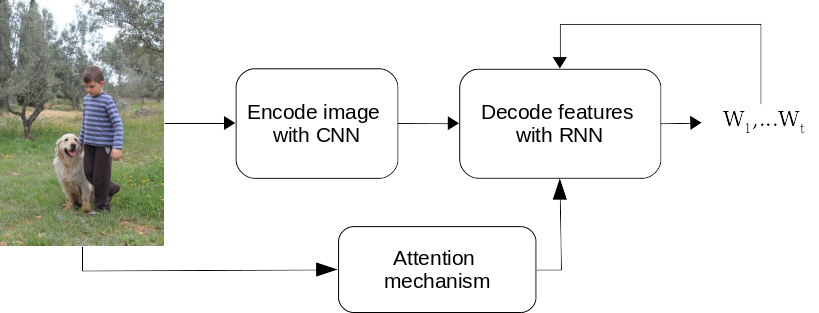
\includegraphics[scale=0.5]{ch2/attention-based.png}
	\caption{Structure of image captioning methods based on the encoder-decoder framework}
	\label{fig:attention-based}
\end{figure}

Encouraged by successes of other tasks that employ attention mechanism \citet{Mnih2014, LeiBa2015}, \citet{Xu2015} were the first to introduce an attention-mechanism to the problem of automatic image captioning. Their model, which is a variation of the encoder-decoder framework, is capable of dynamically attending salient image regions while generating the description of the image. While most approaches based on CNN image encoders use the top layer of the ConvNet for extracting image features, this method generates context vectors by using the features learned at lower layers of the ConvNet. The idea behind this approach is that the use of the top layer may result in the loss of details which may actually be useful for generating image descriptions. \citeauthor{Xu2015} have tried two different techniques for simulating attentions: stochastic hard attention and deterministic soft attention.

It is possible to classify many of the methods used in image captioning as either bottom-up or top-down. In the top-down paradigm \citep{Donahue2015, Karpathy2015, Chen2015, Mao2015_mRNN, Mao2015_Child, Vinyals2015,Xu2015} visual features are extracted first and used to select or generate a caption. In the bottom-up paradigm \citep{Farhadi2010, Kulkarni2011, Li2011, Kuznetsova2012, Elliott2013, Lebret2015a} visual concepts (e.g., regions, objects, and attributes) are extracted first and combined later to generate a caption. Top-down approaches have difficulties to deal with the fine details of an image. Bottom-up approaches, on the other hand, can operate at any image resolution and therefore are more suited for dealing with  fine details of the image. However, they have problems in formulating an end-to-end process. To take advantage of the complimentary properties of both approaches, \citet{You2016} propose a semantic attention-based method that is designed to provide a detailed, coherent description of semantically important objects. On the one hand, the visual concepts are collected using K-NN image retrieval for computing global --non-parametric-- visual concepts, and a fully convolutional network (FCN) \citep{Long2015} is trained to predict region attributes. With each attribute corresponding to one entry of the used vocabulary, words and image attributes share the same vocabulary. Under the encoder–decoder framework, the visual concepts are only forwarded to the encoder at the initial step. In the decoding stage, an LSTM is applied to decode the image features using both the global visual concepts, and the local attributes. The LSTM decoder uses two functions to generate words: an output attention function that modulates attribute attention based on the hidden state of the LSTM, and an input feedback mechanism that modulates attribute attention based on the previous word. Compared with the method introduced by \citet{Xu2015}, which works on fixed and predefined spatial location, this semantic attention-based method can work on any resolution and any location of the image.

Arguing that attention-enriched encoder–decoder models lack global modelling abilities due to their sequential information processing, \citet{Yang2016_RevNet} propose a new model called review network, which results of augmenting the encoder–decoder framework with a review module. The review network is generic and can enhance any existing encoder-decoder model.
This model performs a number of review steps with attention mechanism on the encoder hidden states, and outputs a thought vector after each review step. These thought vectors are introduced to capture the global properties of the image in a compact vector representation that is used as the input of the attention mechanism in the decoder. For example, the first review step can review what are the objects in the image?, then it can review the relative positions of the objects, and another review can extract the information of the overall context of the image. Another role for the thought vectors is as a focus for multitask learning.

\citet{Pedersoli2017} propose an area based attention mechanism for image captioning. Previous attention based methods map image regions only to the hidden state of the RNN language model. This approach, however, allows a direct association between caption words and image regions by modeling the dependencies between between image regions, caption words, and the hidden states. This associates makes the model capable of predicting the next word as well as corresponding image regions in each time-step. Another contribution of this work is the introduction of spatial transformation networks that allow for image-specific attention areas (while previous attention mechanisms used CNN activation grids, object proposals), and can be trained jointly with the rest of the network. This combination of techniques together yield state-of-the-art results on the MSCOCO dataset.

\citet{Lu2017} proposed another attention-based mechanism for image captioning using a visual sentinel. Other attention-based methods focus on the image in every time step of the recurrent neural network. However, in practice there are some words that do not need visual information (e.g. some prepositions and articles), thus applying attention to the image in these steps may be misleading and diminish the overall effectiveness of the caption generation process. To deal with this drawback, \citeauthor{Lu2017} introduce an adaptive mechanism to dynamically determine when to look at the image, and when to relay just on the language model to generate the next word. The proposed model combines a new spatial model that is able to determine where to look and a sentinel gate, which determines when to look at the image. The adaptive attention mechanism is introduced as an extension of the decoder LSTM that generates "visual sentinel" vectors (instead of just a hidden state) fallback option for the decoder. The "sentinel gate" is responsible of deciding whether to look at the image and how much information to get from it, or on the contrary, whether to relay on the visual sentinel for the caption generation process.

As we have seen, various attention mechanisms have successfully been added to deep models for improving the generation of image captions. These deep models learn dynamic weightings of the input vectors, which allow for more flexibility and expressive power than other models. Attention maps between the language space and the and language space are supposed to contain relevant information that could be useful in understanding and improving deep learning models in problems involving image and natural language, such as the image captioning problem. 

With the aim of advancing in the understanding and utility of attention mechanisms in image captioning, \citet{Liu2017_SAM} propose a quantitative method to evaluate the correctness of attention maps, which is defined as the consistency between attention maps and the corresponding regions that the words/phrases describe in the image. More specifically, \citeauthor{Liu2017_SAM} use the alignment annotations between image regions and noun phrase caption entities provided in the Flickr30k Entities dataset \citep{Plummer2015} as  ground truth maps. Using that metric, the attention-based model by \citet{Xu2015} performs better than the uniform attention baseline, but still has room for improvement in terms of attention consistency with human annotations. To improve the quality of attention maps, the authors propose the use of supervised attention, with two types of supervision: strong supervision with alignment annotation, and weak supervision with semantic labelling. In experiments, the method shows that supervised attention model performs better in mapping attention as well as image captioning tasks.

\citet{Chen2017_SCA} argue that existing visual attention based solely on spatial features have some drawbacks. To begin with, these methods compute weighted pooling only on attentive feature maps, which results in a gradual lose of spatial information. Moreover, these methods use the spatial information from the last convolution layer of the CNN, whose receptive fields correspond to very large regions, with very narrow gaps between regions; therefore, they do not get significant spatial attentions for an image. To deal with these limitations, \citeauthor{Chen2017_SCA} propose a method that combines both an spatial attention mechanism with a channel-wise attention mechanism. The new method, named SCA-CNN, extracts features not just from spatial locations, but also from different channels and multiple layers of the CNN. In addition, each filter of a convolutional layer acts as semantic detector \citep{Zeiler2014} while other methods use external sources for obtaining semantic information. In the task of image captioning, SCA-CNN dynamically modulates the sentence generation context in multi-layer feature maps, encoding where (i.e., attentive spatial locations at multiple layers) and what (i.e., attentive channels) the visual attention is. This methods outperformed visual attention-based image captioning methods across the Flickr30K and MSCOCO datasets.

To bridge the gap between humans and machines in image understanding and describing, \citet{Tavakoliy2017} study the agreement between bottom-up saliency-based visual attention and object referrals in scene description constructs. As a result of the study, \citeauthor{Tavakoliy2017} propose a saliency-boosted image captioning model that investigates possible benefits from low-level cues in language models. There are two main conclusions of the study: first, that humans mention more salient objects earlier than less salient ones in their descriptions; and second, the better a captioning model performs, the better attention agreement it has with human-generated descriptions. The authors found that the proposed saliency-boosted model does not improve significantly when the task is well learnt, but they observed a better generalization of their model when applied upon unseen data.

Visual attention plays an important role to understand images and demonstrates its effectiveness in generating natural language descriptions of images. On the other hand, recent studies show that language associated with an image can steer visual attention in the scene during our cognitive process. Inspired by this, \citet{Mun2017} introduce a text-guided attention model which learns to drive visual attention using associated captions. This model introduces an exemplar- based learning approach that retrieves from training data associated captions with each image, and use them to learn attention on visual features. This attention model enables to describe a detailed state of scenes by distinguishing small or confusable objects effectively. 

The are two main approaches to attention-based mechanisms: either use the low-level visual features to localize objects \citep{Xu2015, Lu2017}, or utilize the high-level semantic features to describe objects’ attributes \citep{Wang2017, Wu2016}, whilst the inner connections of these two types of features are not utilized. Inspired by the visual
processing of our cognitive system, \citet{Li2018_VS-LSTM} propose a model that combines low-level visual features and high-level semantic features  (attributes). The former are extracted by a Region Proposal Network (RPN), the latter are obtained by a CNN. The caption generation module is an LSTM with visual and semantic cells. The visual cell LSTM utilizes the visual features to localize the objects in the image, whilst the semantic cell LSTM further integrates the localized objects with their attributes to generate corresponding words. In addition, this method also uses Reinforcement Learning (the REINFORCE algorithm \citep{Sutton1999}) to explore proper vocabularies in the training process. The RL operates by introducing state perturbations to the LSTM units.

Top-down attention-mechanisms for building visual attention maps typically focus on some selective regions obtained from the output of one or two layers of a CNN. The input regions are of the same size and have the same shape of receptive field. \citet{Anderson2018_BUTD} argue that this approach has little consideration for the content  of the image and propose a new method inspired by the human visual system. Recent studies on human attention \citep{Buschman2007} indicate that human attention can be focused volitionally by top-down signals determined by the task at hand (e.g., looking for something), and automatically by bottom-up signals associated with unexpected, novel or salient stimuli. Inspired by this findings, \citeauthor{Anderson2018_BUTD} introduce a top-down mechanism based on Faster R-CNN \citet{Ren2015}. This mechanism proposes image regions, each with an associated feature vector, while a top-down mechanism determines feature weightings. Therefore, this method can attend both object level regions as well as other salient image regions. 

\citet{Hao2018} propose a another model based on the popular encoder-decoder architecture, but it uses the recently proposed densely convolutional neural network (DenseNet) to encode the feature maps. Meanwhile, the decoder uses an LSTM to parse the feature maps and converse them into textual descriptions. This model predicts the next word in the description by taking the effective combination of feature maps with word embedding of current input word by a visual attention switch.

\citet{Khademi2018} present a context-aware attention-based methods that employs a Bidirectional Grid LSTM (BiGrLSTM), which takes visual features of an image as input and learns complex spatial patterns based on two-dimensional context, by selecting or ignoring its input. In addition, this method leverages a set of local region-grounded texts obtained by transfer learning. The region-grounded texts often describe the properties of the objects and their relationships in an image. To generate a global caption for the image, this method integrates the spatial features from the Grid LSTM with the local region-grounded texts, using a two-layer Bidirectional Grid LSTM. The first layer models the global scene context such as object presence. The second layer utilizes a dynamic spatial attention mechanism to generate the global caption word-by-word, while considering the caption context around a word in both directions. Unlike recent models that use a soft attention mechanism, this attention mechanism considers the spatial context of the image regions.

\citet{Jiang2018} propose an extension of the encoder-decoder framework by adding a component called guiding network. The guiding network models the attribute properties of input images, and its output is leveraged to compose the input of the decoder at each time step. The guiding network can be plugged into the current encoder-decoder framework and trained in an end-to-end manner. Hence, the guiding vector can be adaptively learned according to the signal from the decoder, making itself to embed information from both image and language. Additionally, discriminative supervision can be employed to further improve the quality of guidance.

\subsection{Compositional architectures}\label{subsec:compositional_architectures}

Most of the neural methods for image captioning described in the previous sections are end-to-end systems made of tightly coupled modules whose parameters are trained jointly. An alternative architectonic approach to build such systems is based on the notion of compositional architectures, which consist of independent, loosely coupled components connected through a pipeline, where each component provides data to the next component until a final result is obtained. The idea behind this architecture is to make modular systems where it is easier to reuse existing components and replace components with little effort.

General structure of compositional image captioning methods is depicted in \cref{fig:compositional}. Usually, there are three components: 
\begin{enumerate}
\item A visual model that obtains visual features from the query image.
\item A natural language model that generates captions for the extracted features
\item A ranking module that re-ranks generated captions using a multimodal similarity model.
\end{enumerate}

\begin{figure}[hpt]
	\centering
	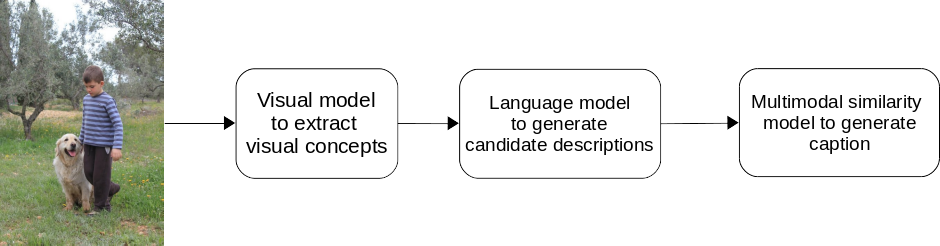
\includegraphics[scale=0.5]{ch2/compositional.png}
	\caption{Structure of image captioning methods based on the encoder-decoder framework}
	\label{fig:compositional}
\end{figure}

\citet{Fang2015} describe a system that consists of three models: visual detectors, language models and multimodal similarity models. The training process consists of two steps: First, a vocabulary of words that are most common in the training captions. Second, a visual detector is trained for each word in the vocabulary using multiple instance learning  \citep{Viola2005}. Once trained, the system can be used to generate image captions: A CNN \citep{Krizhevsky2012} is used to obtain visual features expressed as words learned vocabulary, then a maximum entropy language model \citep{Berger1996} is applied to generate candidate captions conditioned on those features. During this process, left-to-right beam search \citep{Ratnaparkhi2000} with a stack of pre-specified length $l$, produces $l$ candidate descriptions. Finally, a deep multimodal similarity model, which maps images and text fragments into a common space for similarity measurement, is used to re-rank the candidate descriptions and select the top one.

Taking on the same architecture introduced by \citet{Fang2015}, \citet{Tran2016} present a system specialized in describing landmarks and celebrities. However, instead of a CNN for the visual feature detector, this model uses a deep residual network (ResNet) to detect a broader range of visual concepts \cite{He2016a}, a maximum entropy language model for candidate description generation, and a deep multimodal similarity model for caption ranking. 

\citet{Ma2016} propose another method using a compositional architecture. Their main contribution is the introduction of structural words; tetrads composed of <objects, attributes, activities, scenes>. The method consists of two stages: structural word generation and sentence translation. At the first stage, multi-layer optimization is applied to generate a hierarchy of concepts that will play the role of structural words. During the second stage, an LSTM is used to translate the structural words into full sentences.

Realizing the high specialization of most approaches to multi-modal learning problems, \citet{Oruganti2016} introduce a more general approach called the Fusion-based Recurrent Multi-Modal (FRMM) model. This model is made of three independent components: one component per modality, and a fusion stage. Each modality is learned in a separate stage, and then their outputs are mapped to a shared representation. Finally, the fusion generates an output based on the associations between modalities it has previously learned. This approach provides the FRMM architecture increased flexibility over previous approaches in accommodating disparate inputs. The architecture for each stage might be different depending on the modalities involved, ensuring that the overall architecture is highly adaptable. The FRMM model is designed to work with multi-modal applications in which at least one of the modalities has a temporal or sequential nature, such as image description, sentiment analysis and language translation. Furthermore, two variations of the FRMM architecture are proposed according to the lengths of the inputs in each modality: Aligned FRMM (AFRMM) when the length is the same, and Unaligned FRMMM (UFRMM) otherwise. For image description in particular, the AFRMM model achieved the best results. This models obtained better results for big datasets like MSCOCO, but not for smaller datasets like Flickr30K, probably because it needs to learn more parameters than other models. 

\citet{Wang2016_Parallel} propose a parallel version of the compositional architecture with the goal of taking advantage of the complementary properties of simple RNNs one the one hand, and LSTMs networks on the other hand. There is a visual stage using CNN, as many other approaches, as well as a language generator and a fusion step. The contribution of this work lies in the parallelization of the generation and fusion stages, which consists in dividing the hidden units of the RNN into several same-size parts, and letting them work in parallel. Then, their outputs are merged with corresponding ratios for word predication. This parallelization allows for the use of different types of hidden units to combine their strengths. Specifically, the authors have used various configurations of simple RNN and LSTM. Experimental results showed a reduction in resource consumption accompanied with a simultaneous improvement in performance, compared with the dominated models (models using just one type of hidden units, either simple RNN or LSTM).

\citet{Gan2017_SCN} introduce another compositional architecture based on the encoder-decoder framework. Their model, called Semantic Compositional Network (SCN) extracts semantic tags from the image, and the probability of each tag is used to compose the parameters in a LSTM network. The SCN extends each weight matrix of the LSTM to an ensemble of tag-dependent weight matrices. The degree to which each member of the ensemble is used to generate an image caption is tied to the image-dependent probability of the corresponding tag. The same architecture can be used to describe video clips.

\citet{Fu2017} introduce an approach that aims at exploiting the parallel structures between images and sentences. In this model, the generation of the next word is aligned with the visual perception experience, where the attention shifting among the visual regions imposes a thread of visual ordering. In addition, this method uses high-level semantic information in the form of scene-specific contexts. This method works as follows: First, selective search \citep{Uijlings2013} is applied to construct a hierarchical segmentation of the image containing image regions/patches at different scales. Second, a small number of regions are selected for further processing based on the criterion of being semantically meaningful, non-compositional and contextually rich. Next, visual features are extracted from regions using a deep CNN. The sentence generation process is guided by an attention-based multi-modal LSTM decoder. The visual attention mechanism is inspired by the model described in \citep{Xu2015}, but it is enriched with information representing the scene-specific context. This information is modeled as scene vectors obtained by Latent Dirichlet Allocation (LDA) \citep{Blei2003} and a multilayer perceptron.

\subsubsection{Other approaches}

\subsubsection{Language Convolutional Neural Networks}

Since 2014, recurrent neural networks have been applied with great success to various sequence learning tasks, including the image caption generation problem. Although traditional RNNs suffer from vanishing and exploding gradient problems and cannot adequately handle long-term temporal dependencies, this problem is mitigated by modern architectures like LSTM \cite{Hochreiter1997} and GRU\citep{Chung2014}. Not surprisingly, these network architectures have also dominated the image captioning problem. 

However, LSTM/GRUs ignore the underlying hierarchical structure of a sentence. They also require significant storage due to long-term dependencies through a memory cell. In contrast, CNNs can learn the internal hierarchical structure of the sentences and they are faster in processing than LSTMs. Therefore, recently, convolutional architectures are being increasingly used in other sequence to sequence tasks,like conditional image generation and machine translation. Inspired the success of CNN in sequence learning tasks, some authors are proposing CNN as an alternative to RNN for the language generation part of their image captioning methods. The result is a CNN+CNN alternative to the dominant CNN+RNN paradigm.

The first attempt to actually use CNN for the language model of an image captioning system was the multimodal convolutional neural network (m-CNN) proposed by \citet{Ma2015}, that we already described as an earlier deep learning model. 

More recently, \citet{Gu2017} introduce a language CNN model which is suitable for statistical language modeling tasks and shows competitive performance in image captioning. In contrast to previous models which predict next word based on one previous word and hidden state, this language CNN is fed with all the previous words and can model the long-range dependencies in history words, which are critical for image captioning. However, the method cannot model the dynamic temporal behaviour of the language model using just a language-CNN, thus it combines the language CNN with a recurrent network to model the temporal dependencies properly.

\cite{Aneja2018} propose a fully convolutional architecture (CNN+CNN) for the task of image captioning. This method uses a feed-forward network without any recurrent function. The architecture of the method has four components: (i) input embedding layer (ii) image embedding layer (iii) convolutional module, and (iv) output embedding layer. It also uses an attention mechanism to leverage spatial image features. The evaluation on the MSCOCO dataset shows comparable performance to an LSTM based method on standard metrics

\citet{Wang2018} also propose a CNN+CNN image captioning method. It is similar to the method by \citeauthor{Aneja2018}, except that it includes a hierarchical attention module to connect the vision-CNN with the language-CNN. The authors of this method also investigate the use of various hyperparameters, including the number of layers and the kernel width of the language-CNN. They show how the influence of the hyperparameters can improve the performance of the method in image captioning.

\subsubsection{Reinforcement Learning}

Most image captioning methods are trained by by maximising the likelihood of ground-truth annotated captions given the image. While simple and easy to implement, this approach does not directly maximise language quality metrics such as CIDEr. In order to improve on this kind of metrics, recently proposed methods include some form of Reinforcement Learning as a way to improve the quality of generated captions with respect to this kind of metric. However, RL faces various problems when applied to language generation problems. First, unlike images, which are represented using real numbers, text processing is based on discrete numbers, which results in non-differentiable functions, making it difficult to apply back-propagation directly. However, this problem can be overcome by using the REINFORCE family of algorithms, which introduces policy gradient with differentiable function approximation \citep{Sutton1999}.

\cite{Rennie2017} propose a new optimization approach called self-critical sequence training (SCST). SCST is a form of the popular REINFORCE algorithm that, rather than estimating a base-line to normalize the rewards and reduce variance, utilizes the output of its own test-time inference algorithm to normalize the rewards it experiences. Using this approach, estimating the reward signal (as actor-critic methods must do) and estimating normalization (as REINFORCE algorithms typically do) is avoided, while at the same time harmonizing the model with respect to its test-time inference procedure. Empirically, the authors find that directly optimizing the CIDEr metric with SCST and greedy decoding at test-time is highly effective.

The method proposed by \citet{Li2018_VS-LSTM} also includes a REINFORCE algorithm to improve their captions by optimizing the CIDEr metric. This method is described in the section devoted to attention-based methods, so it is not described here again..

\cite{Zhang2017} investigate an actor-critic reinforcement learning \citep{Barto1983} approach. The architecture of this method consists of a policy network (actor) and a value network (critic). The actor treats the job as sequential decision problem and can predict the next token of the sequence. In each state of the sequence, the network will receive its evaluation metrics score as reward. The job of the critic is to predict the reward. If it can predict the expected reward, the actor will continue to sample outputs according to its probability distribution. 

The existing image captioning approaches typically train a one-stage sentence decoder, which makes it difficult to produce fine-grained descriptions. On the other hand, multi-stage sentence decoders are hard to train due to the vanishing gradient problem. \citet{Gu2018} propose a coarse-to-fine multi-stage decoder composed of a number of stacked decoders each of which operates on the output of the previous stage, producing increasingly refined image descriptions. The vanishing gradient problem is tackled by providing a learning objective function that enforces intermediate supervisions. In particular, the model is optimized with a reinforcement learning method which utilizes the output of each intermediate decoder’s test-time inference algorithm as well as the output of its preceding decoder to normalize the rewards. This method also solves the exposure bias problem and the loss-evaluation mismatch problem.

\subsubsection{Generative Adversarial Networks}

Despite phenomenal research progresses in the past several years, sentences produced by methods based on Recurrent Neural Networks tend to be rigid and lacking in variability because they learn by maximising the likelihood of ground-truth annotated captions in the training examples. This principle encourages high resemblance to the ground-truth captions, thus missing the opportunity to generate other reasonable descriptions. Conventional evaluation metrics, e.g. BLEU and METEOR, also favor such restrictive methods.

Generative Adversarial Networks (GAN) provides a possible way to generate more diverse and distinctive captions. GANs can learn deep features from unlabeled data. They achieve this representations applying a competitive process between a pair of networks: the Generator and the Discriminator. 

\citet{Dai2017_CGAN} introduce a method based on GAN with the aim to improve the naturalness and diversity of generated captions. This method, called Conditional GAN (CGAN), jointly learns a generator to produce descriptions conditioned on images, and an evaluator to assess how well a description fits the visual content. GANs face two problems when compared with RNN. First, like Reinforcement Learning, it is difficult to apply back-propagation directly, but simmilary, this problem can be tackled by introducing policy gradient mechanism with differentiable function approximation \citep{Sutton1999}. Second, sequence generation faces vanishing gradients and error propagation training difficulties. A way to mitigate this problem is to provide early feedback to the mitigator. Following this idea, CGAN adds Monte Carlo rollouts to compute future reward values at early stages of the process \citep{Yu2017}. This method only generates one caption per image.

\cite{Shetty2017} introduce another GAN based method that is able to generate multiple captions for a single image. Instead of function approximation used by other methods to deal with the discrete data backpropagation problem, this method uses Gumbel sampler \citep{Jang2017}. During training, the generator learns the loss value provided by the discriminator instead of learning it from explicit sources. The discriminator has true data distribution and can discriminate between generator-generated samples and true data samples. This allows the network to learn diverse data distribution. Moreover, the network classifies the generated caption sets into either real or fake.

\cite{Li2018_CAL} propose a conditional GAN for generating diverse captions across images. Instead of estimating the quality of a caption solely on one image, the proposed comparative adversarial learning framework assesses the quality of captions by comparing a set of captions within the image-caption joint space. The proposed architecture, called Comparative Adversarial Learning (CAL) Network consists of a caption generator and a comparative relevance discriminator which play a min-max game and optimize the loss function. With the guides from the discriminator, the generator effectively learns to generate more specific and distinctive captions, hence increases the diversity across the corpus.

\subsubsection{Other methods}

The majority of methods described in former sections are variations of the encoder-decoder framework following the CNN+RNN schema, that is to say, the encoder uses Convolutional Neural Networks \cite{Lecun1998}, and the decoder uses Recurrent Neural Networks, such as LSTM\citep{Hochreiter1997} or GRU\citep{Chung2014}.

There is also a new wave of models that replace the RNN encoder module with some form of CNN for language modelling (CNN+CNN methods) or variants of the Generative Adversarial Training, but in general all these methods still relay on a single CNN for the encoder layer. That is, the CNN feature map of the image is taken as the source input to the decoder module.

An exception to the standard CNN+RNN approach is the model proposed by \citet{Liu2017_MAT}, called MAT, which stands for Multimodal Attentive Translator. The main idea behind MAT is to view the image captioning problem as a specific form of translation task, from a sequence of objects into a sequence of words. To that aim, instead of modelling the input image as a feature map, as most CNN-based approached do, the input image has to be represented as a sequence of detected objects. In order to model the image as a sequence, MAT introduces a sequential attention layer to selectively attend to the objects that are related to generate corresponding words. Here, the input layer expands the image representation from a single CNN at a single time step in RNN, to a sequence of objects at multiple time steps. This architecture combines CNN object detectors with LSTM for the encoding module, a second  LSTM for the decoding module, plus an attention module.

The majority of deep learning approaches to the image captioning problem take the supervised learning route, with some exceptions that use some form of semi-supervised learning\citep{Pu2016_VAE, Anderson2018_SemiSup}. However, \citet{Feng2018} propose a completely unsupervised approach to train an image captioning model. Instead of relying on manually labeled image-sentence pairs, this method merely requires an image set, a sentence corpus, and an existing visual concept detector. The sentence corpus is used to teach the captioning model how to generate plausible sentences. Meanwhile, the knowledge in the visual concept detector is distilled into the captioning model to guide the model to recognize the visual concepts in an image. Furthermore, the image and caption are projected into a common latent space so that they can reconstruct each other. Given that the existing sentence corpora are mainly designed for linguistic research, the authors have also  crawled a large-scale image description corpus of two million natural sentences to facilitate the unsupervised image captioning scenario. Experimental results show promising results without any caption annotations.

\citet{Lindh2018} also introduce a form of unsupervised learning, although their model still relies on supervised learning for the most part. These authors address the low diversity and specificity in generated sentences that limits many image captioning methods by  introducing an Image Retrieval model to improve the caption specificity of the Image Captioning model. This models uses the error signal from the Image Retrieval model to improve caption specificity, which is expected to increase diversity. Training is inspired by GAN: the discriminator is replaced by the Image Retrieval module, and the generator is replaced by the Image Captioning module. But, unlike GAN, where the generator and discriminator learn from each other, in this method the discriminator is pretrained and doesn't learn from the generator. 

\subsubsection{Describing novel objects}\label{sec:novel_objects}

The image captioning methods described so far are limited to predefined vocabularies, that is, these methods are unable to generate descriptions for novel objects, objects that are not associated to any of the concepts represented in the training data (image-sentence pairs). However, humans have the ability to recognize, learn and use novel concepts in various visual understanding tasks. In practical image description applications, it is quite possible to come across situations where there are novel objects which are not included in the vocabulary learned by the model, and would be very costly to retrain the system every time a new concept appears. In this section, we describe some attempts to deal with novelties in image captioning.

In order to learn novel visual concepts without retraining the whole system, \citet{Mao2015_Child} propose a method that uses just a few images with sentence descriptions. This method is able to hypothesize the semantic meaning of new words and add them to its dictionary for future use. In order to implement and test this method, the authors have modified their previous model \citep{Mao2015_mRNN} to make it more suitable for the novel concept learning task. On the one hand, a transposed weight sharing strategy is applied to reduce the number of parameters, which in turn makes the model less prone to overfitting the new concepts. Second, an LSTM network replaces the simple RNN to avoid the gradient explosion and vanishing problem. 

Another approach to make image captioning capable of describing novel objects is the Deep Compositional Captioner (DCC), by \citet{Hendricks2016}. The DCC achieves this goal by leveraging large object recognition datasets and external text corpora, and by transferring knowledge between semantically similar concepts. First, a lexical classifier and a language model are trained over image datasets and text corpora, respectively. Then, a multimodal caption model is trained to integrate the lexical classifier and the language model using linear combinations of affine transformations of image and language features. This model enables the transfer of semantic knowledge between the two modalities, which allows generating descriptions for novel objects and their interactions with other objects. 

% \section{Other trends: ensemble methods}

\section{Datasets and evaluation}

There is a wide range of datasets available for automatic image captioning research. The images in these datasets are linked to textual captions, and differ from each other in certain aspects such as in size, the format of the captions, or the procedure used to collect the data. This section presents a brief overview of the common approaches used to collect data, the datasets themselves, and the metrics utilized for model evaluation and benchmarking.

The datasets are summarized in \cref{tab:datasets}, and examples of images their corresponding captions are given in \cref{fig:samples}. For a wider survey of datasets in the CV and NLP fields the reader is referred to \citet{Ferraro2015}. That survey is not limited to automatic image description, and provides additional statistics and quality metrics such as perplexity, syntactic complexity, and abstract to concrete word ratios.

Some authors establish a difference between image captions and image descriptions, and in this survey we have actually used them interchangeably. However, such a distinction is relevant when presenting datasets. Image descriptions verbalize what can be seen in the image, i.e., they refer to the objects, actions, and attributes depicted, etc. Captions, on the other hand, typically provide information that cannot be seen in the image or is not evident, such as personal, cultural, or historical context. Images shared through social networks or photo-sharing websites can be accompanied by descriptions or captions, or a mixture of both types of text. The images in a newspaper or a museum will typically contain cultural or historical texts, i.e., captions not 

\subsection{Datasets}\label{sec:datasets}

This subsection briefly describes the most popular datasets used in image description tasks, sorted by year of publication.

\begin{table}[ht]
\centering
\caption{Summary of benchmark datasets.}
\begin{tabular}[t]{lrccc}
    \toprule
    Dataset &  Images & Texts & Judgements & Objects \\
    \midrule
    Pascal1K \citep{Rashtchian2010} & 1K  & 5 & No & Partial \\
    IAPTR-TC12 \citep{Escalante2010} & 20K  & 1-5  & No & Segmented \\
    VLT2K \citep{Elliott2013} & 2K  & 3  & Partial & Partial \\
    Flickr8K \citep{Rashtchian2010} & 8K & 5 & Yes & No \\
    Abstract Scenes \citep{Zitnick2013} & 10K & 6 & No & Complete \\
    Flickr30K \citep{Young2014} & 31K  & 5 & No & No \\
    MSCOCO \citep{Lin2014} & 328K & 5 & Collected & Partial \\
    Conceptual Captions \citep{Sharma2018}  & 3.3M  & 1  & No & No \\
    \bottomrule
\end{tabular}
\label{tab:datasets}
\end{table}

The \textbf{Pascal1K} sentence dataset \citet{Rashtchian2010} consists of 1000 images that were selected from the Pascal 2008 object recognition dataset\footnote{Every year, the Pattern Analysis, Statistical Modeling, and Computational Learning (PASCAL) organization hosts the Visual Object Classes Challenge. In this competition, a new dataset of images with classification and detection information is released, and computer vision researchers compete to create the best classification, detection, and segmentation systems} \citep{Everingham2010}. The dataset covers a wide variety of objects and scenery classified into 20 different categories, such as humans, animals, and vehicles. Each image is associated with five one-sentence descriptions generated by humans using the \textbf{Amazon Mechanical Turk (AMT)}\footnote{Amazon Mechanical Turk (MTurk) is a crowdsourcing marketplace that makes it easier for individuals and businesses to outsource their processes and jobs to a distributed workforce who can perform these tasks virtually. This could include anything from conducting simple data validation and research to more subjective tasks like survey participation, content moderation, and more. See https://www.mturk.com/ \nopagebreak} crowdsourcing service. For the image annotation process, the Turkers (AMT workers) were instructed to focus on the images and describe their contents without considering the context.

The \textbf{IAPR-TC12} dataset \citep{Escalante2010} conatins an image collection consisting of 20k images taken from locations around the world and comprising a varying cross-section of still natural images. They were obtained by guides of an independent travel company and undergo a selection process. The images are accompanied by written descriptions expressed in multiple languages (predominantly English and German). Each image is associated with one to five descriptions, sorted by a certain priority pattern.

The \textbf{Visual and Linguistic Treebank (VLT)}  \citep{Elliott2013} makes use of images from the Pascal 2010 action recognition dataset, augmented with three descriptions of two sentences length per image. These descriptions were collected on the AMT with specific instructions to verbalize the main action depicted in the image and the actors involved (first sentence), as well as the most important background objects (second sentence). There are object annotations available for a subset of 341 images, in the form of polygons around all objects mentioned in the descriptions. Moreover, this subset also includes 3 manually-created Visual Dependency Representations (VDR) per image. 

The \textbf{Flickr8K dataset} \citep{Rashtchian2010} comprises approximately 8k images obtained from the \textit{Flickr} photo-sharing website. The images in this dataset were collected through user queries for specific objects and actions using the AMT. The descriptions consist of 5 sentences per image collected from AMT workers using a strategy similar to that of the Pascal1K dataset. 

The \textbf{SBU Captioned Photo} dataset \citep{Ordonez2011} contains around 1M images harvested from Flickr. It was the first attempt to provide a huge dataset for image captioning tasks, but further analysis showed several issues that severely diminished its utility, like captions containing information that cannot be obtained from the image itself (eg. names of people and location), captions describing just a small detail of the image, or captions consisting being a mere commentary about the image.

The \textbf{Abstract Scenes} dataset \citep{Zitnick2013} consists of 10k clip-art images and their descriptions. The images were created through AMT, where workers were asked to place a fixed vocabulary of 80 clip-art objects into a scene of their choosing. The descriptions were then sourced for these worker-created scenes. The authors provided these descriptions in two different forms. While the first group contains a single sentence description for each image, the second group includes two alternative descriptions per image. Each of these two descriptions consist of three simple sentences with each sentence describing a different aspect of the scene. The main advantage of this dataset is it affords the opportunity to explore image description generation without the need for automatic object recognition, thus avoiding the associated noise. A more recent version of this dataset has been created as a part of the visual question-answering (VQA) dataset \citep{Antol2015}. It contains 50k different scene images with more realistic human models and with five single-sentence descriptions. 

The \textbf{Flickr30K} dataset \citep{Young2014} is an extended version of the Flickr8K dataset comprising around 31k images. The images in this dataset are mainly about humans involved in everyday activities and events. Each image is described by 5 sentences, like its minor version. Moreover, unlike the 8k version, this dataset is complemented with a \textit{denotation graph} that pairs generalized versions of the image captions with their visual denotations, i.e. the sets of images they describe.

The \textbf{MS-COCO} (Common Objects in Context) dataset \citep{Lin2014}, by Microsoft, is one the largest datasets available for research in image description tasks. It includes 328k images of complex everyday scenes containing common objects in their natural context.  These images have been annotated with 5 descriptions per image, plus bounding boxes for objects belonging to 80 object categories. This dataset has been widely used for image description, something that is facilitated by the standard evaluation server that is available online since the 2015 COCO Captions Competition \footnote{Source: https://competitions.codalab.org/competitions/3221}. 

Very recently, Google launched \textbf{Conceptual Captions} \citep{Sharma2018}, a huge dataset with an order of magnitude more images than the largest dataset to date (MS-COCO), and represents a wider variety of both images and image caption styles. However, unlike former datasets, which were annotated manually by humans, the 3.3M images of this dataset were collected programmatically, by extracting and filtering images and text annotations from billions of webpages. It consists of a wide variety of images and associated descriptions taken from original Alt-text attributes, automatically transformed to achieve a balance between cleanliness, informativeness, and learnability. The remaining image, caption pairs contain around 16,000 entity types, guaranteed to be well represented in terms of number of examples.

\begin{figure}[hpt]
	\centering
	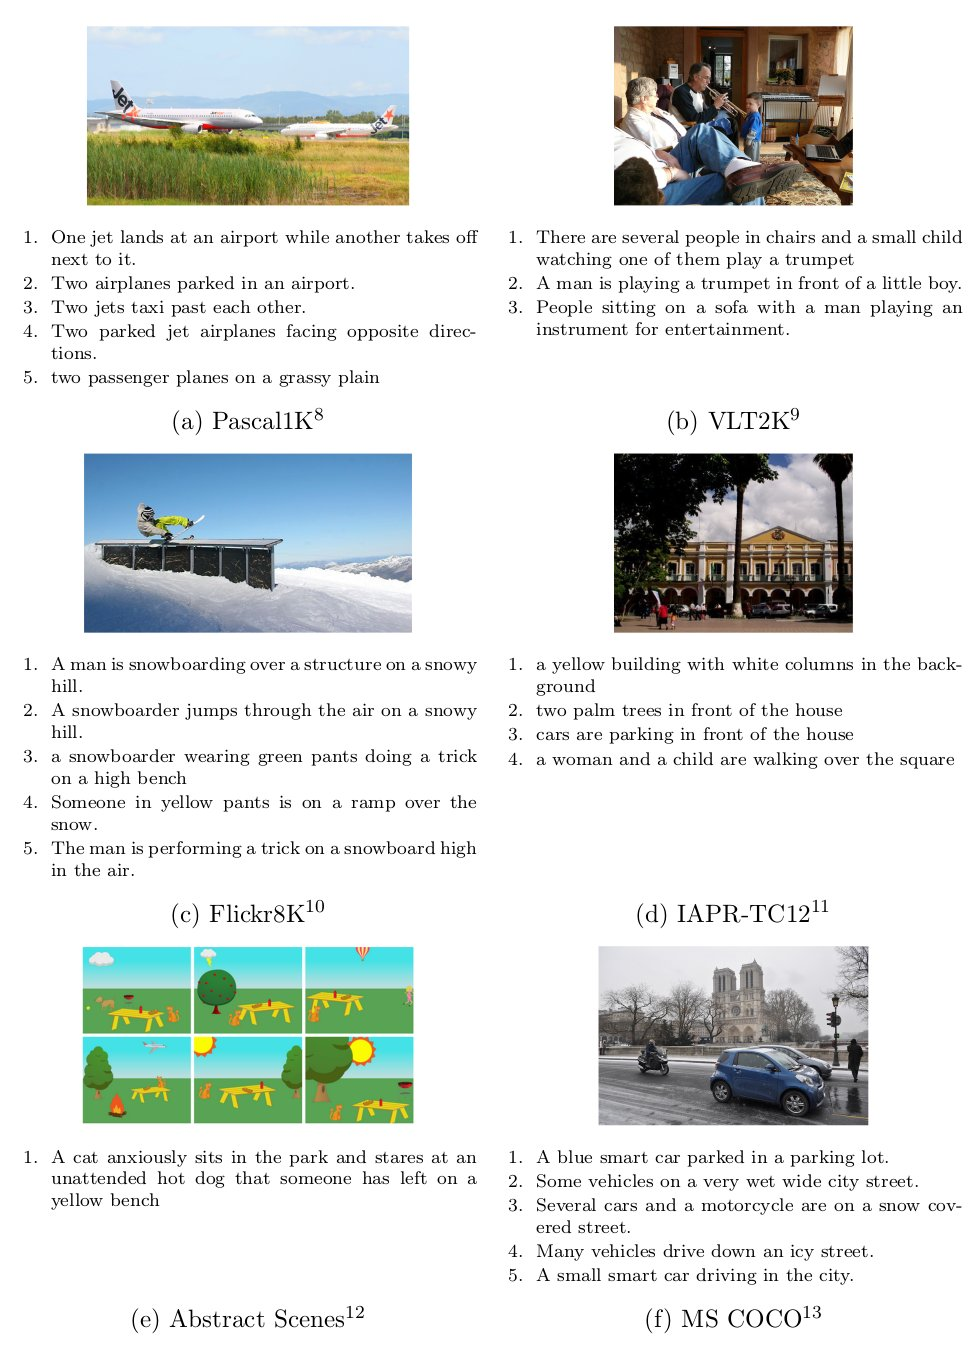
\includegraphics[scale=0.45]{images/ch2/image-caption-examples.jpg}
	\caption{Examples of images and their descriptions across various benchmark datasets}
	\label{fig:samples}
\end{figure}

\subsubsection{Other datasets}

This subsection summarizes other datasets that, in spite of being less popular that the ones already presented,  are to a certain extent relevant to the problem at hand.

\begin{itemize}
\item The Attribute Discovery dataset \citep{Berg2010} was collected using automatic dataset construction techniques that exploit the connection between text and images. This dataset consists of 4 broad shopping categories (bags, earrings, ties, and shoes). The data set was collected from \textit{like.com} and includes both images and associated textual descriptions.
\item The \textbf{MIT-Adobe FiveK} \citep{Bychkovsky2011} dataset consists of 5K images containing a diverse set of scenes, subjects, and lighting conditions. These images are mainly about people, nature, and man-made objects.
\item The \textbf{NYU-v2} dataset \citep{Silberman2012} is a more specialized dataset containing 1.5K RGBD images capturing 464 diverse indoor scenes, with detailed annotations. The particularity of this dataset is its focus on 3D segmentation. It has been augmented with five descriptions per image by \citet{Lin2015} for image description tasks.
\item The \textbf{SUN Attribute} database \citep{Patterson2014} provides around 15K  images from 707 scene categories. It was derived from the SUN categorical database using crowdsourcing to annotate images with attributes. Previously, crowdsourced human studies were preformed to find a taxonomy of 102 discriminative attributes related to varied aspects, such as materials, surface properties, lighting, affordances, and spatial layout.
\item The \textbf{FlickrStyle10k} dataset has 10K Flickr images with stylized captions. The training data consists of 7K images. The validation and test data consists of 2,000 and 1,000 images respectively. Each image contains romantic, humorous, and factual captions.
\item  The \textbf{Stock3M} dataset \citep{Wang2017} has more than 3M images uploaded by the users of a stock image website. Each image is associated with one caption that is provided by the photo uploader. The captions are much shorter than those found on the MSCOCO dataset, but are claimed to be more natural, with a larger vocabulary and image content variety.
\item The \textbf{VQA} (Visual Question Answering) dataset is intended to support a variation of the image description problem called \textit{visual question answering}: given an image and a natural language question about the image, the task is to provide an accurate natural language answer \citep{Antol2015}. To that aim, the dataset contains 50K abstract scenes using clip-art style graphics. It includes 20 paperdoll human models spanning genders, races, and ages with 8 different expressions, over 100 objects and 31 animals in various poses. The images are completed with five captions per image, as well as diverse questions and answers.
\end{itemize}

\subsection{Evaluation metrics}\label{sec:metrics}

Evaluating Natural Language Generation (NLG) systems is a fundamentally difficult task \citep{Reiter2009}, so that it has become a research problem itself. However, we will simply summarize the metrics commonly used for evaluating the quality of image descriptions generated automatically.

\subsubsection{Human judgement}

A common way to assess the quality of automatically generated texts is the subjective evaluation by human judges. Automatically produced text is usually judged in terms of syntactical correctness (grammar compliance) and semantic correctness (relevance of the content). Another dimension of interest is the fluency of the text, especially when a surface realization technique is involved in the generation process. Image descriptions generated automatically can be evaluated using the same techniques that are common in other NLG tasks, an very particularly in machine translation (MT) tasks. In this case, judges get both the image and the generated description for the evaluation task. Subjective human evaluations of machine generated image descriptions are often performed on the Amazon Mechanical Turk by means of Likert-scale questions. Some examples of these kind of questions are:

\begin{itemize}
\item The description accurately describes the image
\item The description is grammatically correct
\item The description has no incorrect information
\item The description is relevant for this image
\item The description is human like
\end{itemize}

\subsubsection{Automatic evaluation metrics}

Since human evaluation requires large amounts of non-reusable human effort, it is difficult to scale up. Furthermore, human judgement is inherently subjective, which makes it suffer from user variances. To avoid these pitfalls, automated metrics have been created with different properties. Below follows a short review of the most common metrics used for evaluating machine-generated image descriptions.

Classical \textbf{information retrieval metrics}, like the \textit{median rank} (mRank) and the \textit{precision and recall at k} (S@k, R@K) have been included quite often to evaluate the descriptions returned by image captioning methods, particularly with for methods that adopt an information retrieval approach, although they are not considered the most appropriate metric for this task.

IBM's \textbf{BLEU} (Bilingual Evaluation Understudy) \citep{Papineni2002} is a familiy of metrics conceived to substitute human judges in the evaluation of MT tasks, so besides being quick, inexpensive and language independent, it was designed to show good correlation with human judgement. This family of metrics use a weighted average of variable length phrase matches against the reference translations written by humans to measure their closeness. BLEU starts with a baseline metric from which a number of metrics are derived for different n-gram sizes: BLEU-1 compares the candidate sentence with sentences in unigram, BLEU-2 compares the candidate sentence with sentences in bigram, and so on, until BELU-4, which obtains the best correlation with human judgements While unigram scores account for the adequacy, higher n-gram scroes account for fluency. BLEU is popular because was it was the first metric popularized for MT tasks, long before the research on automatic image generation field took off. Although BLEU shows a reasonable correlation with human judgements it seems to work well only when the generated text is sort  \citep{Callison-Burch2006}, and it may even occur that an increase in BLEU score did not corresponds to an increase of quality \citep{Lin2004b}.

\textbf{ROUGE} (Recall-Oriented Understudy for Gisting Evaluation) \citep{Lin2004a} is a set of metrics introduced as an alternative to BLEU to work with larger texts, like text summaries. This metric employs the longest common subsequence between a candidate sentence and a set of reference sentences to measure their similarity at sentence-level. The longest common subsequence between two sentences only requires in-sequence word matches, and the matched words are not necessarily consecutive. Determination of the longest common subsequence is achieved by using dynamic programming. Different versions of ROUGE exist for different tasks: ROUGE-1 and ROUGE-W are appropriate for single document evaluation whereas ROUGE-2 and ROUGE-SU4 have good performance for short summaries. 

\textbf{METEOR} (Metric for Evaluation of Translation with Explicit ORdering) \citep{Banerjee2005} is another metric originally conceived to evaluate MT tasks. It is based on a generalized concept of unigram matching between the machine- produced translation and human-produced reference translations. Unigrams can be matched based on their surface forms, stemmed forms, and meanings. It first performs generalized unigram matches between a candidate sentence and a human-written reference sentence, and then computes a score based on the matching results. The score computation involves precision, recall and alignments of the matched elements, and in the case of multiple reference sentences, the best score among all the possible matches is taken as the final evaluation score. METEOR achieves better correlation at the sentence or the segment levels. There exists a \textit{Universal} version of this metric supporting many languages, like Russian and Hindi \citet{Denkowski2014}.

\textbf{CIDEr} (Consensus-based Image Description Evaluation) \citep{Vedantam2015} adopts a novel paradigm which is based on human consensus, and was designed specifically to evaluate image description tasks instead of MT tasks. This metric measures the similarity of an automatically generated sentence to the majority --consensus-- of ground-truth sentences (image descriptions) written by humans. It works by encoding the frequency of the n-grams in the candidate sentence that appear in the reference sentences using a Term Frequency Inverse Document Frequency (TF-IDF) weighting for each n-gram. While most existing datasets have only five captions per image, which the authors consider is not enough to use human consensus, therefore they also created two new datasets with 50 human-generated sentences per image: \textbf{Pascal-50S} and \textbf{Abstract-50S}, which uses the 1000 images from the Pascal1K, and 500 random images from the Abstract Scene dataset, respectively. A version of CIDEr named \textbf{CIDEr-D} is available as a part of the MSCOCO evaluation server to enable systematic evaluation and benchmarking.

\textbf{SPICE} (Semantic Propositional Image Caption Evaluation) \citep{Anderson2016} is a new evaluation metric for image descriptions based on a graph-based semantic representation of images called scene-graph \citep{Johnson2015, Schuster2015}. This graph can extract the information of different objects, attributes and their relationships from the image descriptions, and is based on the assumption than semantic propositional content is an important component of human caption evaluation. Extensive evaluations across a range of models and datasets indicate that SPICE captures human judgments over model-generated captions better than other automatic metrics. Furthermore, SPICE can answer questions such as which caption-generator best understands colors? and can caption-generators count?

\textbf{SPIDEr} \cite{Liu2017_PG} has been proposed recently to overcome some of the problems attributed to existing metrics by combining the properties of two of them: CIDEr and SPICE. This combination is achieved by means of a policy gradient (PG) method that directly optimizes a linear combination of SPICE and CIDEr (hence the name SPIDEr). SPICE score ensures semantic faithfulness of generated sentences, while CIDEr score guarantees that these descriptions are syntactically fluent.

\citep{Sharif2018} explore a learning-based approach to combine various metrics and report on their results. The idea behind this metric is the same behind SPIDEr: while some metrics tend to focus on the lexical and syntactical correctness (BLEU, ROUGE, CIDEr), other metrics tend to focus on the semantic relevance (SPICE). Therefore, combining the linguistic properties of various metrics should help achieve a better assessment of the quality of image description. Experimental results show improvements over other metrics in terms of correlation and accuracy on the Pascal-50S dataset.

\subsection{Summary of methods, datasets, metrics and benchmark results}\label{sec:summary_and_comparison}

This subsection summarises all the published research covered in this survey. We begin with an extended overview of the reviewed methods for image captioning that use deep learning techniques. We already presented an overview of methods in \cref{tab:overview}, but this time we include additional information to classify and characterize the methods. This information is described below, and it is presented in \cref{tab:classification}.

\begin{itemize}
\item The \textbf{network architecture} used to encode images. All methods use convolutional neural networks (CNN), but they differ in the specific network architecture, like VGG, Inception or ResNet, among others.
\item The kind of network used to learn the \textbf{language model}, typically some form of LSTM, but also other RNN and other models.
\item A classification of the method across multiple dimensions.
    \begin{itemize}
    \item \textbf{Visual Space (VS}) vs \textbf{Multimodal Space (MS}): Most methods model the image in the visual space, but some methods learn a combined visual and language space (see \cref{subsec:multimodal-learning})
    \item \textbf{Supervised Learning (SL}) vs \textbf{Other Deep Learning (ODL}). Although most methods use supervised learning, in some cases a form of semisupervised or unsupervised learning is employed (eg. generative adversarial networks (GAN) and reinforcement learning (RL)).
    \item \textbf{Whole Scene (WS}) vs \textbf{Dense Captioning (DC}): Most methods encode and describe images treated as a whole, but some approaches also detect regions in the image and generate descriptions for those regions.
    \item \textbf{Encode-Decoder (EDA}) vs \textbf{Compositional Architecture (CA}): many approaches adopt and encode-decoder architecture (see \cref{subsec:encoder-decoder_framework}), while only a few approaches adopt a compositional architecture (see \cref{subsec:compositional_architectures}).
    \end{itemize}
\item In addition to the above dimensions, some methods are annotated with extra descriptors to further characterize the image captioning methods:
    \begin{itemize}
    \item \textbf{Attention-Based (AB}) refers to methods that can dynamically focus on various parts of the image while the language descriptions are generated (see \cref{sec:attention-guided_models}).
    \item \textbf{Semantic Concept-Based (SCB}) methods selectively attend to a set of semantic concepts extracted from the image, so these methods apply a very specific form of attention mechanism.
    \item \textbf{Novel Object (NOB}) is used to characterize those methods that are able to describe objects that were not learned, that is, objects that were not included in the training dataset (see \cref{sec:novel_objects}).
    \item \textbf{Stylized Captions (SC)} refers to the use of styles  (eg. romantic, humorous) to generate more attractive captions. 
    \end{itemize}
\end{itemize}

Other acronyms used in this classification are:
\begin{itemize}
\item LBL: Log-Bilinear Language Model. It is a neural language model that operates on a feature vector representation of words. Word embeddings are computed using a feedforward neural network. Then, the probability of the next word is computed given the previous words (context) (see \citep{Mnih2007} for details).
\item SC-NLM: Structure-Content Neural Language Model. It is a multimodal neural language model proposed by \citep{Kiros2014_VS}
\item DTR: Dependency Tree Relations. Structure that represents all sentence relationships uniformly as typed dependency relations, that is, as triples of a relation between pairs of words (see \citep{DeMarneffe2006}).
\item MELM: Maximum Entropy Language Model. Model that predicts next word in a sentence based on the principle of maximum entropy (see \citep{Berger1996} for details).
\item HM-LSTM: Hierarchical Multimodal LSTM. Variation of the LSTM architecture proposed by \citet{Niu2017}
\item LCNN: Language CNN. Refers to the use of convolutional neural networks to represent language models \footnote{The use of CNNs for sentence modeling traces back to \citet{Collobert2008}. The ability of CNNs to create informative latent semantic representations of sentences for downstream tasks  \citet{Collobert2011,Kalchbrenner2014,Kim2014} led to a huge proliferation of CNN-based networks applied to NLP tasks.}. 
\end{itemize}

Note: In the classification presented in \cref{tab:classification}, we have omitted various methods described in the earlier works section (\cref{subsec:earlier_deep-learning_models}) that do not fit in the proposed dimensions. These methods are \citet{Socher2014, Lebret2015a, Lebret2015b, Yagcioglu2015}.

\begin{longtable}{ p{.30\textwidth} p{.20\textwidth} p{.20\textwidth} p{.30\textwidth}}
    \caption{Classification of deep-learning methods}\\
    \toprule
    Publication &  Image Encoder & Language Model & Category\endhead
    \midrule
    \citet{Karpathy2014} & AlexNet & DTR & MS,SL,WS,EDA \\
    \citet{Kiros2014_VS} & AlexNet & LBL & MS,SL,WS,EDA \\
    \citet{Kiros2014_LBL} & AlexNet, VGG & LSTM,SC-NLM & MS,SL,WS,EDA \\
    \citet{Mao2014} & AlexNet & RNN & MS,SL,WS \\
    \citet{Chen2015} & VGG & RNN & VS,SL,WS,EDA \\
    \citet{Donahue2015} & Caffe & LSTM & VS,SL,WS,EDA\\
    \citet{Devlin2015} & VGG & MELM & MS,SL,SL,WS,EDA\\
    \citet{Fang2015} & AlexNet,VGG & MELM & VS,SL,WS,EDA \\
    \citet{Jia2015} & VGG & LSTM & VS,SL,WS,CA, SCB \\
    \citet{Karpathy2015} & VGG & RNN & MS,SL,WS,EDA \\
    \citet{Ma2015} & VGG & LCNN & MS,SL,WS,EDA \\
    \citet{Mao2015_mRNN} & AlexNet,VGG & RNN & MS,SL,WS\\
    \citet{Vinyals2015} & Inception-V1 & LSTM & VS,SL,WS,EDA\\
    \citet{Xu2015} & AlexNet & LSTM & VS,SL,WS,EDA,AB\\
    \citet{Hendricks2016} & VGG & LSTM & VS,SL,WS,CA,NOB\\
    \citet{Johnson2016} & VGG & LSTM & VS,SL,DC,EDA\\
    \citet{Ma2016} & AlexNet & LSTM & VS,SL,WS,CA\\
    \citet{Mao2016} & AlexNet,VGG & LSTM & VS,SL,WS,EDA\\
    \citet{Mathews2016} & Inception-V1 & LSTM & VS,SL,WS,EDA,SC\\
    \citet{Sugano2016} & VGG & LSTM & VS,SL,WS,EDA,AB\\
    \citet{Tran2016} & ResNet & MELM & VS,SL,WS,CA\\
    \citet{Wang2016_Parallel} & VGG & LSTM & VS,SL,WS,CA\\
    \citet{Wu2016} & VGG & LSTM & VS,SL,WS,EDA,SCB\\
    \citet{Yang2016_RevNet} & VGG & LSTM & VS,SL,DC,EDA,AB\\
    \citet{You2016} & Inception-V1 & RNN & VS,SL,WS,EDA,SCB\\
    \citet{Chen2017_SCA} & VGG,ResNet & LSTM & VS,SL,EDA,AB\\
    \citet{Dai2017_CGAN} & VGG & LSTM & VS,ODL,WS,EDA\\
    \citet{Fu2017} & VGG & LSTM & VS,SL,WS,EDA,AB\\
    \citet{Gan2017_Style} & ResNet & LSTM & VS,SL,WS,EDA,SC\\
    \citet{Gan2017_SCN} & ResNet & LSTM & VS,SL,WS,CA,SCB\\
    \citet{Gu2017} & VGG & LCNN,LSTM & VS,SL,WS,EDA\\
    \citet{Liu2017_SAM} & VGG & LSTM & VS,SL,WS,EDA,AB\\
    \citet{Liu2017_PG} & Inception-V3 & LSTM & VS,RL,WS,EDA\\
    \citet{Liu2017_MAT} & CNN+LSTM & LSTM & VS,SL,DC,EDA,AB\\
    \citet{Lu2017} & ResNet & LSTM & VS,SL,WS,EDA,AB\\
    \citet{Niu2017} & AlexNet & HM-LSTM & MS,SL,DC,EDA\\
    \citet{Park2017} & ResNet & LSTM & VS,SL,WS,EDA,AB\\
    \citet{Pedersoli2017} & VGG & RNN & VS,SL,WS,EDA,AB\\
    \citet{Ren2017} & VGG & LSTM & VS,ODL,WS,EDA\\
    \citet{Rennie2017} & ResNet & LSTM & VS,ODL,WS,EDA\\
    \citet{Shetty2017} & Inception-V1 & LSTM & VS,ODL,WS,EDA\\
    \citet{Tavakoliy2017} & VGG & LSTM & VS,SL,WS,EDA,AB\\
    \citet{Venugopalan2017} & VGG & LSTM & VS,SL,WS,CA,NOB\\
    \citet{Wang2017} & ResNet & LSTM & VS,SL,WS,EDA\\
    \citet{Yang2017} & VGG & LSTM & VS,SL,DC,EDA,AB\\
    \citet{Yao2017_Attr} & Inception-V1 & LSTM & VS,SL,WS,EDA,SCB\\
    \citet{Yao2017_NOB} & VGG & LSTM & VS,SL,WS,CA,NOB\\
    \citet{Zhang2017} & Inception-V3 & LSTM & VS,RL,WS,EDA\\
    \citet{Aneja2018} & VGG & LCNN & VS,SL,WS,EDA\\
    \citet{Jiang2018} & Inception-V3 & LSTM & VS,SL,WS,EDA,AB\\
    \citet{Khademi2018} & VGG,ResNet & Grid LSTM & VS,SL,DC,EDA,AB\\
    \citet{Li2018_VS-LSTM} & Faster R-CNN & LSTM & VS,RL,DC,EDA,SCB\\
    \citet{Wang2018} & VGG & LCNN & VS,SL,WS,EDA\\
    \bottomrule
\label{tab:classification}
\end{longtable}

% Skipped Chen2017_RLSTM, Feng2018,Gu2018, Li2018_CAL

Next, we present two tables that enumerate the datasets and evaluation metrics reported in each of the publications. Due to the large number of publications, we have divided them in two groups, one devoted to those proposals that are not based on neural networks, and another one with those proposals based on neural networks and deep learning.

\clearpage
\begin{table}[ht]
\caption{Summary of non neural methods, datasets and evaluation metrics.}
\begin{tabular}{p{.30\textwidth} p{.30\textwidth} p{.40\textwidth}}
    \toprule
    Publication &  Datasets & Evaluation Metrics\\
    \midrule
    \citet{Farhadi2010} & Pascal1K & BLEU \\
    \citet{Kulkarni2011} & Pascal1K & Human, BLEU \\
    \citet{Li2011} & Pascal1K & Human, BLEU \\
    \citet{Ordonez2011} & SBU &  \\
    \citet{Yang2011} & Pascal1K & BLEU, ROUGE, METEOR \\
    \citet{Gupta2012} & Pascal1K & Human, BLEU, ROUGE \\
    \citet{Kuznetsova2012} & SBU & Human, BLEU \\
    \citet{Mitchell2012} & Pascal1K & Human \\
    \citet{Elliott2013} & VLT2K & Human, BLEU \\
    \citet{Hodosh2013b} & Pascal1K, Flickr8K & Human, BLEU, ROUGE, mRank, R@k \\
    \citet{Gong2014} & SBU, Flickr30K & R@k \\
    \citet{Kuznetsova2014} & SBU & Human, BLEU, METEOR \\
    \citet{Patterson2014} & SBU & BLEU \\
    \citet{Socher2014} & Pascal1K & mRank, R@k \\
    \citet{Verma2014} & IAPR, SBU, Pascal1K & BLEU, ROUGE, R@k \\
    \citet{Yatskar2014} & Own data & Human, BLEU \\
    \citet{Elliott2015} & VLT2K, Pascal1K & BLEU, METEOR \\
    \citet{Lebret2015a}\textsuperscript{*} & Flickr30K, COCO & BLEU, R@k \\
    \citet{Lebret2015b}\textsuperscript{*} & COCO & BLEU \\
    \citet{MateosOrtiz2015} & Abstract Scenes & Human, BLEU \\
    \citet{Ushiku2015} & Pascal1K, IAPR, SBU, COCO & BLEU \\
    \bottomrule
\end{tabular}
\label{tab:methods_datasets_metrics}
\end{table}

\textsuperscript{*} Note that \citep{Lebret2015a, Lebret2015b} do not use neural nets as part of their learning method, but they use a pretrained CNN for the representation of images, so they are in the frontier of both worlds. For this reason we have included them in both summary tables, the first one, devoted to non-neural methods, as well as the second one, dedicated to neural-based methods. 

\begin{longtable}{ p{.30\textwidth} p{.30\textwidth} p{.40\textwidth} }
    \caption{Summary of neural methods, datasets and metrics}\\
    \toprule
    Publication &  Datasets & Evaluation Metrics\endhead
    \midrule
    \citet{Karpathy2014} & Flickr8K/30K, COCO & BLEU, METEOR, CIDEr \\
    \citet{Kiros2014_VS} & IAPTR, Attribute Descriptions & BLEU, PPLX \\
    \citet{Kiros2014_LBL} & Flickr8K/30K & R@k, mRank \\
    \citet{Mao2014} & IAPTR, Flickr8K/30K & BLEU, mRank, R@k \\
    \citet{Chen2015} & Pascal1K, Flickr8K/30K, COCO & BLEU, METEOR, CIDEr, mRank, R@k \\
    \citet{Donahue2015} & Flickr30K, COCO & Human, BLEU, mRank, R@k \\
    \citet{Devlin2015} & COCO & BLEU, METEOR \\
    \citet{Fang2015} & Pascal1K, COCO & Human, BLEU, METEOR, PPLX \\
    \citet{Jia2015} & Flickr8K/30K, COCO & BLEU, METEOR, CIDEr \\
    \citet{Karpathy2015} & Flickr8K/30K, COCO & BLEU, METEOR, CIDEr, mRank, R@k \\
    \citet{Lebret2015a} & Flickr30K, COCO & BLEU, R@k \\
    \citet{Lebret2015b} & COCO & BLEU \\
    \citet{Ma2015} & Flickr8K/30K & mRank, R@k \\
    \citet{Mao2015_mRNN} & IAPR, Flickr30K, COCO & BLEU, mRank, R@k \\
    \citet{Vinyals2015} & Pascal1K, SBU, Flickr30K, COCO & Human, BLEU, METEOR, CIDEr, mRank, R@k \\
    \citet{Xu2015} & Flickr8K/30K, COCO & BLEU, METEOR \\
    \citet{Yagcioglu2015} & Flickr8K/30K, COCO & Human, BLEU, METEOR, CIDEr \\
    \citet{Hendricks2016} & COCO, ImageNet & BLEU, METEOR \\
    \citet{Johnson2016} & Visual Genome & METEOR, AP, IoU \\
    \citet{Ma2016} & Flickr8K, UIUC & BLEU, R@k \\
    \citet{Mao2016} & ReferIt & BLEU, METEOR, CIDEr \\
    \citet{Mathews2016} & COCO, SentiCap & BLEU, METEOR, ROUGE, CIDEr \\
    \citet{Sugano2016} & COCO & BLEU, METEOR, ROUGE, CIDEr \\
    \citet{Tran2016} & COCO, MIT-Adobe, Instagram &  Human\\
    \citet{Wang2016_Parallel} & Flickr8K & BLEU, METEOR, PPLX \\
    \citet{Yang2016_RevNet} & COCO & BLEU, METEOR, CIDEr \\
    \citet{You2016} & Flickr30K, COCO & BLEU, METEOR, ROUGE, CIDEr \\
    \citet{Chen2017_SCA} & Flickr8K/30K, COCO & BLEU, METEOR, ROUGE, CIDEr \\
    \citet{Dai2017_CGAN} & Flickr30K, COCO & BLEU, METEOR \\
    \citet{Fu2017} & Flickr8K/30K, COCO & BLEU, METEOR, ROUGE, CIDEr \\
    \citet{Gan2017_Style} & FlickrStyle10K & BLEU, METEOR, ROUGE, CIDEr \\
    \citet{Gan2017_SCN} & Flickr30K, COCO &  BLEU, METEOR, CIDEr \\
    \citet{Gu2017} & Flickr30K, COCO & BLEU, METEOR, CIDEr, SPICE \\
    \citet{Liu2017_SAM} & Flickr30K, COCO & BLEU, METEOR \\
    \citet{Liu2017_PG} & COCO & Human, BLEU, METEOR, ROUGE, CIDEr, SPIDEr \\
    \citet{Lu2017} & Flickr30K, COCO & BLEU, METEOR, CIDEr \\
    \citet{Park2017} & Instagram & BLEU, METEOR, ROUGE, CIDEr \\
    \citet{Pedersoli2017} & COCO & BLEU, METEOR, CIDEr \\
    \citet{Ren2017} & COCO & BLEU, METEOR, ROUGE, CIDEr \\
    \citet{Rennie2017} & COCO & BLEU, METEOR, CIDEr, SPICE \\
    \citet{Shetty2017} & COCO & BLEU, METEOR, SPICE \\
    \citet{Tavakoliy2017} & COCO, Pascal 50S & BLEU, METEOR, ROUGE, CIDEr \\
    \citet{Venugopalan2017} & COCO, ImageNet & METEOR \\
    \citet{Wang2017} & COCO, Stock3M & METEOR, ROUGE, CIDEr, SPICE \\
    \citet{Yang2017} & VisualGenome & METEOR, AP, IoU \\
    \citet{Yao2017_Attr} & COCO & BLEU, METEOR, ROUGE, CIDEr \\
    \citet{Yao2017_NOB} & COCO, ImageNet & METEOR \\
    \citet{Zhang2017} & COCO & BLEU, METEOR, ROUGE, CIDEr \\
    \citet{Aneja2018} & COCO & BLEU, METEOR, ROUGE, CIDEr \\
    \citet{Jiang2018} & COCO & BLEU, METEOR, ROUGE, CIDEr\\
    \citet{Khademi2018} & COCO & BLEU, METEOR, ROUGE, CIDEr\\
    \citet{Wang2018} & COCO & BLEU, METEOR, ROUGE, CIDEr \\
    \bottomrule
\label{tab:nn_methods_datasets_metrics}
\end{longtable}

Finally, we conclude this section, and the review, with a  comparison of methods across the most popular benchmark datasets and evaluation metrics, that is: Flickr30K and MSCOCO datasets, and the BLUE, ROUGE, METEOR and CIDEr metrics. This is not an exhaustive review, but we have included the most cited ones that include comparable results.

\cref{tab:benchmarks_flickr30k} compares results by various methods on the Flickr30K dataset. In this table Bn, M, and C refer, respectively, to BLEU-n, METEOR and CIDEr scores.

\clearpage
\begin{table}[ht]
\caption{Comparison of methods on the Flickr30K dataset}
\begin{tabular}{lcrrrrr}
    \toprule
    Method	&	B1	&	B2	&	B3	&	B4	&	M	&	C	\\
    \midrule
    \citet{Kiros2014_LBL}	&	60	&	38	&	25.4	&	17.1	&	16.9	&		\\
    \citet{Chen2015}	&		&		&		&	12.6	&	16.4	&		\\
    \citet{Donahue2015}	&	58.7	&	39.1	&	25.1	&	16.5	&		&		\\
    \citet{Jia2015}	&	64.6	&	44.6	&	30.5	&	20.6	&	17.9	&		\\
    \citet{Karpathy2015}	&	57.3	&	36.9	&	24	&	15.7	&		&		\\
    \citet{Mao2015_mRNN}	&	60	&	41	&	28	&	19	&		&		\\
    \citet{Vinyals2015}	&	66.3	&	42.3	&	27.7	&		&		&		\\
    \citet{Xu2015} Soft	&	66.7	&	43.4	&	28.8	&	19.1	&	18.49	&		\\
    \citet{Xu2015} Hard	&	66.9	&	43.9	&	29.6	&	19	&	18.5	&		\\
    \citet{Oruganti2016}	&	58.9	&	40	&	26.6	&	17.7	&	17.8	&		\\
    \citet{Wu2016}	&	73	&	55	&	40	&	28	&		&		\\
    \citet{You2016}	&	64.7	&	46	&	32.4	&	23	&	18.9	&		\\
    \citet{Chen2017_SCA}	&	66.2	&	46.8	&	32.5	&	22.3	&	19.5	&	44.7	\\
    \citet{Gan2017_SCN}	&	74.7	&	55.2	&	40.3	&	28.8	&		&		\\
    \citet{Gu2017}	&	73.8	&	56.3	&	41.9	&	30.7	&	20.6	&		\\
    \citet{Fu2017}	&	64.9	&	46.2	&	32.4	&	22.4	&	19.4	&		\\
    \citet{Lu2017}	&	67.7	&	49.4	&	35.4	&	25.1	&	20.4	&	53.1	\\
    \citet{Li2018_VS-LSTM}	&	\textbf{75.5}	&	\textbf{57.1}	&	\textbf{42.9}	&	\textbf{31.7}	&	\textbf{22.9}	&	\textbf{71.5}	\\
    \citet{Wang2018} 	&	57.7	&	40.1	&	27.6	&	19	&	18.4	&	35.2	\\
    \citet{Wang2018} Hier	&	60.7	&	42.5	&	29.2	&	19.9	&	19.1	&	39.5	\\
    \bottomrule
\end{tabular}
\label{tab:benchmarks_flickr30k}
\end{table}

\cref{tab:benchmarks_mscoco} compares results on the MSCOCO dataset. In this table Bn, M, R and C refer, respectively, to BLEU-n, METEOR, ROUGE-L and CIDEr scores. Scores in bold and italics indicate the best and the second best results in a given metric, respectively. Methods marked with * are ensemble methods.

\clearpage
\begin{table}[ht]
\caption{Comparison of methods on the MSCOCO dataset}
\begin{tabular}{lcrrrrrr}
    \toprule
    Method	&	B1	&	B2	&	B3	&	B4	&	M	&   R   &	C \\
    \midrule
    \citet{Kiros2014_LBL}	&	70.8	&	48.9	&	34.4	&	24.3	&	20.03	&		&		\\
    \citet{Chen2015}	&		&		&		&	19	&	20.4	&		&		\\
    \citet{Donahue2015}	&	66.9	&	48.9	&	34.9	&	24.9	&		&		&		\\
    \citet{Fang2015}	&		&		&		&	25.7	&	23.6	&		&		\\
    \citet{Jia2015}	&	67	&	49.1	&	35.8	&	26.4	&	22.7	&		&	81.3	\\
    \citet{Karpathy2015}	&	62.5	&	45	&	32.1	&	23	&	19.5	&		&	66	\\
    \citet{Mao2015_mRNN}	&	66.8	&	48.8	&	34.2	&	23.9	&	22.1	&	48.9	&	72.9	\\
    \citet{Vinyals2015}	&	66.6	&	46.1	&	32.9	&	24.6	&		&		&	85.5	\\
    \citet{Xu2015} Soft	&	70.7	&	49.2	&	34.4	&	24.3	&	23.9	&		&		\\
    \citet{Xu2015} Hard	&	71.8	&	50.4	&	35.7	&	25	&	23	&		&		\\
    \citet{Oruganti2016}	&	70.2	&	52.8	&	38.3	&	27.6	&	22.5	&		&		\\
    \citet{Wu2016}	&	74	&	56	&	42	&	31	&	26	&		&	94	\\
    \citet{Yang2016_RevNet}	&	73.8	&		&		&	29	&	23.7	&		&	88.6	\\
    \citet{You2016}	&	70.9	&	53.7	&	40.2	&	30.4	&	24.3	&		&		\\
    \citet{Chen2017_SCA}	&	71.9	&	54.8	&	41.1	&	31.1	&	25	&		&	95.2	\\
    \citet{Chen2017_RLSTM}	&	76.1	&	59.6	&	45	&	33.7	&	25.7	&	55	&	102.9	\\
    \citet{Fu2017}	&	72.4	&	55.5	&	41.8	&	31.3	&	24.8	&	53.2	&	95.5	\\
    \citet{Gan2017_SCN}	&	74.1	&	57.8	&	44.4	&	34.1	&	26.1	&		&	104.1	\\
    \citet{Gu2017}	&	72.3	&	55.3	&	41.3	&	30.6	&		&	25.2	&	98.9	\\
    \citet{Liu2017_MAT}	&	73.1	&	56.7	&	42.9	&	32.3	&	25.8	&		&	105.8	\\
    \citet{Lu2017}	&	74.2	&	58	&	43.9	&	33.2	&	26.6	&		&	108.5	\\
    \citet{Mun2017}	&	74.9	&	58.1	&	43.7	&	32.6	&	25.7	&		&	102.4	\\
    \citet{Ren2017}	&	71.3	&	53.9	&	40.3	&	30.4	&	25.1	&	52.5	&	93.7	\\
    \citet{Rennie2017} 	&		&		&		&	34.2	&	26.7	&	55.7	&	114	\\
    \citet{Rennie2017}*	&		&		&		&	35.4	&	27.1	&	56.6	&	117.5	\\
    \citet{Shetty2017}	&		&		&		&		&	27.2	&		&		\\
    \citet{Wang2017}	&	74.2	&	57.7	&	44	&	33.6	&	26.8	&	55.2	&	107.3	\\
    \citet{Yao2017_Attr}	&	73.4	&	56.7	&	43	&	32.6	&	25.4	&		&	100.2	\\
    \citet{Zhang2017}	&		&		&		&	34.4	&	26.7	&	55.8	&	116.2	\\
    \citet{Zhou2017}	&	71.6	&	54.5	&	40.5	&	30.1	&	24.7	&		&	97	\\
    \citet{Anderson2018_BUTD}	&	77.2	&		&		&	36.2	&	27	&	56.4	&	113.5	\\
    \citet{Anderson2018_BUTD}  opt	&	79.8	&		&		&	36.3	&	27.7	&	56.9	&	120.1	\\
    \citet{Aneja2018}	&	71.1	&	53.8	&	39.4	&	28.7	&	24.4	&	52.2	&	91.2	\\
    \citet{Gu2018}	&	78.6	&	62.5	&	47.9	&	36.1	&	27.4	&	56.9	&	120.4	\\
    \citet{Jiang2018}	&	75.1	&	59.2	&	45.8	&	35.3	&	26.7	&	55.5	&	107.8	\\
    \citet{Khademi2018}	&	76.2	&	60.1	&	45.1	&	35	&	27	&		&		\\
    \citet{Wang2018}	&	68.8	&	51.3	&	37	&	26.5	&	23.4	&	50.7	&	83.9	\\
    \citet{Wang2018} Hier	&	68.5	&	51.1	&	36.9	&	26.7	&	23.4	&	51	&	84.4	\\
    \bottomrule
\end{tabular}
\label{tab:benchmarks_mscoco}
\end{table}

% TODO

% Optionally add scores from MSCOCO leaderboard

% Comments on which kind of approaches get better results, and comment about the impact of fine tuning vs model concept in the final scores
% See https://news.ycombinator.com/item?id=10611639
\chapter{Theory background}
\label{ch:theory}

This chapter presents the technologies that are used in the system developed for this project, putting the emphasis on understanding the main concepts and introducing the terminology and notation required to fully understand the system itself, which is described in the next chapter. This chapter is mostly based on the book \textbf{Dive into Dive Learning (D2L)} \citep{Zhang2019d2l}, published online under a Creative Commons License (CC BY-NC-SA 4.0) with some modifications. In particular, we have excluded the source code, rewritten some paragraphs to keep the consistence with the context in which the material is used, and we have also added material to some parts that were of particular interest for our purposes.

This chapter will cover the following topics:

\begin{itemize}
    \item Convolutional Neural Networks (\cref{sec:cnn})
    \item Recurrent Neural Neworks (\cref{sec:rnn})
    \item Encoder-Decoder Architecture (\cref{sec:encoder-decoder})
    \item Attention Mechanism (\cref{sec:attention})
\end{itemize}

A basic understanding of neural networks is assumed, if not, the reader is referred to some introductory guide. In particular, we recommend chapters 3 and 4 of the D2L book referred above.

\section{Convolutional Neural Networks}\label{sec:cnn}

As we have seen in the encoder-decoder architecture, the encoder used for image captioning is typically a Convolutional Neural Network (CNN). In this section we provide a brief explanation of this kind of network architecture and introduce some of the most remarkable examples, of which some have been used for the system developed in this project.

\subsection{From fully connected layers to convolutions}

2012 was the first year that neural nets grew to prominence as Alex Krizhevsky used them to win that year’s ImageNet Large Scale Visual Recognition Competition (ILSVRC) competition \citep{Krizhevsky2012}, with an astounding drop of the classification error record from 26\% to 15\%. Ever since then, a host of companies have been using deep learning at the core of their services, including Facebook (face recognition), Google (photo search, translation, voice recognition), Amazon (product recommendations), Pinterest (feed personalization), and Instagram (search infrastructure), amongst others.

Classical neural networks, as the Multi-Layer Perceptron (MLP), and fully connected architectures in general, were designed to work with tabular data, that is, data consisting of rows corresponding to examples and columns corresponding to features. With tabular data, we might anticipate that pattern we seek could require modeling interactions among the features, but do not assume anything a priori about which features are related to each other or in what way. In such cases, there is no way of exploiting such interactions when designing the network architecture, and MLPs are probably the best approach. However, once we start dealing with high-dimensional perceptual data, these "structure-less" networks can grow very unwieldy. 

For instance, let’s consider the task of classifying pictures into either cats or dogs. Say that we do a thorough job in data collection, collecting an annotated set of high-quality 1-megapixel photographs. This means that the input into a network has 1 million dimensions. Even an aggressive reduction to 1,000 hidden dimensions would require a dense (fully-connected) layer to support  $10^9$  parameters. Unless we have an extremely large dataset (perhaps billions?), lots of GPUs, a talent for extreme distributed optimization, and an extraordinary amount of patience, learning the parameters of this network may turn out to be impossible.

A careful reader might object to this argument on the basis that 1 megapixel resolution may not be necessary. However, while you could get away with 100,000 pixels, we grossly underestimated the number of hidden nodes that it typically takes to learn good hidden representations of images. Learning a binary classifier with so many parameters might seem to require that we collect an enormous dataset, perhaps comparable to the number of dogs and cats on the planet. And yet both humans and computers are able to distinguish cats from dogs quite well, seemingly contradicting these conclusions. That’s because images exhibit rich structure that is typically exploited by humans and machine learning models alike. For example, when perceiving images, the are two important properties that our visual systems use:

\begin{itemize}
    \item \textit{Translation invariance}: vision should respond similarly to the same object regardless of where it appears in the image.
    \item \textit{Locality}: for certain tasks our vision should focus on local regions, without regard for what else is happening in the image at greater distances.
\end{itemize}

Convolutional Neural Networks, or \textit{ConvNets}, for short, are a kind of artificial neural networks designed specifically to benefit  from these properties of the visual system. Whilst fully connected (dense) layers. 

ConvNets were inspired by biological processes in that the connectivity pattern between neurons resembles the organization of the animal visual cortex. Individual cortical neurons respond to stimuli only in a restricted region of the visual field known as the receptive field. The receptive fields of different neurons partially overlap such that they cover the entire visual field.

ConvNets get their name from a mathematical operation called \textbf{convolution}, although they actually correspond to a very similar operation called \textit{cross-correlation}, represented by an asterisk within a circle, $\circledast$. 

ConvNets are built by chaining multiple layers of units that apply two types of operation: convolutions and pooling. Let's briefly review how these operations work in practice:

\subsection{Convolution layers}\label{subsec:conv_layers}

\subsubsection{The Cross-correlation operation}

The most important operation performed by ConvNets is the cross-correlation operation (often called \textit{convolution} operation), which take an input array and a \textbf{correlation kernel} array, and produce an output array through a \textbf{cross-correlation operation}. Images are represented as 2D arrays of pixels, plus a third dimension when color channels are considered. But for the sake of simplicity, let's start with a 2D representation of images. 

\begin{figure}[hpt]
	\centering
	\includesvg{images/ch3/correlation.svg}
	\caption{Two dimensional cross-correlation operation. The shaded portions are the first output element and the input and kernel array elements used in its computation: $0 \times 0+1 \times 1+3 \times 2+4 \times 3=19$}
	\label{fig:correlation}
\end{figure}

In the two-dimensional cross-correlation operation (\cref{fig:correlation}), we begin with the convolution window positioned at the top-left corner of the input array and slide it across the input array, both from left to right and top to bottom. When the convolution window slides to a certain position, the input subarray contained in that window and the kernel array are multiplied (element-wise) and the resulting array is summed up yielding a single scalar value. This result is precisely the value of the output array at the corresponding location. Here, the output array has a height of 2 and width of 2 and the four elements are derived from the two-dimensional cross-correlation operation:

\begin{align*}
0 \times 0+1 \times 1+3 \times 2+4 \times 3=19,\\
1 \times 0+2 \times 1+4 \times 2+5 \times 3=25,\\
3 \times 0+4 \times 1+6 \times 2+7 \times 3=37,\\
4 \times 0+5 \times 1+7 \times 2+8 \times 3=43.
\end{align*}

Note that along each axis, the output array is slightly smaller than the input. Because the kernel has a width greater than one, and we can only computer the cross-correlation for locations where the kernel fits wholly within the image, the output size is given by the input size $H \times W$  minus the size of the convolutional kernel $h \times w$ via $(H-h+1)\times(W-w+1)$. This is the case since we need enough space to ‘shift’ the convolutional kernel across the image.

A convolutional layer cross-correlates the input and kernels and adds a scalar bias $b$ to produce an output. The parameters of the convolutional layer are precisely the values that constitute the kernel and the scalar bias. When training the models based on convolutional layers, we typically initialize the kernels randomly, just as we would with a fully-connected layer. 

%Optionally, a convolutional layer may also apply an activation function $g$ to produce its final output, so we can define the output of a convolutional layer as:
%$$Y_i = g(b_j + \sum_i{K_{ij}\circledast Y_i}$$

\textit{Correlation kernels}, often called \textit{convolution filters}, can be seen as feature detectors; for example, they can be used to detect edges in different orientations, such as vertical lines, horizontal lines, or curves of any shape. Designing an edge detector by finite differences $[1, -1]$ is neat if we know this is precisely what we are looking for. However, as we look at larger kernels, and consider successive layers of convolutions, it might be impossible to specify precisely what each filter should be doing manually. Fortunately, we do not need to define kernels by hand, since they can be learned automatically using backpropagation, as the weights of a fully connected layer.

\begin{figure}[hpt]
	\centering
	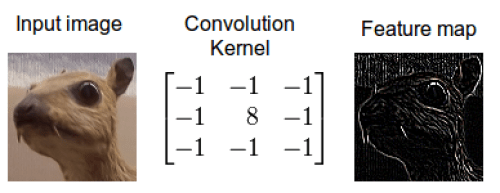
\includegraphics[scale=0.7]{images/ch3/edge-detection.png}
	\caption{Example of a convolution kernel for edge detection}
	\label{fig:edge-detection}
\end{figure}

\subsubsection{Padding}

In the previous example, our input had a height and width of 3 and a convolution kernel with a height and width of 2, yielding an output with a height and a width of 2. In general, assuming the input shape is  $n_h \times n_w$  and the convolution kernel window shape is $k_h \times k_w$, then the output shape will be

$$(n_h-k_h+1) \times (n_w-k_w+1)$$
 
Therefore, the output shape of the convolutional layer is determined by the shape of the input and the shape of the convolution kernel window.

In several cases we might want to incorporate particular techniques --padding and strides-- regarding the size of the output:
\begin{itemize}
    \item In general, since kernels generally have width and height greater than 1, that means that after applying many successive convolutions, we will wind up with an output that is much smaller than our input. If we start with a $240\times240$ pixel image, 10 layers of $5\times5$ convolutions reduce the image to $200\times200$ pixels, slicing off 30\% of the image and with it obliterating any interesting information on the boundaries of the original image. Padding handles this issue.
    \item In some cases, we want to reduce the resolution drastically if say we find our original input resolution to be unwieldy. Strides can help in these instances.
\end{itemize}

\begin{figure}[hpt]
	\centering
	\includesvg{images/ch3/conv_pad.svg}
	\caption{Two-dimensional cross-correlation with padding. The shaded portions are the input and kernel array elements used by the first output element: $0\times0+0\times1+0\times2+0\times3=0$}
	\label{fig:conv_pad}
\end{figure}

In general, if we add a total of  $p_h$  rows of padding (roughly half on top and half on bottom) and a total of  $p_w$  columns of padding (roughly half on the left and half on the right), the output shape will be

$$(n_h-k_h+p_h+1)\times(n_w-k_w+p_w+1)$$
 
This means that the height and width of the output will increase by  $p_h$  and  $p_w$  respectively.

In many cases, we will want to set  $p_h=k_h-1$  and  $p_w=k_w-1$  to give the input and output the same height and width. This will make it easier to predict the output shape of each layer when constructing the network. Assuming that  $k_h$  is odd here, we will pad  $p_h/2$ rows on both sides of the height. If $k_h$  is even, one possibility is to pad  $\lceil p_h/2\rceil$  rows on the top of the input and  $\lfloor p_h/2\rfloor$  rows on the bottom. We will pad both sides of the width in the same way.

ConvNets commonly use correlation kernels with odd height and width values, such as 1, 3, 5, or 7. Choosing odd kernel sizes has the benefit that we can preserve the spatial dimensionality while padding with the same number of rows on top and bottom, and the same number of columns on left and right.

Moreover, this practice of using odd kernels and padding to precisely preserve dimensionality offers a clerical benefit. For any two-dimensional array $X$, when the kernels size is odd and the number of padding rows and columns on all sides are the same, producing an output with the same height and width as the input, we know that the output $Y[i,j]$ is calculated by cross-correlation of the input and convolution kernel with the window centered on $X[i,j]$.

In the following example, we create a two-dimensional convolutional layer with a height and width of 3 and apply 1 pixel of padding on all sides. Given an input with a height and width of 8, we find that the height and width of the output is also 8.

\subsubsection{Stride}

When computing the cross-correlation, we start with the convolution window at the top-left corner of the input array, and then slide it over all locations both down and to the right. In previous examples, we default to sliding one pixel at a time. However, sometimes, either for computational efficiency or because we wish to downsample, we move our window more than one pixel at a time, skipping the intermediate locations.

We refer to the number of rows and columns traversed per slide as the stride. So far, we have used strides of 1, both for height and width. Sometimes, we may want to use a larger stride. The figure below shows a two-dimensional cross-correlation operation with a stride of 3 vertically and 2 horizontally. We can see that when the second element of the first column is output, the convolution window slides down three rows. The convolution window slides two columns to the right when the second element of the first row is output. When the convolution window slides two columns to the right on the input, there is no output because the input element cannot fill the window (unless we add padding).

\begin{figure}[hpt]
	\centering
	\includesvg{images/ch3/conv_stride.svg}
	\caption{Cross-correlation with strides of 3 and 2 for height and width respectively. The shaded portions are the output element and the input and core array elements used in its computation: $0\times0+0\times1+1\times2+2\times3=8,  0\times0+6\times1+0\times2+0\times3=6$}
	\label{fig:conv_stride}
\end{figure}

In general, when the stride for the height is $s_h4  and the stride for the width is s_w$ , the output shape is

$$\lfloor(n_h-k_h+p_h+s_h)/s_h\rfloor \times \lfloor(n_w-k_w+p_w+s_w)/s_w\rfloor$$
 
If we set $p_h=k_h-1$  and  $p_w=k_w-1$ , then the output shape will be simplified to $\lfloor(n_h+s_h-1)/s_h\rfloor \times \lfloor(n_w+s_w-1)/s_w\rfloor$. Going a step further, if the input height and width are divisible by the strides on the height and width, then the output shape will be $(n_h/s_h)\times(n_w/s_w)$.

For the sake of brevity, when the padding number on both sides of the input height and width are $p_h$  and $p_w$  respectively, we call the padding $(p_h,p_w)$. Specifically, when  $p_h=p_w=p$, the padding is $p$. When the strides on the height and width are $s_h$ and $s_w$, respectively, we call the stride $(s_h,s_w)$. Specifically, when $s_h=s_w=s$, the stride is $s$. By default, the padding is 0 and the stride is 1. In practice we rarely use inhomogeneous strides or padding, i.e., we usually have $p_h=p_w$ and $s_h=s_w$.

\subsubsection{Multiple Input and Output Channels}

While we have described the multiple channels that comprise each image (e.g. color images have the standard RGB channels to indicate the amount of red, green and blue), until now, we simplified all of our numerical examples by working with just a single input and a single output channel. This has allowed us to think of our inputs, convolutional kernels, and outputs each as two-dimensional arrays.

When we add channels into the mix, our inputs and hidden representations both become three-dimensional arrays. For example, each RGB input image has shape $3\times h\times w$. We refer to this axis, with a size of 3, as the channel dimension. In this section, we will take a deeper look at convolution kernels with multiple input and multiple output channels.

\paragraph{Multiple Input Channels}

When the input data contains multiple channels, we need to construct a convolution kernel with the same number of input channels as the input data, so that it can perform cross-correlation with the input data. Assuming that the number of channels for the input data is $c_i$, the number of input channels of the convolution kernel also needs to be $c_i$. If our convolution kernel’s window shape is $k_h\times k_w$, then when $c_i=1$, we can think of our convolution kernel as just a two-dimensional array of shape $k_h\times k_w$.

However, when $c_i>1$, we need a kernel that contains an array of shape $k_h\times k_w$ for each input channel. Concatenating these $c_i$ arrays together yields a convolution kernel of shape $c_i\times k_h\times k_w$. Since the input and convolution kernel each have $c_i$ channels, we can perform a cross-correlation operation on the two-dimensional array of the input and the two-dimensional kernel array of the convolution kernel for each channel, adding the $c_i$ results together (summing over the channels) to yield a two-dimensional array. This is the result of a two-dimensional cross-correlation between multi-channel input data and a multi-input channel convolution kernel.

In the figure below, we demonstrate an example of a two-dimensional cross-correlation with two input channels. The shaded portions are the first output element as well as the input and kernel array elements used in its computation:

$$(1 \times 1+2\times2+4\times3+5\times4)+(0\times0+1 \times 1+3\times2+4\times3)=56$$

\begin{figure}[hpt]
	\centering
	\includesvg{images/ch3/conv_multi_in.svg}
	\caption{Cross-correlation computation with 2 input channels. The shaded portions are the first output element as well as the input and kernel array elements used in its computation:  $(1 \times 1+2 \times 2+4\times3+5\times4)+(0\times0+1 \times 1+3\times2+4\times3)=56.$}
	\label{fig:conv_multi_in}
\end{figure}

\paragraph{Multiple Output Channels}

Regardless of the number of input channels, so far we always ended up with one output channel. However, as we discussed earlier, it turns out to be essential to have multiple channels at each layer. In the most popular neural network architectures, we actually increase the channel dimension as we go higher up in the neural network, typically downsampling to trade off spatial resolution for greater channel depth. Intuitively, you could think of each channel as responding to some different set of features. Reality is a bit more complicated than the most naive intepretations of this intuition since representations are not learned independently but are rather optimized to be jointly useful. So it may not be that a single channel learns an edge detector but rather that some direction in channel space corresponds to detecting edges.

Denote by $c_i$ and $c_o$  the number of input and output channels, respectively, and let $k_h$ and $k_w$ be the height and width of the kernel. To get an output with multiple channels, we can create a kernel array of shape $c_i \times k_h \times k_w$ for each output channel. We concatenate them on the output channel dimension, so that the shape of the convolution kernel is $c_o \times c_i \times k_h \times k_w$. In cross-correlation operations, the result on each output channel is calculated from the convolution kernel corresponding to that output channel and takes input from all channels in the input array.

\paragraph{$1 \times 1$ convolutional layers}

At first, a $1 \times 1$  convolution, i.e.  $k_h=k_w=1$, does not seem to make much sense. After all, a convolution correlates adjacent pixels. A $1 \times 1$ convolution obviously does not. Nonetheless, they are popular operations that are sometimes included in the designs of complex deep networks. Let’s see in some detail what it actually does.

Because the minimum window is used, the $1 \times 1$ convolution loses the ability of larger convolutional layers to recognize patterns consisting of interactions among adjacent elements in the height and width dimensions. The only computation of the $1 \times 1$ convolution occurs on the channel dimension.

\cref{fig:conv_1x1} shows the cross-correlation computation using the $1 \times 1$ convolution kernel with 3 input channels and 2 output channels. Note that the inputs and outputs have the same height and width. Each element in the output is derived from a linear combination of elements at the same position in the input image. You could think of the $1 \times 1$  convolutional layer as constituting a fully-connected layer applied at every single pixel location to transform the $c_i$ corresponding input values into $c_o$ output values. Because this is still a convolutional layer, the weights are tied across pixel location Thus the $1 \times 1$  convolutional layer requires $c_o \times c_i$ weights (plus the bias terms).

\begin{figure}[hpt]
	\centering
	\includesvg{images/ch3/conv_1x1.svg}
	\caption{Cross-correlation computation using a $1 \times 1$ convolution kernel with 3 input channels and 2 output channels. The inputs and outputs have the same height and width.}
	\label{fig:conv_1x1}
\end{figure}

\subsection{Pooling layers}\label{subsec:pool_layers}

Often, as we process images, we want to gradually reduce the spatial resolution of our hidden representations, aggregating information so that the higher up we go in the network, the larger the receptive field (in the input) to which each hidden node is sensitive.

Often our ultimate task asks some global question about the image, e.g., does it contain a cat? So typically the nodes of our final layer should be sensitive to the entire input. By gradually aggregating information, yielding coarser and coarser maps, we accomplish this goal of ultimately learning a global representation, while keeping all of the advantages of convolutional layers at the intermediate layers of processing.

Moreover, when detecting lower-level features, such as edges, we often want our representations to be somewhat invariant to translation. For instance, if we take the image X with a sharp delineation between black and white and shift the whole image by one pixel to the right, i.e. $Z[i,j] = X[i,j+1]$ then the output for for the new image Z might be vastly different. The edge will have shifted by one pixel and with it all the activations. In reality, objects hardly ever occur exactly at the same place. In fact, even with a tripod and a stationary object, vibration of the camera due to the movement of the shutter might shift everything by a pixel or so.

Pooling layers serve the dual purposes of mitigating the sensitivity of convolutional layers to location and of spatially downsampling representations.

\subsubsection{Maximum Pooling and Average Pooling}

Like convolutional layers, pooling layers apply a fixed-shape window that slides over all regions in the input according to its stride, computing a single output for each location traversed by the fixed-shape window (sometimes known as the pooling window). However, unlike convolutional layers, which need parameters to represent the correlation kernels, the pooling layer contains no parameters (there is no kernel). Instead, pooling operators are deterministic, typically calculating either the maximum or the average value of the elements in the pooling window. These operations are called maximum pooling (\textit{max pooling} for short) and \textit{average pooling}, respectively.

In both cases, as with the cross-correlation operator, we can think of the pooling window as starting from the top left of the input array and sliding across the input array from left to right and top to bottom. At each location that the pooling window hits, it computes the maximum or average value of the input subarray in the window (depending on whether max or average pooling is employed).

\begin{figure}[hpt]
	\centering
	\includesvg{images/ch3/pooling.svg}
	\caption{Maximum pooling with a pooling window shape of $2\times2$. The shaded portions represent the first output element and the input element used for its computation:  $\max(0,1,3,4)=4$.}
	\label{fig:pooling}
\end{figure}

The output array in \cref{fig:pooling} has a height of 2 and a width of 2. The four elements are derived from the maximum value of $\text{max}$:

\begin{align*}
\max(0,1,3,4)=4,\\
\max(1,2,4,5)=5,\\
\max(3,4,6,7)=7,\\
\max(4,5,7,8)=8.\\
\end{align*}

A pooling layer with a pooling window shape of $p \times q$ is called a $p \times q$ pooling layer. The pooling operation is called $p \times q$ pooling.

Let us return to the object edge detection example mentioned at the beginning of this section. Now we will use the output of the convolutional layer as the input for $2 \times 2$  max pooling. Set the convolutional layer input as $X$ and the pooling layer output as $Y$. Whether or not the values of $X[i, j]$ and $X[i, j+1]$ are different, or $X[i, j+1]$ and $X[i, j+2]$ are different, the pooling layer outputs all include $Y[i, j]=1$. That is to say, using the $2 \times 2$ maximum pooling layer, we can still detect if the pattern recognized by the convolutional layer moves no more than one element in height and width.

\subsubsection{Padding and Stride}

As with convolutional layers, pooling layers can also change the output shape. And as before, we can alter the operation to achieve a desired output shape by padding the input and adjusting the stride.

When processing multi-channel input data, the pooling layer pools each input channel separately, rather than adding the inputs of each channel by channel as in a convolutional layer. This means that the number of output channels for the pooling layer is the same as the number of input channels

% \subsection{Summary of ConvNets}

% \begin{itemize}
%     \item Translation invariance in images implies that all patches of an image will be treated in the same manner.
%     \item Locality means that only a small neighborhood of pixels will be used for computation.    
%     \item Channels on input and output allows for meaningful feature analysis.
%     \item The core computation of a two-dimensional convolutional layer is a two-dimensional cross-correlation operation. In its simplest form, this performs a cross-correlation operation on the two-dimensional input data and the kernel, and then adds a bias.
%     \item We can design a kernel to detect edges in images.
%     \item We can learn the kernel through data
%     \item Padding can increase the height and width of the output. This is often used to give the output the same height and width as the input.
%     \item The stride can reduce the resolution of the output, for example reducing the height and width of the output to only  $1/n$  of the height and width of the input ($n$  is an integer greater than 1)
%     \item Padding and stride can be used to adjust the dimensionality of the data effectively.
%     \item Multiple channels can be used to extend the model parameters of the convolutional layer.
%     \item The $1 \times 1$ convolutional layer is equivalent to the fully-connected layer, when applied on a per pixel basis.
%     \item The $1 \times 1$  convolutional layer is typically used to adjust the number of channels between network layers and to control model complexity.
%     \item Taking the input elements in the pooling window, the maximum pooling operation assigns the maximum value as the output and the average pooling operation assigns the average value as the output.
%     \item One of the major functions of a pooling layer is to alleviate the excessive sensitivity of the convolutional layer to location.
%     \item We can specify the padding and stride for the pooling layer.
%     \item Maximum pooling, combined with a stride larger than 1 can be used to reduce the resolution.
%     \item The pooling layer’s number of output channels is the same as the number of input channels.
% \end{itemize}

\subsection{Examples of concrete CNN architectures}

\subsubsection{Classical convolutional networks: LeNet}

In this section, we will introduce one of the first published convolutional neural networks whose benefit was first demonstrated by  \citet{Lecun1998}, for the purpose of recognizing handwritten digits in images. In the 90s, their experiments with \href{LeNet}{http://yann.lecun.com/exdb/lenet/} gave the first compelling evidence that it was possible to train convolutional neural networks by backpropagation. Their model achieved outstanding results at the time (only matched by Support Vector Machines at the time) and was adopted to recognize digits for processing deposits in ATM machines. Some ATMs still runn the code that Yann and his colleague Leon Bottou wrote in the 1990s.

In a rough sense, we can think LeNet as consisting of two parts: (i) a block of convolutional layers; and (ii) a block of fully-connected layers. Before getting into the weeds, let’s briefly review the model in \cref{fig:letnet}

\begin{figure}[hpt]
	\centering
	\includesvg[scale=0.4]{images/ch3/lenet.svg}
	\caption{Data flow in LeNet 5. The input is a handwritten digit, the output a probabilitiy over 10 possible outcomes.}
	\label{fig:lenet}
\end{figure}

The basic units in the convolutional block are a convolutional layer and a subsequent average pooling layer (note that max-pooling works better, but it had not been invented in the 90s yet). The convolutional layer is used to recognize the spatial patterns in the image, such as lines and the parts of objects, and the subsequent average pooling layer is used to reduce the dimensionality. The convolutional layer block is composed of repeated stacks of these two basic units. Each convolutional layer uses a $5 \times 5$  kernel and processes each output with a \textit{sigmoid} activation function (again, note that \textit{ReLU}s are now known to work more reliably, but had not been invented yet). The first convolutional layer has 6 output channels, and second convolutional layer increases channel depth further to 16.

However, coinciding with this increase in the number of channels, the height and width are shrunk considerably. Therefore, increasing the number of output channels makes the parameter sizes of the two convolutional layers similar. The two average pooling layers are of size  $2 \times 2$  and take stride 2 (note that this means they are non-overlapping). In other words, the pooling layer downsamples the representation to be precisely one quarter the pre-pooling size.

The convolutional block emits an output with size given by (batch size, channel, height, width). Before we can pass the convolutional block’s output to the fully-connected block, we must flatten each example in the mini-batch. In other words, we take this 4D input and transform it into the 2D input expected by fully-connected layers: as a reminder, the first dimension indexes the examples in the mini-batch and the second gives the flat vector representation of each example. LeNet’s fully-connected layer block has three fully-connected layers, with 120, 84, and 10 outputs, respectively. Because we are still performing classification, the 10 dimensional output layer corresponds to the number of possible output classes.

Summing up: 
\begin{itemize}
    \item A convolutional neural network (in short, ConvNet) is a network using convolutional layers.
    \item In a ConvNet we alternate between convolutions, nonlinearities and often also pooling operations.
    \item Ultimately the resolution is reduced prior to emitting an output via one (or more) dense layers.
    \item LeNet was the first successful deployment of such a network.
\end{itemize}

\subsubsection{Modern architectures}

Although convolutional neural networks were well known in the computer vision and machine learning communities following the introduction of LeNet, they did not immediately dominate the field. Although LeNet achieved good results on early small data sets, the performance and feasibility of training convolutional networks on larger, more realistic datasets had yet to be established
In fact, for much of the intervening time between the early 1990s and the watershed results of 2012, neural networks were often surpassed by other machine learning methods, such as support vector machines.

A major breakthrough came when Alex Krizhevsky and Ilya Sutskever implemented a deep convolutional neural network that could run on GPU hardware. They realized that the computational bottlenecks in CNNs (convolutions and matrix multiplications) are all operations that could be parallelized in hardware. Using two NIVIDA GTX 580s with 3GB of memory, they implemented fast convolutions. The code \href{https://code.google.com/archive/p/cuda-convnet/}{cuda-convnet} was good enough that for several years it was the industry standard and powered the first couple years of the deep learning boom.

\paragraph{AlexNet: first large-scale convnet, beating classical methods in computer vision}


AlexNet was introduced in 2012, named after Alex Krizhevsky, the first author of the breakthrough ImageNet classification paper \citep{Krizhevsky2012}. AlexNet, which employed an 8-layer convolutional neural network, won the ImageNet Large Scale Visual Recognition Challenge 2012 by a phenomenally large margin. This network proved, for the first time, that the features obtained by learning can transcend manually-design features, breaking the previous paradigm in computer vision. The architectures of AlexNet and LeNet are \textit{very similar}, as the diagram below illustrates. Note that we provide a slightly streamlined version of AlexNet removing some of the design quirks that were needed in 2012 to make the model fit on two small GPUs.

\begin{figure}[hpt]
	\centering
	\includesvg[scale=0.8]{images/ch3/alexnet-all.svg}
	\caption{LeNet (left) and AlexNet (right)}
	\label{fig:alexnet}
\end{figure}

The design philosophies of AlexNet and LeNet are very similar, but there are also significant differences. First, AlexNet is much deeper than the comparatively small LeNet5. AlexNet consists of eight layers: five convolutional layers, two fully-connected hidden layers, and one fully-connected output layer. Second, AlexNet used the ReLU instead of the sigmoid as its activation function.

\paragraph{VGG: network architecture based on repeating blocks}

While AlexNet proved that deep convolutional neural networks can achieve good results, it didn't offer a general template to guide subsequent researchers in designing new networks.  In the following sections, we will introduce several heuristic concepts commonly used to design deep networks.

Progress in this field mirrors that in chip design where engineers went from placing transistors to logical elements to logic blocks. Similarly, the design of neural network architectures  had grown progressively more abstract, with researchers moving from thinking in terms of individual neurons to whole layers, and now to blocks, repeating patterns of layers.

The idea of using blocks first emerged from the \href{http://www.robots.ox.ac.uk/~vgg/}{Visual Geometry Group} (VGG) at Oxford University. In their eponymously-named VGG network, It's easy to implement these repeated structures in code with any modern deep learning framework by using loops and subroutines. 

The basic building block of classic convolutional networks is a sequence of the following layers: (i) a convolutional layer  (with padding to maintain the resolution), (ii) a nonlinearity such as a ReLu.

One VGG block consists of a sequence of convolutional layers,  followed by a max pooling layer for spatial downsampling. In the original VGG paper \citet{Simonyan2015} employed convolutions with $3\times3$ kernels and $2 \times 2$ max pooling with stride of $2$ (halving the resolution after each block).

Like AlexNet and LeNet, the VGG Network can be partitioned into two parts: the first consisting mostly of convolutional and pooling layers and a second consisting of fully-connected layers. The convolutional portion of the net connects several \textit{vgg block} modules in succession.

\begin{figure}[hpt]
	\centering
	\includesvg[scale=0.8]{images/ch3/vgg.svg}
	\caption{Designing a network from building blocks}
	\label{fig:vgg}
\end{figure}

The original VGG network had 5 convolutional blocks, among which the first two have one convolutional layer each and the latter three contain two convolutional layers each. The first block has 64 output channels and each subsequent block doubles the number of output channels, until that number reaches $512$. Since this network uses $8$ convolutional layers and $3$ fully-connected layers, it is often called VGG-11.

\paragraph{GoogleLeNet (aka Inception): using parallel concatenations}

\paragraph{ResNet: residual networks}

\paragraph{DenseNet: densely connected architecture}


\section{Recurrent Neural Networks}\label{sec:rnn}

So far we encountered two types of data: generic vectors and images. For the latter we designed specialized layers to take advantage of the regularity properties in them. Besides, we tacitly assumed that our data is generated i.i.d., i.e. independently and identically distributed, all drawn from some distribution. Unfortunately, this is not true for many types of data. For instance, the words in this paragraph are written in sequence, and it would be quite difficult to decipher its meaning if they were permuted randomly. Likewise, image frames in a video, the audio signal in a conversation, or the browsing behavior on a website, all follow sequential order. It is thus only reasonable to assume that specialized models for such data will do better at describing it and at solving estimation problems.

Another issue arises from the fact that we might not only receive a sequence as an input but rather might be expected to continue the sequence. For instance, the task could be to continue the series 2, 4, 6, 8, 10, … This is quite common in time series analysis, to predict the stock market, the fever curve of a patient or the acceleration needed for a race car. Again we want to have models that can handle such data.

In short, while convolutional neural networks can efficiently process spatial information, recurrent neural networks are designed to better handle sequential information. These networks introduces state variables to store past information and, together with the current input, determine the current output.

Many of the examples for using recurrent networks are based on text data. Hence, we will emphasize language models in this chapter. After a more formal review of sequence data we discuss basic concepts of a language model and use this discussion as the inspiration for the design of recurrent neural networks. Next, we describe the gradient calculation method in recurrent neural networks to explore problems that may be encountered in recurrent neural network training. For some of these problems, we can use gated recurrent neural networks, such as LSTMs and GRUs, described later in this section.

\subsection{Sequence models}\label{subsec:sequence_models}

There many examples of observable behaviour and phenomena that are sequential in nature, that is, that change over time. In mathematics, a sequence is a list of objects (or events) which have been fully ordered, such that each member either comes before, or after, every other member. More formally, a sequence is a function with a domain equal to the set of positive integers.

In short, we need statistical tools and new deep networks architectures to deal with sequence data. To keep things simple, we use stock prices as an example (see \cref{fig:ftse100}).

\begin{figure}[hpt]
	\centering
	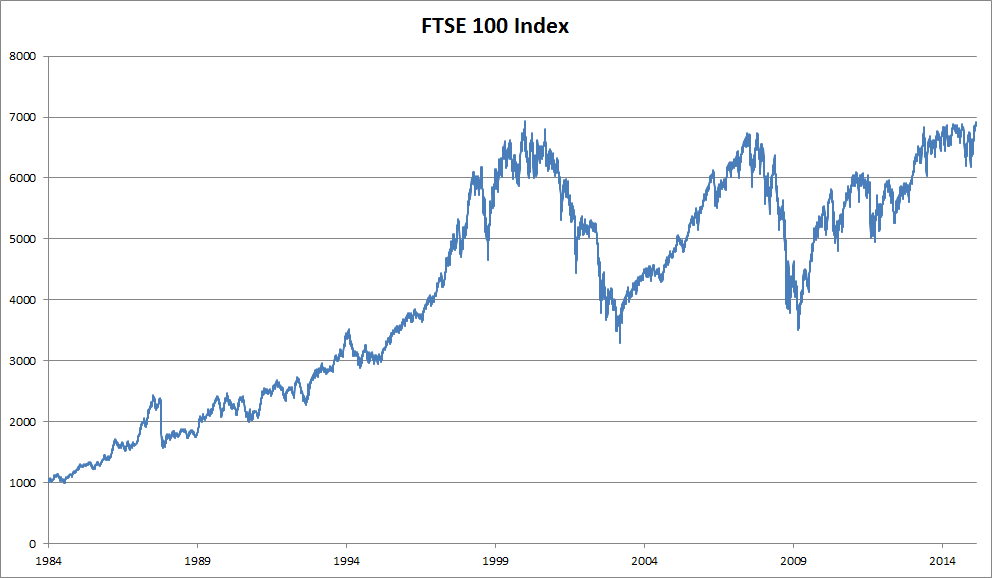
\includegraphics[scale=0.5]{images/ch3/ftse100.png}
	\caption{FTSE 100 index over 30 years.}
	\label{fig:ftse100}
\end{figure}

Let’s denote the prices by $x_t \geq 0$, i.e. at time $t \in \mathbb{N}$ we observe some price $x_t$. For a trader to do well in the stock market on day $t$ he should want to predict $x_t$ via

$$x_t \sim p(x_t|x_{t-1}, \ldots x_1)$$

\subsubsection{Autoregressive Models}

In order to achieve this, our trader could use a regressor, but there’s just a major problem - the number of inputs, $x_{t-1}, \ldots x_1$ varies, depending on $t$. That is, the number increases with the amount of data that we encounter, and we will need an approximation to make this computationally tractable. Much of what follows in this section will revolve around how to estimate $p(x_t|x_{t-1}, \ldots x_1)$ efficiently. In a nutshell it boils down to two strategies:

\begin{enumerate}
    \item Assume that the potentially rather long sequence $x_{t-1}, \ldots x_1$ is not really necessary. In this case we might content ourselves with some timespan $\tau$ and only use $x_{t-1}, \ldots x_{t-\tau}$ observations. The immediate benefit is that now the number of arguments is always the same, at least for $t > \tau$. This allows us to train a deep network as indicated above. Such models will be called \textit{autoregressive models}, as they quite literally perform regression on themselves.
    \item Another strategy is to try and keep some summary $h_t$ of the past observations around and update that in addition to the actual prediction. This leads to models that estimate $x_t|x_{t-1}, h_{t-1}$ and moreover updates of the form $h_t = g(h_t, x_t)$. Since $h_t$ is never observed, these models are also called \textit{latent autoregressive models}. LSTMs and GRUs are examples of this.
\end{enumerate}

Both cases raise the obvious question of how to generate training data. One typically uses historical observations to predict the next observation given the ones up to right now. Obviously we do not expect time to stand still. However, a common assumption is that while the specific values of $x_t$ might change, at least the dynamics of the time series itself won’t. This is reasonable, since novel dynamics are just that, novel and thus not predictable using data we have so far. Statisticians call dynamics that do not change stationary. Regardless of what we do, we will thus get an estimate of the entire time series via

$$p(x_1, \ldots x_T) = \prod_{t=1}^T p(x_t|x_{t-1}, \ldots x_1)$$

Note that the above considerations still hold if we deal with discrete objects, such as words, rather than numbers. The only difference is that in such a situation we need to use a classifier rather than a regressor to estimate $p(x_t| x_{t-1}, \ldots x_1)$.

\subsubsection{Markov Model}

Recall the approximation that in an autoregressive model we use only $(x_{t-1}, \ldots x_{t-\tau})$ instead of $(x_{t-1}, \ldots x_1)$ to estimate $x_t$. Whenever this approximation is accurate we say that the sequence satisfies a Markov condition. In particular, if $\tau = 1$, we have a first order Markov model and $p(x)$ is given by

$$p(x_1, \ldots x_T) = \prod_{t=1}^T p(x_t|x_{t-1})$$

Such models are particularly nice whenever $x_t$ assumes only discrete values, since in this case dynamic programming can be used to compute values along the chain exactly. For instance, we can compute $x_{t+1}|x_{t-1}$ efficiently using the fact that we only need to take into account a very short history of past observations.

$$p(x_{t+1}|x_{t-1}) = \sum_{x_t} p(x_{t+1}|x_t) p(x_t|x_{t-1})$$

Going into details of dynamic programming is beyond the scope of this section. Control and reinforcement learning algorithms use such tools extensively.

\subsubsection{Causality}

In principle, there’s nothing wrong with unfolding $p(x_1, \ldots x_T)$ in reverse order. After all, by conditioning we can always write it via

$$p(x_1, \ldots x_T) = \prod_{t=T}^1 p(x_t|x_{t+1}, \ldots x_T)$$

In fact, if we have a Markov model we can obtain a reverse conditional probability distribution, too. In many cases, however, there exists a natural direction for the data, namely going forward in time. It is clear that future events cannot influence the past. Hence, if we change $x_t$, we may be able to influence what happens for $x_{t+1}$ going forward but not the converse. That is, if we change $x_t$, the distribution over past events will not change. Consequently, it ought to be easier to explain $x_{t+1}|x_t$ rather than $x_t|x_{t+1}$. For instance, \citet{Hoyer2008} show that in some cases we can find $x_{t+1} = f(x_t) + \epsilon$ for some additive noise, whereas the converse is not true. This is great news, since it is typically the forward direction that we’re interested in estimating. For more on this topic see for example the book \textit{Elements of Causal Inference}, by \citet{Peters2015}; we are barely scratching the surface of it.

\subsection{Language models}\label{subsec:lang_models}

Text is an important example of sequence data. In fact, we will use natural language models as the basis for many of the examples in this chapter. Given that, it’s worth while discussing some things in a bit more detail. In the following we will view words (or sequences of characters) as a time series of discrete observations. Assuming the words in a text of length $T$ are in turn $w_1, w_2, \ldots, w_T$, then, in the discrete time series, $w_t(1 \leq t \leq T)$ can be considered as the output or label of time step $t$. Given such a sequence, the goal of a language model is to estimate the probability

$$p(w_1, w_2, \ldots, w_T)$$

Language models are incredibly useful. For instance, an ideal language model would be able to generate natural text just on its own, simply by drawing one word at a time $w_t \sim p(w_t|w_{t-1}, \ldots w_1)$. Quite unlike the monkey using a typewriter, all text emerging from such a model would pass as natural language, e.g. English text. Furthermore, it would be sufficient for generating a meaningful dialog, simply by conditioning the text on previous dialog fragments. Clearly we are still very far from designing such a system, since it would need to understand the text rather than just generate grammatically sensible content.

Nonetheless language models are of great service even in their limited form. For instance, the phrases ‘to recognize speech’ and ‘to wreck a nice beach’ sound very similar. This can cause ambiguity in speech recognition, ambiguity that is easily resolved through a language model which rejects the second translation as outlandish. Likewise, in a document summarization algorithm it’s worth while knowing that ‘dog bites man’ is much more frequent than ‘man bites dog’, or that ‘let’s eat grandma’ is a rather disturbing statement, whereas ‘let’s eat, grandma’ is much more benign.

\subsubsection{Estimating a language model}

The obvious question is how we should model a document, or even a sequence of words. We can start by applying basic probability rules:

$$p(w_1, w_2, \ldots, w_T) = \prod_{t=1}^T p(w_t | w_1, \ldots, w_{t-1})$$

For example, the probability of a text sequence containing four tokens consisting of words and punctuation would be given as:

$$p(\mathrm{Statistics}, \mathrm{is},  \mathrm{fun}, \mathrm{.}) =  p(\mathrm{Statistics}) p(\mathrm{is} | \mathrm{Statistics}) p(\mathrm{fun} | \mathrm{Statistics}, \mathrm{is}) p(\mathrm{.} | \mathrm{Statistics}, \mathrm{is}, \mathrm{fun})$$

In order to compute the language model, we need to calculate the probability of words and the conditional probability of a word given the previous few words, i.e. language model parameters. Here, we assume that the training data set is a large text corpus, such as all Wikipedia entries, Project Gutenberg, or all text posted online on the web. The probability of words can be calculated from the relative word frequency of a given word in the training data set.

For example, $p(\mathrm{Statistics})$ can be calculated as the probability of any sentence starting with the word ‘statistics’. A slightly less accurate approach would be to count all occurrences of the word ‘statistics’ and divide it by the total number of words in the corpus. This works fairly well, particularly for frequent words. Moving on, we could attempt to estimate

$$\hat{p}(\mathrm{is}|\mathrm{Statistics}) = \frac{n(\mathrm{Statistics~is})}{n(\mathrm{Statistics})}$$

Here $n(w)$ and $n(w, w')$ are the number of occurrences of singletons and pairs of words respectively. Unfortunately, estimating the probability of a word pair is somewhat more difficult, since the occurrences of ‘Statistics is’ are a lot less frequent. In particular, for some unusual word combinations it may be tricky to find enough occurrences to get accurate estimates. Things take a turn for the worse for 3 word combinations and beyond. There will be many plausible 3-word combinations that we likely will not see in our dataset. Unless we provide some solution to give such word combinations nonzero weight we will not be able to use these as a language model. If the dataset is small or if the words are very rare, we might not find even a single one of them.

A common strategy is to perform some form of Laplace smoothing, that is, adding a small constant to all counts. 
%This helps with singletons, e.g. via

% $$
% \begin{aligned}
%     \hat{p}(w) & = \frac{n(w) + \epsilon_1/m}{n + \epsilon_1} \\
%     \hat{p}(w'|w) & = \frac{n(w,w') + \epsilon_2 \hat{p}(w')}{n(w) + \epsilon_2} \\
%     \hat{p}(w''|w',w) & = \frac{n(w,w',w'') + \epsilon_3 \hat{p}(w',w'')}{n(w,w') + \epsilon_3}
% \end{aligned}
% $$

% Here the coefficients $\epsilon_i > 0$ determine how much we use the estimate for a shorter sequence as a fill-in for longer ones. Moreover, $m$ is the total number of words we encounter. The above is a rather primitive variant of what Kneser-Ney smoothing and Bayesian Non-parametrics can accomplish. 

See e.g. \textit{The Sequence Memoizer} by \citep{Wood2011} for more details of how to accomplish this. Unfortunately models like this get unwieldy rather quickly. First off, we need to store all counts and secondly, this entirely ignores the meaning of the words; for instance, ‘cat’ and ‘feline’ should occur in related contexts. Besides, it is quite difficult to adjust such models to additional context. Lastly, long word sequences are almost certain to be novel, hence a model that simply counts the frequency of previously seen word sequences is bound to perform poorly there.

\subsubsection{Markov Models and n-grams}

Before we discuss solutions involving deep learning we need some more terminology and concepts. Recall our discussion of Markov Models in the previous section. Let’s apply this to language modeling. A distribution over sequences satisfies the Markov property of first order if $p(w_{t+1}|w_t, \ldots w_1) = p(w_{t+1}|w_t)$. Higher orders correspond to longer dependencies. This leads to a number of approximations that we could apply to model a sequence:

$$
\begin{aligned}
p(w_1, w_2, w_3, w_4) &=  p(w_1) p(w_2) p(w_3) p(w_4)\\
p(w_1, w_2, w_3, w_4) &=  p(w_1) p(w_2 | w_1) p(w_3 | w_2) p(w_4 | w_3)\\
p(w_1, w_2, w_3, w_4) &=  p(w_1) p(w_2 | w_1) p(w_3 | w_1, w_2) p(w_4 | w_2, w_3)\\
\end{aligned}
$$

Since they involve one, two or three terms, these are typically referred to as \textit{unigram}, \textit{bigram} and \textit{trigram} models. 
% In the following we will learn how to design better models.

\subsection{Recurrent Neural Networks}\label{subsec:rnn}

In the previous section we introduced $n$-gram models, where the conditional probability of word $w_t$ at position $t$ only depends on the $n-1$ previous words. If we want to check the possible effect of words earlier than $t-(n-1)$ on $w_t$, we need to increase $n$. However, the number of model parameters would also increase exponentially with it, as we need to store $|V|^n$ numbers for a vocabulary $V$. Hence, rather than modeling $p(w_t|w_{t-1}, \ldots w_{t-n+1})$ it is preferable to use a latent variable model in which we have

$$p(w_t|w_{t-1}, \ldots w_1) \approx p(w_t|h_t(w_{t-1}, h_{t-1})).$$

For a sufficiently powerful function $h_t$ this is not an approximation. After
all, $h_t$ could simply store all the data it observed so far. We discussed this
in \cref{subsec:sequence_models}. Let's see why building such models is a bit more tricky than simple autoregressive models where

$$p(w_t|w_{t-1}, \ldots w_1) \approx p(w_t|f(w_{t-1}, \ldots w_{t-n+1}))$$

As a warmup we will review the latter for discrete outputs and $n=2$, i.e. for Markov model of first order. To simplify things further we use a single layer in the design of the RNN. Later on we will see how to add more expressivity efficiently across items.

\subsubsection{Recurrent Networks Without Hidden States}

Let us take a look at a multilayer perceptron with a single hidden layer. Given a mini-batch of instances $\mathbf{X} \in \mathbb{R}^{n \times d}$ with sample size $n$ and $d$ inputs (features or feature vector dimensions). Let the hidden layer's activation function be $\phi$. Hence the hidden layer's output $\mathbf{H} \in \mathbb{R}^{n \times h}$ is calculated as

$$\mathbf{H} = \phi(\mathbf{X} \mathbf{W}_{xh} + \mathbf{b}_h).$$

Here, we have the weight parameter $\mathbf{W}_{xh} \in \mathbb{R}^{d \times h}$, bias parameter $\mathbf{b}_h \in \mathbb{R}^{1 \times h}$, and the number of hidden units $h$, for the hidden layer. 
% Recall that $\mathbf{b}_h$ is just a vector - its values are replicated using the broadcasting mechanism to match those of the matrix-matrix product.

Also note that hidden \textbf{state} and hidden \textbf{layer} refer to two very different concepts. Hidden layers are layers that are hidden from view on the path from input to output. Hidden states are technically speaking inputs to whatever we do at a given step. Instead, they can only be computed by looking at data at previous iterations. In this sense they have much in common with latent variable models in statistics, such as clustering or topic models where e.g. the cluster ID affects the output but cannot be directly observed.

The hidden variable $\mathbf{H}$ is used as the input of the output layer. For classification purposes, such as predicting the next character, the output dimensionality $q$ might e.g. match the number of categories in the classification problem. Lastly the output layer is given by

$$\mathbf{O} = \mathbf{H} \mathbf{W}_{hq} + \mathbf{b}_q.$$

Here, $\mathbf{O} \in \mathbb{R}^{n \times q}$ is the output variable, $\mathbf{W}_{hq} \in \mathbb{R}^{h \times q}$ is the weight parameter, and $\mathbf{b}_q \in \mathbb{R}^{1 \times q}$ is the bias parameter of the output layer.  If it is a classification problem, we can use $\text{softmax}(\mathbf{O})$ to compute the probability distribution of the output category. This is entirely analogous to the regression problem we solved previously in \cref{subsec:sequence_models}, hence we omit details. Suffice it to say that we can pick $(w_t, w_{t-1})$ pairs at random and estimate the parameters $\mathbf{W}$ and $\mathbf{b}$ of our network via autograd and stochastic gradient descent.

\subsubsection{Recurrent Networks with Hidden States}\label{subsubsec:rnn_with_hidden_state}

Matters are entirely different when we have hidden states. Let's look at the structure in some more detail. Assume that $\mathbf{X}_t \in \mathbb{R}^{n \times d}$ is the mini-batch input and $\mathbf{H}_t  \in \mathbb{R}^{n \times h}$ is the hidden variable of time step $t$ from the sequence.  Unlike the multilayer perceptron, here we save the hidden variable $\mathbf{H}_{t-1}$ from the previous time step and introduce a new weight parameter $\mathbf{W}_{hh} \in \mathbb{R}^{h \times h}$, to describe how to use the hidden variable of the previous time step in the current time step. Specifically, the calculation of the hidden variable of the current time step is determined by the input of the current time step together with the hidden variable of the previous time step:

$$\mathbf{H}_t = \phi(\mathbf{X}_t \mathbf{W}_{xh} + \mathbf{H}_{t-1} \mathbf{W}_{hh}  + \mathbf{b}_h)$$

Compared with the multilayer perceptron, we added one more $\mathbf{H}_{t-1} \mathbf{W}_{hh}$ here. From the relationship between hidden variables $\mathbf{H}_t$ and $\mathbf{H}_{t-1}$ of adjacent time steps, we know that those variables captured and retained the sequence's historical information up to the current time step, just like the state or memory of the neural network's current time step. Therefore, such a hidden variable is also called a hidden state. Since the hidden state uses the same definition of the previous time step in the current time step, the computation of the equation above is recurrent, hence the name recurrent neural network (RNN).

There are many different RNN construction methods.  RNNs with a hidden state defined by the equation above are very common. For time step $t$, the output of the output layer is similar to the computation in the multilayer perceptron:

$$\mathbf{O}_t = \mathbf{H}_t \mathbf{W}_{hq} + \mathbf{b}_q$$

RNN parameters include the weight $\mathbf{W}_{xh} \in \mathbb{R}^{d \times h}, \mathbf{W}_{hh} \in \mathbb{R}^{h \times h}$ of the hidden layer with the bias $\mathbf{b}_h \in \mathbb{R}^{1 \times h}$, and the weight $\mathbf{W}_{hq} \in \mathbb{R}^{h \times q}$ of the output layer with the bias $\mathbf{b}_q \in \mathbb{R}^{1 \times q}$. It is worth mentioning that RNNs always use these model parameters, even for different time steps. Therefore, the number of RNN model parameters does not grow as the number of time steps increases.

\cref{fig:rnn} shows the computational logic of an RNN at three adjacent time steps. In time step $t$, the computation of the hidden state can be treated as an entry of a fully connected layer with the activation function $\phi$ after concatenating the input $\mathbf{X}_t$ with the hidden state $\mathbf{H}_{t-1}$ of the previous time step.  The output of the fully connected layer is the hidden state of the current time step $\mathbf{H}_t$. Its model parameter is the concatenation of $\mathbf{W}_{xh}$ and $\mathbf{W}_{hh}$, with a bias of $\mathbf{b}_h$. The hidden state of the current time step $t$ $\mathbf{H}_t$ will participate in computing the hidden state $\mathbf{H}_{t+1}$ of the next time step $t+1$, the result of which will become the input for the fully connected output layer of the current time step.

\begin{figure}[hpt]
	\centering
	\includesvg[scale=0.5]{images/ch3/rnn.svg}
	\caption{An RNN with a hidden state.}
	\label{fig:rnn}
\end{figure}

As discussed, the computation in the hidden state uses $\mathbf{H}_t = \mathbf{X}_t \mathbf{W}_{xh} + \mathbf{H}_{t-1} \mathbf{W}_{hh}$ to generate an object matching $\mathbf{H}_{t-1}$ in dimensionality. Moreover, we use $\mathbf{H}_t$ to generate the output $\mathbf{O}_t = \mathbf{H}_t \mathbf{W}_{hq}$.

The recurrent network defined above takes observations $X$ and a hidden state $H$ as arguments and uses them to update the hidden state and emit an output $O$. Since this chain could go on for a very long time, training the model with backprop is out of the question (at least without some approximation). After all, this leads to a very long chain of dependencies that would be prohibitive to solve exactly: books typically have more than 100,000 characters and it is unreasonable to assume that the later text relies indiscriminately on all occurrences that happened, say, 10,000 characters in the past. Truncation methods such as BPTT and long short term memory, described later, are useful to address this in a more principled manner. 

\subsubsection{Recurrent networks for language modelling}\label{subsubsec:rnn_lang_modelling}

We conclude this section by illustrating how RNNs can be used to build a language model. For simplicity of illustration we use words rather than characters, since the former are easier to comprehend. Let the number of mini-batch examples be 1, and the sequence of the text be the beginning of our dataset, i.e. “The time Machine by H. G. Wells”. \cref{fig:rnn-train} illustrates how to estimate the next character based on the present and previous characters. During the training process, we run a softmax operation on the output from the output layer for each time step, and then use the cross-entropy loss function to compute the error between the result and the label. Due to the recurrent computation of the hidden state in the hidden layer, the output of time step 3, $\mathbf{O}_3$ is determined by the text sequence “the”, “time”, “machine”. Since the next word of the sequence in the training data is “by”, the loss of time step 3 will depend on the probability distribution of the next word generated based on the sequence “the”, “time”, “machine” and the label “by” of this time step.

\begin{figure}[hpt]
	\centering
	\includesvg[scale=0.8]{images/ch3/rnn-train.svg}
	\caption{Word-level RNN language model. The input and label sequences are The Time Machine by H. and Time Machine by H. G. respectively.}
	\label{fig:rnn-train}
\end{figure}


The number of words is huge compared to the number of characters. This is why quite often we will use a character-level RNN instead.

% \subsection{Text Preprocessing}

% \subsubsection{Tokenization and vocabulary building}

% In the previous section we discussed some properties that make language unique. The key is that the number of tokens (aka words) is large and very unevenly distributed. Hence, a naive multiclass classification approach to predict the next symbol doesn’t always work very well. Moreover, we need to turn text into a format that we can optimize over, i.e. we need to map it to vectors. At its extreme we have two alternatives. One is to treat each word as a unique entity, e.g. \citep{Salton1975}. The problem with this strategy is that we might well have to deal with 100,000 to 1,000,000 vectors for very large and diverse corpora.

% At the other extreme lies the strategy to predict one character at a time, as suggested e.g. by \citet{Ling2015}. A good balance in between both strategies is byte-pair encoding, as described by \citet{Sennrich2016} for the purpose of neural machine translation. It decomposes text into syllable-like fragments that occur frequently. This allows for models that are able to generate words like heteroscedastic or pentagram based on previously viewed words, e.g. heterogeneous, homoscedastic, diagram, and pentagon. Going into details of these models is beyond the scope of the current chapter. 

% Next we need to split the dataset, a string, into tokens. A token is a data point the model will train and predict. We commonly use a word or a character as a token.

% Then we need to map tokens into numerical indices. We often call it a vocabulary. Its input is a list of tokens, called a corpus. Then it counts the frequency of each token in this corpus, and then assigns an numerical index to each token according to its frequency. Rarely appeared tokens are often removed to reduce the complexity. A token doesn’t exist in corpus or has been removed is mapped into a special unknown ("<unk>") token. We optionally add another three special tokens: "<pad>" a token for padding, "<bos>" to present the beginning for a sentence, and "<eos>" for the ending of a sentence.

% \subsubsection{Sampling}

% During training, we need to read mini-batches of examples and labels at random. Since sequence data is by its very nature sequential, we need to address the issue of processing it. Consider the beginning of the book we just processed. If we want to split it up into sequences of 5 symbols each, we have quite some freedom since we could pick an arbitrary offset.

% \begin{figure}[hpt]
% 	\centering
% 	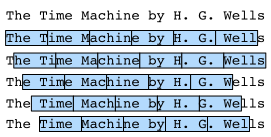
\includegraphics{images/ch3/timemachine-5gram.svg}
% 	\caption{ifferent offsets lead to different subsequences when splitting up text.}
% 	\label{fig:timemachine-5gram}
% \end{figure}

% In fact, any one of these offsets is fine. Hence, which one should we pick? In fact, all of them are equally good. But if we pick all offsets we end up with rather redundant data due to overlap, particularly if the sequences are long. Picking just a random set of initial positions is no good either since it does not guarantee uniform coverage of the array. For instance, if we pick $n$ elements at random out of a set of $n$ with random replacement, the probability for a particular element not being picked is $(1-1/n)^n \to e^{-1}$. This means that we cannot expect uniform coverage this way. Even randomly permuting a set of all offsets does not offer good guarantees. Instead we can use a simple trick to get both coverage and randomness: use a random offset, after which one uses the terms sequentially. This can be done both for random sampling and sequential partitioning.

% \paragraph{Random sampling}

% Randomly generates a minibatch from the data each time. In random sampling, each example is a sequence arbitrarily captured on the original sequence. The positions of two adjacent random mini-batches on the original sequence are not necessarily adjacent. The target is to predict the next character based on what we’ve seen so far, hence the labels are the original sequence, shifted by one character. Note that this is not recommended for latent variable models, since we do not have access to the hidden state prior to seeing the sequence. 

% \paragraph{Sequential partitioning}

% In addition to random sampling of the original sequence, we can also make the positions of two adjacent random mini-batches adjacent in the original sequence. Now, we can use a hidden state of the last time step of a mini-batch to initialize the hidden state of the next mini-batch, so that the output of the next mini-batch is also dependent on the input of the mini-batch, with this pattern continuing in subsequent mini-batches. This has two effects on the implementation of a recurrent neural network. On the one hand, when training the model, we only need to initialize the hidden state at the beginning of each epoch. On the other hand, when multiple adjacent mini-batches are concatenated by passing hidden states, the gradient calculation of the model parameters will depend on all the mini-batch sequences that are concatenated. In the same epoch as the number of iterations increases, the costs of gradient calculation rise. So that the model parameter gradient calculations only depend on the mini-batch sequence read by one iteration, we can separate the hidden state from the computational graph before reading the mini-batch (this can be done by detaching the graph).

% \subsubsection{One-hot Encoding}

% One-hot encoding vectors provide an easy way to express words as vectors in order to process them in a deep network. In a nutshell, we map each word to a different unit vector: assume that the number of different characters in the dictionary is N and each character has a one-to-one correspondence with a single value in the index of successive integers from 0 to N-1. If the index of a character is the integer i, then we create a vector $\mathbf{e}_i$ of all 0s with a length of N and set the element at position i to 1. This vector is the one-hot vector of the original character. The one-hot vectors with indices 0 and 2 are shown below (the length of the vector is equal to the dictionary size).


\subsection{Training Recurrent Networks: Backpropagation Through Time (BPTT)}

In this section we will delve a bit more deeply into the details of backpropagation for sequence models and why (and how) the math works.

Forward propagation in a recurrent neural network is relatively straightforward. Back-propagation through time is actually a specific application of back propagation in recurrent neural networks. It requires us to expand the recurrent neural network one time step at a time to obtain the dependencies between model variables and parameters. Then, based on the chain rule, we apply back propagation to compute and store gradients. Since sequences can be rather long this means that the dependency can be rather lengthy. E.g. for a sequence of 1000 characters the first symbol could potentially have significant influence on the symbol at position 1000. This is not really computationally feasible (it takes too long and requires too much memory) and it requires over 1000 matrix-vector products before we would arrive at that very elusive gradient. This is a process fraught with computational and statistical uncertainty. In the following we will address what happens and how to address this in practice.

\subsubsection{A Simplified Recurrent Network}

We start with a simplified model of how an RNN works. This model ignores details about the specifics of the hidden state and how it is being updated. These details are immaterial to the analysis and would only serve to clutter the notation and make it look more intimidating.

$$h_t = f(x_t, h_{t-1}, w) \text{ and } o_t = g(h_t, w)$$

Here $h_t$ denotes the hidden state, $x_t$ the input and $o_t$ the output. We have a chain of values $\{\ldots (h_{t-1}, x_{t-1}, o_{t-1}), (h_{t}, x_{t}, o_t), \ldots\}$ that depend on each other via recursive computation. The forward pass is fairly straightforward. All we need is to loop through the $(x_t, h_t, o_t)$ triples one step at a time. This is then evaluated by an objective function measuring the discrepancy between outputs $o_t$ and some desired target $y_t$

$$L(x,y, w) = \sum_{t=1}^T l(y_t, o_t)$$

For backpropagation matters are a bit more tricky. Let’s compute the gradients with regard to the parameters $w$ of the objective function $L$. We get that

$$
\begin{aligned}
\partial_{w} L & = \sum_{t=1}^T \partial_w l(y_t, o_t) \\
    & = \sum_{t=1}^T \partial_{o_t} l(y_t, o_t) \left[\partial_w g(h_t, w) + \partial_{h_t} g(h_t,w) \partial_w h_t\right]
\end{aligned}
$$

The first part of the derivative is easy to compute (this is after all the instantaneous loss gradient at time $t$). The second part is where things get tricky, since we need to compute the effect of the parameters on $h_t$. For each term we have the recursion:

$$
\begin{aligned}
    \partial_w h_t & = \partial_w f(x_t, h_{t-1}, w) + \partial_h f(x_t, h_{t-1}, w) \partial_w h_{t-1} \\
    & = \sum_{i=t}^1 \left[\prod_{j=t}^i \partial_h f(x_j, h_{j-1}, w) \right] \partial_w f(x_{i}, h_{i-1}, w)
\end{aligned}
$$

This chain can get very long whenever $t$ is large. While we can use the chain rule to compute $\partial_w h_t$ recursively, this might not be ideal. Let’s discuss a number of strategies for dealing with this problem:

\textbf{Compute the full sum}. This is very slow and gradients can blow up, since subtle changes in the initial conditions can potentially affect the outcome a lot. That is, we could see things similar to the butterfly effect where minimal changes in the initial conditions lead to disproportionate changes in the outcome. This is actually quite undesirable in terms of the model that we want to estimate. After all, we are looking for robust estimators that generalize well. Hence this strategy is almost never used in practice.

\textbf{Truncate the sum after $\tau$ steps}. This is what we have been discussing so far. This leads to an approximation of the true gradient, simply by terminating the sum above at $\partial_w h_{t-\tau}$. The approximation error is thus given by $\partial_h f(x_t, h_{t-1}, w) \partial_w h_{t-1}$ (multiplied by a product of gradients involving $\partial_h f$). In practice this works quite well. It is what is commonly referred to as truncated BPTT (backpropgation through time). One of the consequences of this is that the model focuses primarily on short-term influence rather than long-term consequences. This is actually desirable, since it biases the estimate towards simpler and more stable models.

\subsubsection{The Computational Graph}

In order to visualize the dependencies between model variables and parameters during computation in a recurrent neural network, we can draw a computational graph for the model, as shown below. For example, the computation of the hidden states of time step 3 $\mathbf{h}_3$ depends on the model parameters $\mathbf{W}_{hx}$ and $\mathbf{W}_{hh}$, the hidden state of the last time step $\mathbf{h}_2$, and the input of the current time step $\mathbf{x}_3.$

\begin{figure}[hpt]
	\centering
	\includesvg[scale=0.8]{images/ch3/rnn-bptt.svg}
	\caption{Computational dependencies for a recurrent neural network model with three time steps. Boxes represent variables (not shaded) or parameters (shaded) and circles represent operators.}
	\label{fig:rnn-bptt}
\end{figure}

\subsubsection{BPTT in Detail}

Now that we discussed the general principle let’s discuss BPTT in detail, distinguishing between different sets of weight matrices $(\mathbf{W}_{hx}, \mathbf{W}_{hh} and \mathbf{W}_{oh})$ in a simple linear latent variable model:

$$\mathbf{h}_t = \mathbf{W}_{hx} \mathbf{x}_t + \mathbf{W}_{hh} \mathbf{h}_{t-1} \text{ and }\mathbf{o}_t = \mathbf{W}_{oh} \mathbf{h}_t$$

We compute gradients $\partial L/\partial \mathbf{W}_{hx}$, $\partial L/\partial \mathbf{W}_{hh}$, and $\partial L/\partial \mathbf{W}_{oh}$ for $L(\mathbf{x}, \mathbf{y}, \mathbf{W}) = \sum_{t=1}^T l(\mathbf{o}_t, y_t)$. Taking the derivatives with respect to $W_{oh}$ is fairly straightforward and we obtain

$$\partial_{\mathbf{W}_{oh}} L = \sum_{t=1}^T \mathrm{prod}
\left(\partial_{\mathbf{o}_t} l(\mathbf{o}_t, y_t), \mathbf{h}_t\right)$$

The dependency on $\mathbf{W}_{hx}$ and $\mathbf{W}_{hh}$ is a bit more tricky since it involves a chain of derivatives. We begin with

$$
\begin{aligned}
\partial_{\mathbf{W}_{hh}} L & = \sum_{t=1}^T \mathrm{prod}
\left(\partial_{\mathbf{o}_t} l(\mathbf{o}_t, y_t), \mathbf{W}_{oh}, \partial_{\mathbf{W}_{hh}} \mathbf{h}_t\right) \\
\partial_{\mathbf{W}_{hx}} L & = \sum_{t=1}^T \mathrm{prod}
\left(\partial_{\mathbf{o}_t} l(\mathbf{o}_t, y_t), \mathbf{W}_{oh}, \partial_{\mathbf{W}_{hx}} \mathbf{h}_t\right)
\end{aligned}
$$

After all, hidden states depend on each other and on past inputs. The key quantity is how past hidden states affect future hidden states.

$$\partial_{\mathbf{h}_t} \mathbf{h}_{t+1} = \mathbf{W}_{hh}^\top \text{ and thus } \partial_{\mathbf{h}_t} \mathbf{h}_T = \left(\mathbf{W}_{hh}^\top\right)^{T-t}$$

Chaining terms together yields

$$
\begin{aligned}
\partial_{\mathbf{W}_{hh}} \mathbf{h}_t & = \sum_{j=1}^t \left(\mathbf{W}_{hh}^\top\right)^{t-j} \mathbf{h}_j \\
\partial_{\mathbf{W}_{hx}} \mathbf{h}_t & = \sum_{j=1}^t \left(\mathbf{W}_{hh}^\top\right)^{t-j} \mathbf{x}_j.
\end{aligned}
$$

A number of things follow from this potentially very intimidating expression. Firstly, it pays to store intermediate results, i.e. powers of $\mathbf{W}_{hh}$ as we work our way through the terms of the loss function $L$. Secondly, this simple linear example already exhibits some key problems of long sequence models: it involves potentially very large powers $\mathbf{W}_{hh}^j$. In it, eigenvalues smaller than 1 vanish for large $j$ and eigenvalues larger than 1 diverge. This is numerically unstable and gives undue importance to potentially irrelevant past detail. One way to address this is to truncate the sum at a computationally convenient size. Later on in this chapter we will see how more sophisticated sequence models such as LSTMs can alleviate this further. In code, this truncation is effected by detaching the gradient after a given number of steps.

\subsection{Gated Recurrent Units (GRU)}\label{subsec:gru}

In the previous section we discussed how gradients are calculated in a recurrent neural network. In particular we found that long products of matrices can lead to vanishing or divergent gradients. Let’s briefly think about what such gradient anomalies mean in practice:

We might encounter a situation where an early observation is highly significant for predicting all future observations. Consider the somewhat contrived case where the first observation contains a checksum and the goal is to discern whether the checksum is correct at the end of the sequence. In this case the influence of the first token is vital. We would like to have some mechanism for storing vital early information in a memory cell. Without such a mechanism we will have to assign a very large gradient to this observation, since it affects all subsequent observations.
We might encounter situations where some symbols carry no pertinent observation. For instance, when parsing a webpage there might be auxiliary HTML code that is irrelevant for the purpose of assessing the sentiment conveyed on the page. We would like to have some mechanism for skipping such symbols in the latent state representation.
We might encounter situations where there is a logical break between parts of a sequence. For instance there might be a transition between chapters in a book, a transition between a bear and a bull market for securities, etc.; In this case it would be nice to have a means of resetting our internal state representation.
A number of methods have been proposed to address this. One of the earliest is the Long Short Term Memory (LSTM) of \citep{Hochreiter1997}, which we will discuss in \cref{subsec:lstm}. The Gated Recurrent Unit (GRU) of \citet{Cho2014}, is a slightly more streamlined variant that often offers comparable performance and is significantly faster to compute. See also \citep{Chung2014} for more details. Due to its simplicity we start with the GRU.

\subsubsection{Gating the Hidden State}

The key distinction between regular RNNs and GRUs is that the latter support gating of the hidden state. This means that we have dedicated mechanisms for when the hidden state should be updated and also when it should be reset. These mechanisms are learned and they address the concerns listed above. For instance, if the first symbol is of great importance we will learn not to update the hidden state after the first observation. Likewise, we will learn to skip irrelevant temporary observations. Lastly, we will learn to reset the latent state whenever needed. We discuss this in detail below.

\paragraph{Reset Gates and Update Gates}

The first thing we need to introduce are reset and update gates. We engineer them to be vectors with entries in $(0,1)$ such that we can perform convex combinations, e.g.\ of a hidden state and an alternative. For instance, a reset variable would allow us to control how much of the previous state we might still want to remember. Likewise, an update variable would allow us to control how much of the new state is just a copy of the old state.

We begin by engineering gates to generate these variables. \cref{fig:gru_1} illustrates the inputs for both reset and update gates in a GRU, given the current time step input $\mathbf{X}_t$ and the hidden state of the previous time step $\mathbf{H}_{t-1}$. The output is given by a fully connected layer with a sigmoid as its activation function.

\begin{figure}[hpt]
	\centering
	\includesvg[scale=0.8]{images/ch3/gru_1.svg}
	\caption{Reset and update gate in a GRU.}
	\label{fig:gru_1}
\end{figure}

Here, we assume there are $h$ hidden units and, for a given time step $t$, the mini-batch input is $\mathbf{X}_t \in \mathbb{R}^{n \times d}$ (number of examples: $n$, number of inputs: $d$) and the hidden state of the last time step is $\mathbf{H}_{t-1} \in \mathbb{R}^{n \times h}$. Then, the reset gate $\mathbf{R}_t \in \mathbb{R}^{n \times h}$ and update gate $\mathbf{Z}_t \in \mathbb{R}^{n \times h}$ are computed as follows:

$$
\begin{aligned}
\mathbf{R}_t = \sigma(\mathbf{X}_t \mathbf{W}_{xr} + \mathbf{H}_{t-1} \mathbf{W}_{hr} + \mathbf{b}_r)\\
\mathbf{Z}_t = \sigma(\mathbf{X}_t \mathbf{W}_{xz} + \mathbf{H}_{t-1} \mathbf{W}_{hz} + \mathbf{b}_z)
\end{aligned}
$$

Here, $\mathbf{W}_{xr}, \mathbf{W}_{xz} \in \mathbb{R}^{d \times h}$ and $\mathbf{W}_{hr}, \mathbf{W}_{hz} \in \mathbb{R}^{h \times h}$ are weight parameters and $\mathbf{b}_r, \mathbf{b}_z \in \mathbb{R}^{1 \times h}$ are biases. We use a sigmoid function to transform values to the interval $(0,1)$.

\paragraph{Reset Gate in Action}

We begin by integrating the reset gate with a regular latent state updating mechanism. In a conventional deep RNN we would have an update of the form

$$\mathbf{H}_t = \tanh(\mathbf{X}_t \mathbf{W}_{xh} + \mathbf{H}_{t-1}\mathbf{W}_{hh} + \mathbf{b}_h)$$

This is essentially identical to the discussion of the previous section, albeit with a nonlinearity in the form of $\tanh$ to ensure that the values of the hidden state remain in the interval $(-1, 1)$.
If we want to be able to reduce the influence of previous states we can multiply $\mathbf{H}_{t-1}$ with $\mathbf{R}_t$ elementwise. Whenever the entries in $\mathbf{R}_t$ are close to $1$ we recover a conventional deep RNN. For all entries of $\mathbf{R}_t$ that are close to $0$ the hidden state is the result of an MLP with $\mathbf{X}_t$ as input. Any pre-existing hidden state is thus 'reset' to defaults. This leads to the following candidate for a new hidden state (it is a \textit{candidate} since we still need to incorporate the action of the update gate).

$$\tilde{\mathbf{H}}_t = \tanh(\mathbf{X}_t \mathbf{W}_{xh} + \left(\mathbf{R}_t \odot \mathbf{H}_{t-1}\right) \mathbf{W}_{hh} + \mathbf{b}_h)$$

\cref{fig:gru_2} illustrates the computational flow after applying the reset gate. The symbol $\odot$ indicates pointwise multiplication between tensors.

\begin{figure}[hpt]
	\centering
	\includesvg[scale=0.8]{images/ch3/gru_2.svg}
	\caption{Candidate hidden state computation in a GRU. The multiplication is carried out elementwise.}
	\label{fig:gru_2}
\end{figure}

\paragraph{Update Gate in Action}

Next we need to incorporate the effect of the update gate. This determines the extent to which the new state $\mathbf{H}_t$ is just the old state $\mathbf{H}_{t-1}$ and by how much the new candidate state $\tilde{\mathbf{H}}_t$ is used. The gating variable $\mathbf{Z}_t$ can be used for this purpose, simply by taking elementwise convex combinations between both candidates. This leads to the final update equation for the GRU.

$$\mathbf{H}_t = \mathbf{Z}_t \odot \mathbf{H}_{t-1}  + (1 - \mathbf{Z}_t) \odot \tilde{\mathbf{H}}_t$$

\begin{figure}[hpt]
	\centering
	\includesvg[scale=0.8]{images/ch3/gru_3.svg}
	\caption{Hidden state computation in a GRU. As before, the multiplication is carried out elementwise.}
	\label{fig:gru_3}
\end{figure}

Whenever the update gate is close to $1$ we simply retain the old state. In this case the information from $\mathbf{X}_t$ is essentially ignored, effectively skipping time step $t$ in the dependency chain. Whenever it is close to $1$ the new latent state $\mathbf{H}_t$ approaches the candidate latent state $\tilde{\mathbf{H}}_t$. These designs can help cope with the vanishing gradient problem in RNNs and better capture dependencies for time series with large time step distances. In summary GRUs have the following two distinguishing features:

\begin{itemize}
    \item Reset gates help capture short-term dependencies in time series.
    \item Update gates help capture long-term dependencies in time series.
\end{itemize}

\subsection{Long Short Term Memory (LSTM)}\label{subsec:lstm}

The challenge to address long-term information preservation and short-term input skipping in latent variable models has existed for a long time. One of the earliest approaches to address this was the LSTM by Hochreiter and Schmidhuber, 1997. It shares many of the properties of the Gated Recurrent Unit (GRU) and predates it by almost two decades. Its design is slightly more complex.

Arguably it is inspired by logic gates of a computer. To control a memory cell we need a number of gates. One gate is needed to read out the entries from the cell (as opposed to reading any other cell). We will refer to this as the \textit{output} gate. A second gate is needed to decide when to read data into the cell. We refer to this as the \textit{input} gate. Lastly, we need a mechanism to reset the contents of the cell, governed by a \textit{forget} gate. The motivation for such a design is the same as before, namely to be able to decide when to remember and when to ignore inputs into the latent state via a dedicated mechanism. Let’s see how this works in practice.

\subsubsection{Gated Memory Cells}

Three gates are introduced in LSTMs: the input gate, the forget gate, and the output gate. In addition to that we introduce memory cells that take the same shape as the hidden state. Strictly speaking this is just a fancy version of a hidden state, custom engineered to record additional information.

\paragraph{Input Gates, Forget Gates and Output Gates}

Just like with GRUs, the data feeding into the LSTM gates is the input at the current time step $\mathbf{X}_t$ and the hidden state of the previous time step $\mathbf{H}_{t-1}$. These inputs are processed by a fully connected layer and a sigmoid activation function to compute the values of input, forget and output gates. As a result, the three gate elements all have a value range of $[0,1]$.

\begin{figure}[hpt]
	\centering
	\includesvg[scale=0.8]{images/ch3/lstm_0.svg}
	\caption{Calculation of input, forget, and output gates in an LSTM.}
	\label{fig:lstm_0}
\end{figure}

We assume there are $h$ hidden units and that the minibatch is of size $n$. Thus
the input is $\mathbf{X}_t \in \mathbb{R}^{n \times d}$ (number of examples:
$n$, number of inputs: $d$) and the hidden state of the last time step is $\mathbf{H}_{t-1} \in \mathbb{R}^{n \times h}$. Correspondingly the gates are defined as follows: the input gate is $\mathbf{I}_t \in \mathbb{R}^{n \times h}$, the forget gate is $\mathbf{F}_t \in \mathbb{R}^{n \times h}$, and the output gate is $\mathbf{O}_t \in \mathbb{R}^{n \times h}$. They are calculated as follows:

$$
\begin{aligned}
\mathbf{I}_t &= \sigma(\mathbf{X}_t \mathbf{W}_{xi} + \mathbf{H}_{t-1} \mathbf{W}_{hi} + \mathbf{b}_i),\\
\mathbf{F}_t &= \sigma(\mathbf{X}_t \mathbf{W}_{xf} + \mathbf{H}_{t-1} \mathbf{W}_{hf} + \mathbf{b}_f),\\
\mathbf{O}_t &= \sigma(\mathbf{X}_t \mathbf{W}_{xo} + \mathbf{H}_{t-1} \mathbf{W}_{ho} + \mathbf{b}_o),
\end{aligned}
$$

$\mathbf{W}_{xi}, \mathbf{W}_{xf}, \mathbf{W}_{xo} \in \mathbb{R}^{d \times h}$ and $\mathbf{W}_{hi}, \mathbf{W}_{hf}, \mathbf{W}_{ho} \in \mathbb{R}^{h \times h}$ are weight parameters and $\mathbf{b}_i, \mathbf{b}_f, \mathbf{b}_o \in \mathbb{R}^{1 \times h}$ are bias parameters.

\paragraph{Candidate Memory Cell}

Next we design a memory cell. Since we haven't specified the action of the various gates yet, we first introduce a \textit{candidate} memory cell $\tilde{\mathbf{C}}_t \in \mathbb{R}^{n \times h}$. Its computation is similar to the three gates described above, but using a $\tanh$ function with a value range for $[-1, 1]$ as activation function. This leads to the following equation at time step $t$.

$$\tilde{\mathbf{C}}_t = \text{tanh}(\mathbf{X}_t \mathbf{W}_{xc} + \mathbf{H}_{t-1} \mathbf{W}_{hc} + \mathbf{b}_c)$$

Here $\mathbf{W}_{xc} \in \mathbb{R}^{d \times h}$ and $\mathbf{W}_{hc} \in \mathbb{R}^{h \times h}$ are weights and $\mathbf{b}_c \in \mathbb{R}^{1 \times h}$ is a bias.

\begin{figure}[hpt]
	\centering
	\includesvg[scale=0.8]{images/ch3/lstm_1.svg}
	\caption{Computation of candidate memory cells in LSTM.}
	\label{fig:lstm_1}
\end{figure}


\paragraph{Memory Cell}

In GRUs we had a single mechanism to govern input and forgetting. Here we have two parameters, $\mathbf{I}_t$ which governs how much we take new data into account via $\tilde{\mathbf{C}}_t$ and the forget parameter $\mathbf{F}_t$ which addresses how much we of the old memory cell content $\mathbf{C}_{t-1} \in \mathbb{R}^{n \times h}$ we retain. Using the same pointwise multiplication trick as before we arrive at the following update equation.

$$\mathbf{C}_t = \mathbf{F}_t \odot \mathbf{C}_{t-1} + \mathbf{I}_t \odot \tilde{\mathbf{C}}_t.$$

If the forget gate is always approximately 1 and the input gate is always approximately 0, the past memory cells will be saved over time and passed to the current time step. This design was introduced to alleviate the vanishing gradient problem and to better capture dependencies for time series with long range dependencies. We thus arrive at the following flow diagram.

\begin{figure}[hpt]
	\centering
	\includesvg[scale=0.8]{images/ch3/lstm_2.svg}
	\caption{Computation of memory cells in an LSTM. Here, the multiplication is carried out element-wise.}
	\label{fig:lstm_2}
\end{figure}

\paragraph{Hidden States}

Lastly we need to define how to compute the hidden state $\mathbf{H}_t \in \mathbb{R}^{n \times h}$. This is where the output gate comes into play. In the LSTM it is simply a gated version of the $\tanh$ of the memory cell. This ensures that the values of $\mathbf{H}_t$ are always in the interval $[-1, 1]$. Whenever the output gate is $1$ we effectively pass all memory information through to the predictor whereas for output $0$ we retain all information only within the memory cell and perform no further processing. \cref{fig:lstm_3} has a graphical illustration of the data flow.

$$\mathbf{H}_t = \mathbf{O}_t \odot \tanh(\mathbf{C}_t).$$

\begin{figure}[hpt]
	\centering
	\includesvg[scale=0.8]{images/ch3/lstm_3.svg}
	\caption{Computation of the hidden state. Multiplication is element-wise.}
	\label{fig:lstm_3}
\end{figure}

% \subsection{Deep Recurrent Neural Networks}

% Up to now, we only discussed recurrent neural networks with a single unidirectional hidden layer. In it the specific functional form of how latent variables and observations interact was rather arbitrary. This isn't a big problem as long as we have enough flexibility to model different types of interactions. With a single layer, however, this can be quite challenging. In the case of the perceptron we fixed this problem by adding more layers. Within RNNs this is a bit more tricky, since we first need to decide how and where to add extra nonlinearity. Our discussion below focuses primarily on LSTMs but it applies to other sequence models, too.

% \begin{itemize}
%     \item We could add extra nonlinearity to the gating mechansims. That is, instead of using a single perceptron we could use multiple layers. This leaves the \textit{mechanism} of the LSTM unchanged. Instead it makes it more sophisticated. This would make sense if we were led to believe that the LSTM mechanism describes some form of universal truth of how latent variable autoregressive models work.
%     \item We could stack multiple layers of LSTMs on top of each other. This results in a mechanism that is more flexible, due to the combination of several simple layers. In particular, data might be relevant at different levels of the stack. For instance, we might want to keep high-level data about financial market conditions (bear or bull market) available at a high level, whereas at a lower level we only record shorter-term temporal dynamics.
% \end{itemize}

% Beyond all this abstract discussion it is probably easiest to understand the family of models we are interested in by reviewing the diagram below. It describes a deep recurrent neural network with $L$ hidden layers. Each hidden state is continuously passed to the next time step of the current layer and the next layer of the current time step.

% \begin{figure}[hpt]
% 	\centering
% 	\includesvg[scale=0.8]{images/ch3/deep-rnn.svg}
% 	\caption{Architecture of a deep recurrent neural network.}
% 	\label{fig:deep-rnn}
% \end{figure}

% \subsubsection{Functional Dependencies}

% At time step $t$ we assume that we have a minibatch $\mathbf{X}_t \in \mathbb{R}^{n \times d}$ (number of examples: $n$, number of inputs: $d$). The hidden state of hidden layer $\ell$ ($\ell=1,\ldots,T$) is $\mathbf{H}_t^{(\ell)}  \in \mathbb{R}^{n \times h}$ (number of hidden units: $h$), the output layer variable is $\mathbf{O}_t \in \mathbb{R}^{n \times q}$ (number of outputs: $q$) and a hidden layer activation function $f_l$ for layer $l$. We compute the hidden state of layer $1$ as before, using $\mathbf{X}_t$ as input. For all subsequent layers the hidden state of the previous layer is used in its place.

% $$\begin{aligned}
% \mathbf{H}_t^{(1)} & = f_1\left(\mathbf{X}_t, \mathbf{H}_{t-1}^{(1)}\right) \\
% \mathbf{H}_t^{(l)} & = f_l\left(\mathbf{H}_t^{(l-1)}, \mathbf{H}_{t-1}^{(l)}\right)
% \end{aligned}$$

% Finally, the output of the output layer is only based on the hidden state of hidden layer $L$. We use the output function $g$ to address this:

% $$\mathbf{O}_t = g \left(\mathbf{H}_t^{(L)}\right)$$

% Just as with multilayer perceptrons, the number of hidden layers $L$ and number of hidden units $h$ are hyper parameters. In particular, we can pick a regular RNN, a GRU or an LSTM to implement the model.

% \subsection{Bidirectional Recurrent Neural Networks}

% So far we assumed that our goal is to model the next word given what we've seen so far, e.g. in the context of a time series or in the context of a language model. While this is a typical scenario, it is not the only one we might encounter. To illustrate the issue, consider the following three tasks of filling in the blanks in a text:

% \begin{verbatim}
% I am _____
% I am _____ very hungry.
% I am _____ very hungry, I could eat half a pig.    
% \end{verbatim}

% Depending on the amount of information available we might fill the blanks with very different words such as 'happy', 'not', and 'very'. Clearly the end of the phrase (if available) conveys significant information about which word to pick. A sequence model that is incapable of taking advantage of this will perform poorly on related tasks. For instance, to do well in named entity recognition (e.g. to recognize whether 'Green' refers to 'Mr. Green' or to the color) longer-range context is equally vital. To get some inspiration for addressing the problem let's take a detour to graphical models.

% \subsubsection{Dynamic Programming}

% This section serves to illustrate the problem. The specific technical details do not matter for understanding the deep learning counterpart but they help in motivating why one might use deep learning and why one might pick specific architectures.

% If we want to solve the problem using graphical models we could for instance design a latent variable model as follows: we assume that there exists some latent variable $h_t$ which governs the emissions $x_t$ that we observe via $p(x_t|h_t)$. Moreover, the transitions $h_t \to h_{t+1}$ are given by some state transition probability $p(h_t|h_{t-1})$. The graphical model then looks as follows:

% \begin{figure}[hpt]
% 	\centering
% 	\includesvg[scale=0.8]{images/ch3/hmm.svg}
% 	\caption{Hidden Markov Model.}
% 	\label{fig:hmm}
% \end{figure}

% For a sequence of $T$ observations we have thus the following joint probability distribution over observed and hidden states:

% $$p(x,h) = p(h_1) p(x_1|h_1) \prod_{i=2}^T p(h_t|h_{t-1}) p(x_t|h_t)$$

% Now assume that we observe all $x_i$ with the exception of some $x_j$ and it is our goal to compute $p(x_j|x^{-j})$. To accomplish this we need to sum over all possible choices of $h = (h_1, \ldots, h_T)$. In case $h_i$ can take on $k$ distinct values this means that we need to sum over $k^T$ terms - mission impossible! Fortunately there's an elegant solution for this: \textbf{dynamic programming}. To see how it works consider summing over the first two hidden variable $h_1$ and $h_2$. This yields:

% $$\begin{aligned}
%     p(x) & = \sum_h p(h_1) p(x_1|h_1) \prod_{i=2}^T p(h_t|h_{t-1}) p(x_t|h_t) \\
%     & = \sum_{h_2, \ldots h_T} \underbrace{\left[\sum_{h_1} p(h_1) p(x_1|h_1) p(h_2|h_1)\right]}_{=: \pi_2(h_2)}
%     p(x_2|h_2) \prod_{i=2}^T p(h_t|h_{t-1}) p(x_t|h_t) \\
%     & = \sum_{h_3, \ldots h_T} \underbrace{\left[\sum_{h_2} \pi_2(h_2) p(x_2|h_2) p(h_3|h_2)\right]}_{=: \pi_3(h_3)}
%     p(x_3|h_3) \prod_{i=3}^T p(h_t|h_{t-1}) p(x_t|h_t)
% \end{aligned}$$

% In general we have the \textit{forward} recursion

% $$\pi_{t+1}(h_{t+1}) = \sum_{h_t} \pi_t(h_t) p(x_t|h_t) p(h_{t+1}|h_1)$$

% The recursion is initialized as $\pi_1(h_1) = p(h_1)$. In abstract terms this can be written as $\pi_{t+1} = f(\pi_t, x_t)$, where $f$ is some learned function. This looks very much like the update equation in the hidden variable models we discussed so far in the context of RNNs. Entirely analogously to the forward recursion we can also start a backwards recursion. This yields:

% $$\begin{aligned}
%     p(x) & = \sum_h \prod_{i=1}^{T-1} p(h_t|h_{t-1}) p(x_t|h_t) \cdot p(h_T|h_{T-1}) p(x_T|h_T) \\
%     & = \sum_{h_1, \ldots h_{T-1}} \prod_{i=1}^{T-1} p(h_t|h_{t-1}) p(x_t|h_t) \cdot
%     \underbrace{\left[\sum_{h_T} p(h_T|h_{T-1}) p(x_T|h_T)\right]}_{=: \rho_{T-1}(h_{T-1})} \\
%     & = \sum_{h_1, \ldots h_{T-2}} \prod_{i=1}^{T-2} p(h_t|h_{t-1}) p(x_t|h_t) \cdot
%     \underbrace{\left[\sum_{h_{T-1}} p(h_{T-1}|h_{T-2}) p(x_{T-1}|h_{T-1})\right]}_{=: \rho_{T-2}(h_{T-2})}
% \end{aligned}$$

% We can thus write the \textit{backward} recursion as

% $$\rho_{t-1}(h_{t-1})= \sum_{h_{t}} p(h_{t}|h_{t-1}) p(x_{t}|h_{t})$$

% with initialization $\rho_T(h_T) = 1$. These two recursions allow us to sum over $T$ variables in $O(kT)$ (linear) time over all values of $(h_1, \ldots h_T)$ rather than in exponential time. This is one of the great benefits of probabilistic inference with graphical models. It is a very special instance of the [Generalized Distributive Law](https://authors.library.caltech.edu/1541/1/AJIieeetit00.pdf) proposed in 2000 by Aji and McEliece. Combining both forward and backward pass we are able to compute

% $$p(x_j|x_{-j}) \propto \sum_{h_j} \pi_j(h_j) \rho_j(h_j) p(x_j|h_j).$$

% Note that in abstract terms the backward recursion can be written as $\rho_{t-1} = g(\rho_t, x_t)$, where $g$ is some learned function. Again, this looks very much like an update equation, just running backwards unlike what we've seen so far in RNNs. And, indeed, HMMs benefit from knowing future data when it is available. Signal processing scientists distinguish between the two cases of knowing and not knowing future observations as filtering vs. smoothing.

% \subsubsection{Bidirectional Model}

% If we want to have a mechanism in RNNs that offers comparable look-ahead ability as in HMMs we need to modify the recurrent net design we’ve seen so far. Fortunately this is easy (conceptually). Instead of running an RNN only in forward mode starting from the first symbol we start another one from the last symbol running back to front. Bidirectional recurrent neural networks add a hidden layer that passes information in a backward direction to more flexibly process such information. The figure below illustrates the architecture of a bidirectional recurrent neural network with a single hidden layer.

% \begin{figure}[hpt]
% 	\centering
% 	\includesvg{images/ch3/birnn.svg}
% 	\caption{Architecture of a bidirectional recurrent neural network.}
% 	\label{fig:birnn}
% \end{figure}

% In fact, this is not too dissimilar to the forward and backward recurrences we encountered above. The main distinction is that in the previous case these equations had a specific statistical meaning. Now they’re devoid of such easily accessible interpretation and we can just treat them as generic functions. This transition epitomizes many of the principles guiding the design of modern deep networks - use the type of functional dependencies common to classical statistical models and use them in a generic form.

% \paragraph{Definition}

% Bidirectional RNNs were introduced by \citet{Schuster1997}. For a detailed discussion of the various architectures see also the paper by \citet{Graves2005}. Let's look at the specifics of such a network. For a given time step $t$, the mini-batch input is $\mathbf{X}_t \in \mathbb{R}^{n \times d}$ (number of examples: $n$, number of inputs: $d$) and the hidden layer activation function is $\phi$. In the bidirectional architecture:
% We assume that the forward and backward hidden states for this time step are $\overrightarrow{\mathbf{H}}_t  \in \mathbb{R}^{n \times h}$ and $\overleftarrow{\mathbf{H}}_t  \in \mathbb{R}^{n \times h}$ respectively. Here $h$ indicates the number of hidden units. We compute the forward and backward hidden state updates as follows:

% $$
% \begin{aligned}
% \overrightarrow{\mathbf{H}}_t &= \phi(\mathbf{X}_t \mathbf{W}_{xh}^{(f)} + \overrightarrow{\mathbf{H}}_{t-1} \mathbf{W}_{hh}^{(f)}  + \mathbf{b}_h^{(f)}),\\
% \overleftarrow{\mathbf{H}}_t &= \phi(\mathbf{X}_t \mathbf{W}_{xh}^{(b)} + \overleftarrow{\mathbf{H}}_{t+1} \mathbf{W}_{hh}^{(b)}  + \mathbf{b}_h^{(b)}),
% \end{aligned}
% $$

% Here, the weight parameters $\mathbf{W}_{xh}^{(f)} \in \mathbb{R}^{d \times h}, \mathbf{W}_{hh}^{(f)} \in \mathbb{R}^{h \times h}, \mathbf{W}_{xh}^{(b)} \in \mathbb{R}^{d \times h}, and \mathbf{W}_{hh}^{(b)} \in \mathbb{R}^{h \times h}$ and bias parameters $\mathbf{b}_h^{(f)} \in \mathbb{R}^{1 \times h} and \mathbf{b}_h^{(b)} \in \mathbb{R}^{1 \times h}$ are all model parameters.

% Then we concatenate the forward and backward hidden states $\overrightarrow{\mathbf{H}}_t$ and $\overleftarrow{\mathbf{H}}_t$ to obtain the hidden state $\mathbf{H}_t \in \mathbb{R}^{n \times 2h}$ and input it to the output layer. In deep bidirectional RNNs the information is passed on as input to the next bidirectional layer. Lastly, the output layer computes the output $\mathbf{O}_t \in \mathbb{R}^{n \times q}$ (number of outputs: $q$):

% $$\mathbf{O}_t = \mathbf{H}_t \mathbf{W}_{hq} + \mathbf{b}_q,$$

% Here, the weight parameter $\mathbf{W}_{hq} \in \mathbb{R}^{2h \times q}$ and bias parameter $\mathbf{b}_q \in \mathbb{R}^{1 \times q}$ are the model parameters of the output layer. The two directions can have different numbers of hidden units.

% \paragraph{Computational Cost and Applications}

% One of the key features of a bidirectional RNN is that information from both ends of the sequence is used to estimate the output. That is, we use information from future and past observations to predict the current one (a smoothing scenario). In the case of language models this isn't quite what we want. After all, we don't have the luxury of knowing the next to next symbol when predicting the next one. Hence, if we were to use a bidirectional RNN naively we wouldn't get very good accuracy: during training we have past and future data to estimate the present. During test time we only have past data and thus poor accuracy (we will illustrate this in an experiment below).

% To add insult to injury bidirectional RNNs are also exceedingly slow. The main reason for this is that they require both a forward and a backward pass and that the backward pass is dependent on the outcomes of the forward pass. Hence gradients will have a very long dependency chain.

% In practice bidirectional layers are used very sparingly and only for a narrow set of applications, such as filling in missing words, annotating tokens (e.g. for named entity recognition), or encoding sequences wholesale as a step in a sequence processing pipeline (e.g. for machine translation). In short, handle with care!

\section{The Encoder-Decoder architecture}\label{sec:encoder-decoder}

\subsection{From feature engineering to feature learning}

Machine learning algorithms take features as inputs and produce some output. How we represent features makes a huge difference on the performance of the learning algorithms.  Traditionally, approaches to machine learning require a strong \textbf{feature engineering} approach, meaning that the designer has to carefully choose features and their representation before feeding them into the algorithm. When facing complex problems like computer vision, this approach came up with sophisticated representations, such as HOG (Histogram of Oriented Gradients) for representing image features.

Due to such representations, there is a difference to be made between the \textit{raw inputs}, and the features which are input to the model. For example, in face recognition, the pixels of a picture are the raw input, while the HOG features of the image can be the actual input to the model.

Someone came up with the idea that we can use an algorithm to learn the feature representation itself, aptly called \textbf{feature learning}. Deep learning uses a neural network model to achieve this task. In point of fact, feature learning is accomplished by the first layers of a neural network, which map raw inputs to efficient feature representations. The last layers (typically fully connected layers) mix and match and combine these features to produce an output.

\subsection{The encoder-decoder architecture}

The \textbf{encoder-decoder architecture} explicitly aims to leverage this ability of neural networks to learn efficient representations. It is a neural network design pattern that consists of two main components, the \textit{encoder} and the \textit{decoder}.  The \textbf{encoder} maps raw inputs to feature representations, and these representations are then passed to the \textbf{decoder}, which has to produce an output. This is commonly referred to as the encoder-decoder framework, and its general architecture is shown in \cref{fig:encoder-decoder}

\begin{figure}[hpt]
	\centering
	\includesvg{images/ch3/encoder-decoder.svg}
	\caption{The encoder-decoder architecture.}
	\label{fig:encoder-decoder}
\end{figure}

Theoretically, encoder and decoder parts can be used independently of each other. For instance, an encoder RNN can be used to encode the features of an incoming email as a \textit{features vector}, which is then used as input to a Fully-Connected Layer (FCL) to predict whether the email is spam or not. However, neural encoder and decoders are often used in a tightly coupled manner, meaning that the system is trained as a whole. This approach, known as \textbf{end-to-end}, is been increasingly used due to a combination of good performance and less engineering effort.

The encoder-decoder architecture is enormously popular in the fields of computer vision and natural language processing, and may adopt very different forms. In some cases, the same type of network is used for both the encoder and the encoder.

For example, \cref{fig:cnn-cnn} depicts an example of a pure convolutional encoder-decoder architecture (there is no fully connected layer). This model is used to perform semantic segmentation of an image. The left half of the network (the encoder) maps raw image pixels to a rich representation consisting of feature vectors. The right half of the network (the decoder) takes these features and upsamples them to produce a sparse feature map which is fed to a soft-max for pixel-wise classification.

\begin{figure}[hpt]
	\centering
	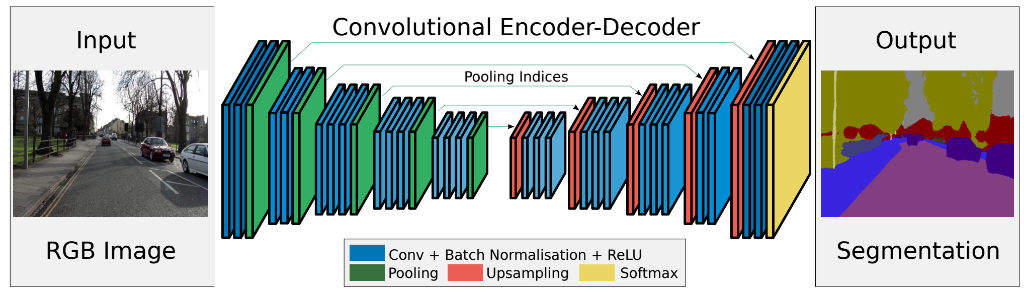
\includegraphics[scale=0.45]{images/ch3/cnn-cnn.png}
	\caption{Convolutional encoder-decoder for image segmentation in the SeqNet architecture \citep{Badrinarayanan2017}}
	\label{fig:cnn-cnn}
\end{figure}

Encoder-decoder networks based on RNN are very common in problems requiring \textit{sequence-to-sequence (seq2seq)} modelling, such as translation, summarising and question-answering. For example, \cref{fig:rnn-rnn} shows an example of a model used to generate automatic responses to incoming emails. The left half of the network encodes the email into a feature vector, and the right half of the network decodes the feature vector to produce word predictions. 

\begin{figure}[hpt]
	\centering
	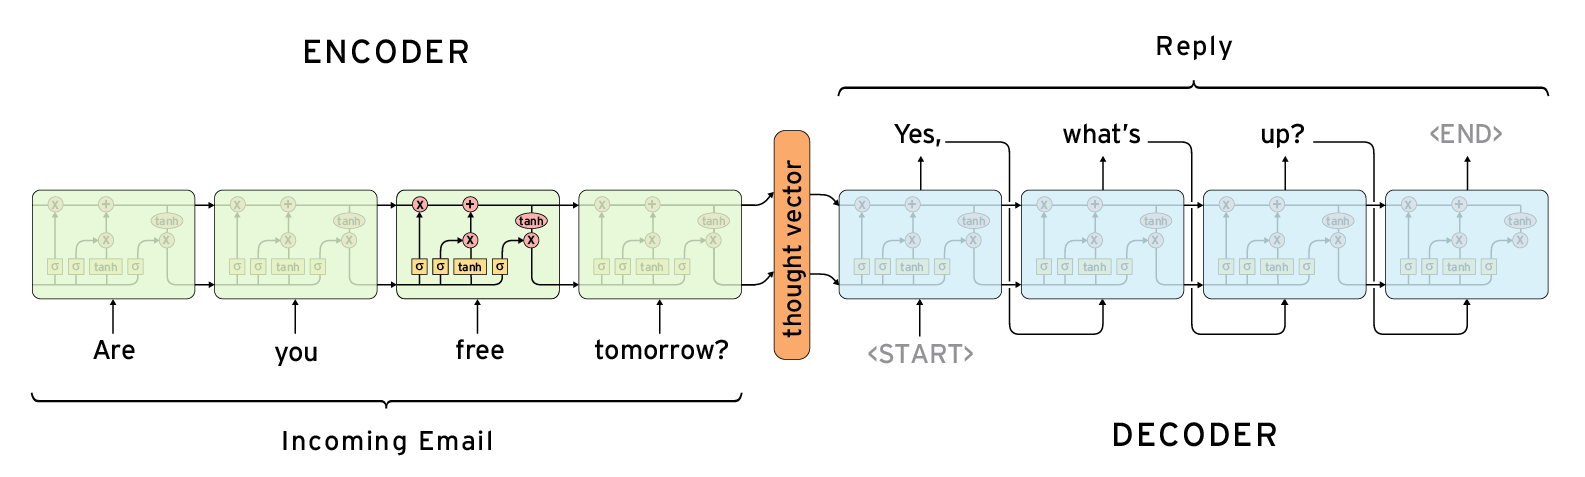
\includegraphics[scale=0.3]{images/ch3/rnn-rnn.png}
	\caption{Recurrent encoder-decoder for automated email answering. The model is given input a sentence and produces a response in the same language. Source: \href{https://ai.googleblog.com/2015/11/computer-respond-to-this-email.html}{Google AI Blog}}
	\label{fig:rnn-rnn}
\end{figure}

However, in general, an encoder-decoder network may hybridate different types of network. A common pattern is the CNN-RNN architecture, which uses a CNN as encoder and an RNN as decoder. This is a class of models that is both spatially and temporally deep, and has the flexibility to be applied to a variety of multimodal tasks involving visual inputs and sequential outputs. Some examples of tasks where this architecture is used include:

\begin{itemize}
    \item Visual time series forecasting: Predicting the evolution of series, such as stock prices or energy load.
    \item Activity recognition: Generating a textual description of an activity demonstrated in a sequence of images.
    \item Image captioning: Generating a textual description of a single image.
    \item Video description: Generating a textual description of a sequence of images.
\end{itemize}

This architecture was originally referred to as a Long-term Recurrent Convolutional Network (LRCN) \citep{Donahue2015}, since typically it uses LSTM for the recurrent part. For example, \cref{fig:cnn-rnn} depicts the Neural Image Captioner developed by Google \citep{Vinyals2015}, which uses  a Batch Normalization version of their Inception CNN for the encoder, and an LSTM network for the decoder. The model works as follows: first, the CNN process an image and extracts visual features, which are then passed as input to the LSTM. The LSTM takes a word, the context from previous time steps, and defines a probability distribution over the next word in the sentence. The LSTM is conditioned on the image information at the first time step. The generative process is started with a special "<start>" token, and ends when a special "<end>" token is generated.

\begin{figure}[hpt]
	\centering
	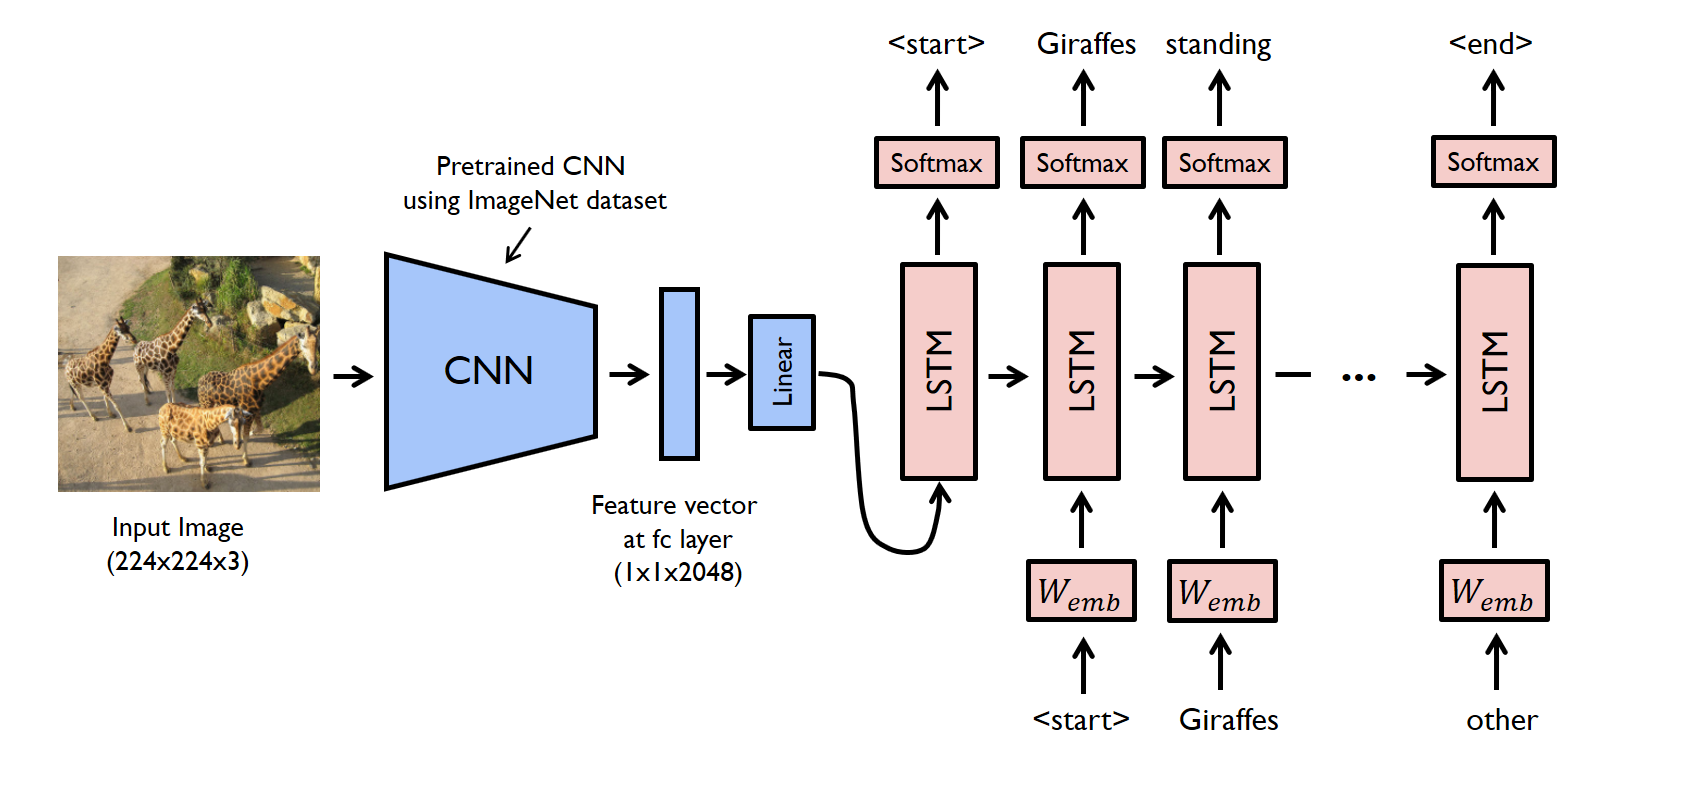
\includegraphics[scale=0.3]{images/ch3/cnn-rnn.png}
	\caption{Encoder-decoder combining CNN and LSTM for image captionign. Source:  \href{https://github.com/yunjey/pytorch-tutorial/tree/master/tutorials/03-advanced/image_captioning}{Yunjey Choi's implementation} of the Show and Tell model \citep{Vinyals2015}.}
	\label{fig:cnn-rnn}
\end{figure}

A key of this architecture is the use of a CNN that is pre-trained on a challenging image classification task, which is re-purposed as a feature extractor for the caption generating problem (this is called \textit{transfer learning}). Typically, a CNN trained on the ImageNet dataset is used for this purpose.

For the decoder, most systems proposed so far use LSTM units, since they are more powerful than other types of recurrent units, although lately, GRU units have also emerged as a viable alternative with similar capabilities bu reduced cost.

\subsection{Sequence to Sequence modelling}\label{subsec:seq2seq}

\subsubsection{Architecture of seq2seq model}

The sequence to sequence (seq2seq) model is based on the encoder-decoder architecture to generate a sequence output for a sequence input. Both the encoder and the decoder use recurrent neural networks to handle sequence inputs. The hidden state of the encoder is used directly to initialize the decoder hidden state to pass information from the encoder to the decoder.

\begin{figure}[hpt]
	\centering
	\includesvg{images/ch3/seq2seq.svg}
	\caption{The sequence to sequence model architecture.}
	\label{fig:seq2seq}
\end{figure}

The layers in the encoder and the decoder are illustrated in the following figure.

\begin{figure}[hpt]
	\centering
	\includesvg{images/ch3/seq2seq-details.svg}
	\caption{Layers in seq2seq model.}
	\label{fig:seq2seq_details}
\end{figure}

\subsubsubsection{The seq2seq encoder}

In the encoder, we use the word embedding layer to obtain a feature index from the word index of the input language and then input it into a multi-level recurrent layer, typicall made of gated recurrent units such as LSTM or GRU. The input for the encoder is a batch of sequences, which is 2-D tensor with shape (batch size, sequence length). The output consists of both the outputs of the recurrent units and the hidden states (and memory cells of the last time step if using LSTM).

The output shape returned by the encoder after performing forward calculation on the input is (number of time steps, batch size, number of hidden units). The shape of the multi-layer hidden state of the gated recurrent unit in the final time step is (number of hidden layers, batch size, number of hidden units). If GRU is used used the \textit{state}  contains only one element, which is the hidden state. If LSTM is used, the \textit{state} list will also contain another element, which is the memory cell.

\subsubsubsection{The seq2seq decoder}

We directly use the hidden state of the encoder in the final time step as the initial hidden state of the decoder. This requires that the encoder and decoder RNNs have the same numbers of layers and hidden units.

The forward calculation of the decoder is similar to the encoder's. The only difference is the addition of a dense layer with the hidden size to be the vocabulary size to output the predicted confidence score for each word.

\subsubsection{Training}

For each time step, the decoder outputs a vocabulary size confident score vector to predict words. Similar to language modeling, we can apply \textit{softmax} to obtain the probabilities and then use cross entropy loss to calculate the loss. 

But note that we padded the target sentences to make them have the same length. We would not like to compute the loss on the padding symbols. To solve that, a masked version of the loss function is used.

During training, if the target sequence has length $n$, we feed the first $n-1$ tokens into the decoder as inputs, and the last $n-1$ tokens are used as ground truth label. This is called \textit{Teacher Forcing}, and is depicted in \cref{fig:seq2seq}.

\subsubsection{Prediction}

In \cref{subsec:seq2seq}  we discussed how to train an encoder-decoder with input and output sequences that are both of variable length. In this section, we are going to introduce how to use the encoder-decoder to predict sequences of variable length.

\begin{figure}[hpt]
	\centering
	\includesvg{images/ch3/seq2seq_predict.svg}
	\caption{Sequence to sequence model predicting with greedy search.}
	\label{fig:seq2seq_predict}
\end{figure}

In general, prediction is done by feeding the same "<bos>" token to the decoder as training at time step 0. But the input token for a later time step is the predicted token from the previous time step, instead of the ground truth token used during training, as shown in \cref{fig:seq2seq_predict}.

Various approaches exist to predict the next token. For example, in greedy search, the token with the highest score at each time step is chosen and used to predict the next token. However, there are more sophisticated approaches, introduce below. 

\paragraph{Notation}

As in the previous section, when preparing to train the data set, we normally attach a special symbol "<eos>" after each sentence to indicate the termination of the sequence. We will continue to use this mathematical symbol in the discussion below. For ease of discussion, we assume that the output of the decoder is a sequence of text. Let the size of output text dictionary $\mathcal{Y}$ (contains special symbol "<eos>") be $\left|\mathcal{Y}\right|$, and the maximum length of the output sequence be $T'$. There are a total $\mathcal{O}(\left|\mathcal{Y}\right|^{T'})$ types of possible output sequences. All the subsequences after the special symbol "<eos>" in these output sequences will be discarded.


\subsubsubsection{Greedy Search}

First, we will take a look at a simple solution: greedy search. For any time step $t'$ of the output sequence, we are going to search for the word with the highest conditional probability from $|\mathcal{Y}|$ numbers of words, with

$$y_{t'} = \operatorname*{argmax}_{y \in \mathcal{Y}} \mathbb{P}(y \mid y_1, \ldots, y_{t'-1}, \boldsymbol{c})$$

as the output.  Once the "<eos>" symbol is detected, or the output sequence has reached its maximum length $T'$, the output is completed.

As we mentioned in out discussion of the decoder, the conditional probability of generating an output sequence based on the input sequence is $\prod_{t'=1}^{T'} \mathbb{P}(y_{t'} \mid y_1, \ldots, y_{t'-1}, \boldsymbol{c})$. We will take the output sequence with the highest conditional probability as the optimal sequence. The main problem with greedy search is that there is no guarantee that the optimal sequence will be obtained.

Take a look at the example in \cref{fig:s2s_prob1}. We assume that there are four words "A", "B", "C", and "<eos>" in the output dictionary.  The four numbers under each time step represent the conditional probabilities of generating "A", "B", "C", and "<eos>" at that time step.  At each time step, greedy search selects the word with the highest conditional probability. Therefore, the output sequence "A", "B", "C", "<eos>" will be generated in \cref{fig:s2s_prob1}. The conditional probability of this output sequence is $0.5\times0.4\times0.4\times0.6 = 0.048$.


\begin{figure}[hpt]
	\centering
	\includesvg{images/ch3/s2s_prob1.svg}
	\caption{The four numbers under each time step represent the conditional probabilities of generating "A", "B", "C", and "<eos>" at that time step. At each time step, greedy search selects the word with the highest conditional probability.}
	\label{fig:s2s_prob1}
\end{figure}

% TODO many error in references to figures in the next paragraph

Now, we will look at another example shown in \cref{fig:s2s_prob2}. Unlike in \cref{fig:s2s_prob1}, \cref{fig:s2s_prob2} selects the word "C" for it has the second highest conditional probability at time step 2. Since the output subsequences of time steps 1 and 2, on which time step 3 is based, are changed from "A" and "B" in \cref{fig:s2s_prob1} to "A" and "C" in \cref{fig:s2s_prob2}, the conditional probability of each word generated at time step 3 has also changed in \cref{fig:s2s_prob2}. We choose the word "B", which has the highest conditional probability. Now, the output subsequences of time step 4 based on the first three time steps are "A", "C", and "B", which are different from "A", "B", and "C" in \cref{fig:s2s_prob1}. Therefore, the conditional probability of generating each word in time step 4 in \cref{fig:s2s_prob2} is also different from that in \cref{fig:s2s_prob1}. We find that the conditional probability of the output sequence "A", "C", "B", "<eos>" at the current time step is $0.5\times0.3 \times0.6\times0.6=0.054$, which is higher than the conditional probability of the output sequence obtained by greedy search. Therefore, the output sequence "A", "B", "C", "<eos>" obtained by the greedy search is not an optimal sequence.

\begin{figure}[hpt]
	\centering
	\includesvg{images/ch3/s2s_prob2.svg}
	\caption{The four numbers under each time step represent the conditional probabilities of generating "A", "B", "C", and "<eos>" at that time step.  At time step 2, the word "C", which has the second highest conditional probability, is selected.}
	\label{fig:s2s_prob2}
\end{figure}

\subsubsubsection{Exhaustive Search}

If the goal is to obtain the optimal sequence, we may consider using exhaustive search: an exhaustive examination of all possible output sequences, which outputs the sequence with the highest conditional probability.

Although we can use an exhaustive search to obtain the optimal sequence, its computational overhead $\mathcal{O}(\left|\mathcal{Y}\right|^{T'})$ is likely to be excessively high. For example, when $|\mathcal{Y}|=10000$ and $T'=10$, we will need to evaluate $10000^{10} = 10^{40}$ sequences. This is next to impossible to complete. The computational overhead of greedy search is $\mathcal{O}(\left|\mathcal{Y}\right|T')$, which is usually significantly less than the computational overhead of an exhaustive search. For example, when $|\mathcal{Y}|=10000$ and $T'=10$, we only need to evaluate $10000\times10=1\times10^5$ sequences.

\subsubsubsection{Beam Search}

Beam search is an improved algorithm based on greedy search. It has a hyper-parameter named beam size. We set it to $k$. At time step 1, we select $k$ words with the highest conditional probability to be the first words of the $k$ candidate output sequences. For each subsequent time step, we are going to select the $k$ output sequences with the highest conditional probability from the total of $k\left|\mathcal{Y}\right|$ possible output sequences based on the $k$ candidate output sequences from the previous time step. These will be the candidate output sequence for that time step. Finally, we will filter out the sequences containing the special symbol "<eos>" from the candidate output sequences of each time step and discard all the subsequences after it to obtain a set of final candidate output sequences.

\begin{figure}[hpt]
	\centering
	\includesvg{images/ch3/beam_search.svg}
	\caption{The beam search process. The beam size is 2 and the maximum length of the output sequence is 3. The candidate output sequences are $A$, $C$, $AB$, $CE$, $ABD$, and $CED$. }
	\label{fig:beam_search}
\end{figure}

\cref{fig:beam_search} demonstrates the process of beam search with an example. Suppose that the vocabulary of the output sequence only contains five elements: $\mathcal{Y} = \{A, B, C, D, E\}$ where one of them is a special symbol “<eos>”. Set beam size to 2, the maximum length of the output sequence to 3. At time step 1 of the output sequence, suppose the words with the highest conditional probability $\mathbb{P}(y_1 \mid \boldsymbol{c})$ are $A$ and $C$. At time step 2, we compute $\mathbb{P}(A, y_2 \mid \boldsymbol{c}) = \mathbb{P}(A \mid \boldsymbol{c})\mathbb{P}(y_2 \mid A, \boldsymbol{c})$ and $\mathbb{P}(C, y_2 \mid \boldsymbol{c}) = \mathbb{P}(C \mid \boldsymbol{c})\mathbb{P}(y_2 \mid C, \boldsymbol{c})$ for all $y_2 \in \mathcal{Y}$, and pick the largest two among these 10 values: say $\mathbb{P}(A, B \mid \boldsymbol{c})$ and $\mathbb{P}(C, E \mid \boldsymbol{c})$. Then at time step 3, we compute $\mathbb{P}(A, B, y_3 \mid \boldsymbol{c}) = \mathbb{P}(A, B \mid \boldsymbol{c})\mathbb{P}(y_3 \mid A, B, \boldsymbol{c})$ and $\mathbb{P}(C, E, y_3 \mid \boldsymbol{c}) = \mathbb{P}(C, E \mid \boldsymbol{c})\mathbb{P}(y_3 \mid C, E, \boldsymbol{c})$ for all $y_3 \in \mathcal{Y}$, and pick the largest two among these 10 values: say $\mathbb{P}(A, B, D \mid \boldsymbol{c})$ and $\mathbb{P}(C, E, D \mid  \boldsymbol{c})$. As a result, we obtain 6 candidates output sequences: (1) $A$; (2)$C$; (3) $A$, $B$; (4)$C$, $E$; (5)$A$, $B$, $D$; and (6)$C$, $E$, $D$. In the end, we will get the set of final candidate output sequences based on these 6 sequences.

In the set of final candidate output sequences, we will take the sequence with the highest score as the output sequence from those below:

$$ \frac{1}{L^\alpha} \log \mathbb{P}(y_1, \ldots, y_{L}) = \frac{1}{L^\alpha} \sum_{t'=1}^L \log \mathbb{P}(y_{t'} \mid y_1, \ldots, y_{t'-1}, \boldsymbol{c}),$$

Here, $L$ is the length of the final candidate sequence and the selection for $\alpha$ is generally 0.75. The $L^\alpha$ on the denominator is a penalty on the logarithmic addition scores for the longer sequences above. The computational overhead $\mathcal{O}(k\left|\mathcal{Y}\right|T')$ of the beam search can be obtained through analysis. The result is a computational overhead between those of greedy search and exhaustive search. In addition, greedy search can be treated as a beam search with a beam size of 1. Beam search strikes a balance between computational overhead and search quality using a flexible beam size of $k$.

\subsection{Attention Mechanism}\label{sec:attention}

In \cref{subsec:seq2seq}, we encode the source sequence input information in the recurrent unit state, and then pass it to the decoder to generate the target sequence. A token in the target sequence may closely relate to some tokens in the source sequence instead of the whole source sequence. For example, when translating "Hello world." to "Bonjour le monde.", "Bonjour" maps to "Hello" and "monde" maps to "world". In the seq2seq model, the decoder may implicitly select the corresponding information from the state passed by the decoder. The attention mechanism, however, makes this selection explicit.

Attention is a generalized pooling method with bias alignment over inputs. The core component in the attention mechanism is the \textbf{attention layer}. An input of the attention layer is called a \textbf{query}. For a query, the attention layer returns the output based on its \textbf{memory}, which is a set of key-value pairs. To be more specific, assume a query $\mathbf{q}\in\mathbb R^{d_q}$, and the memory contains $n$ key-value pairs, $(\mathbf{k}_1, \mathbf{v}_1), \ldots, (\mathbf{k}_n, \mathbf{v}_n)$, with $\mathbf{k}_i\in\mathbb R^{d_k}$, $\mathbf{v}_i\in\mathbb R^{d_v}$. The attention layer then returns an output $\mathbf o\in\mathbb R^{d_v}$ with the same shape, such that each key has a value.

\begin{figure}[hpt]
	\centering
	\includesvg{images/ch3/attention.svg}
	\caption{The attention layer returns an output based on the input query and its memory.}
	\label{fig:attention}
\end{figure}

To compute the output, we first assume there is a score function $\alpha$ which measures the similarity between the query and a key. Then we compute all $n$ scores $a_1, \ldots, a_n$ by

$$a_i = \alpha(\mathbf q, \mathbf k_i).$$

Next we use \textit{softmax} to obtain the attention weights

$$b_1, \ldots, b_n = \textrm{softmax}(a_1, \ldots, a_n).$$

The output is then a weight sum of the values

$$\mathbf o = \sum_{i=1}^n b_i \mathbf v_i.$$

Different choices of the score function lead to different attention layers. We will discuss two commonly used attention layers in the rest of this section. 
% Before diving into the implementation, we first introduce a masked version of the softmax operator and explain a specialized $dot$ operator.

% \begin{itemize}
%     \item The masked softmax takes a 3-dim input and allows to filter out some elements by specifying valid lengths for the last dimension
%     \item The operator $dot$ takes two inputs $X$ and $Y$ with shapes $(b, n, m)$ and $(b, m, k)$, respectively. It computes $b$ dot products, with $Z[i,:,:]=dot(X[i,:,:], Y[i,:,:]$ for $i=1,\ldots,n$.   
% \end{itemize}

\subsubsection{Dot Product Attention}

The dot product assume the query has the same dimension than the keys, namely $\mathbf q, \mathbf k_i \in\mathbb R^d$ for all $i$. It computes the score by an inner product between the query and a key, and often then divided by $\sqrt{d}$ to make the scores less sensitive to the dimension $d$. In other words,

$$\alpha(\mathbf q, \mathbf k) = \langle \mathbf q, \mathbf k \rangle /\sqrt{d}.$$

Assume $\mathbf Q\in\mathbb R^{m\times d}$ contains $m$ queries and $\mathbf K\in\mathbb R^{n\times d}$ has all $n$ keys. We can compute all $mn$ scores by

$$\alpha(\mathbf Q, \mathbf K) = \mathbf Q \mathbf K^T /\sqrt{d}.$$

This attention mechanism could also include a dropout regularization mechanism (to randomly drop some attention weights).

\subsubsection{Multilayer Perception Attention}

In multilayer perception attention, we first project both query and keys into a common feature dimension.
% TODO unfinished sentence

To be more specific, assume learnable parameters $\mathbf W_k\in\mathbb R^{h\times d_k}$, $\mathbf W_q\in\mathbb R^{h\times d_q}$, and $\mathbf v\in\mathbb R^{p}$, then the score function is defined by

$$\alpha(\mathbf k, \mathbf q) = \mathbf v^T \text{tanh}(\mathbf W_k \mathbf k + \mathbf W_q\mathbf q). $$

It equals to concatenate the key and value in the feature dimension, and then feed into a single hidden-layer perception with hidden size $h$ and output size $1$. The hidden layer activation function is \textit{tanh}, and no bias is applied.

\subsubsection{Sequence to Sequence with Attention Mechanism}

In this section, we add the attention mechanism to the sequence to sequence model introduced in \cref{subsec:seq2seq} to explicitly select state. The following figure shows the model architecture for a decoding time step. As can be seen, the memory of the attention layer consists of the encoder outputs of each time step. During decoding, the decoder output from the previous time step is used as the query, the attention output is then fed into the decoder with the input to provide attentional context information.

\begin{figure}[hpt]
	\centering
	\includesvg{images/ch3/seq2seq_attention.svg}
	\caption{The second time step in decoding for the sequence to sequence model with attention mechanism.}
	\label{fig:seq2seq_attention}
\end{figure}

The layer structure in the encoder and the decoder is shown in the following figure.

\begin{figure}[hpt]
	\centering
	\includesvg{images/ch3/seq2seq-attention-details.svg}
	\caption{Layers in seq2seq model with attention.}
	\label{fig:seq2seq-attention-details}
\end{figure}

For the decoder of this model, we add a MLP attention layer which has the same hidden size as the LSTM layer. The state passed from the encoder to the decoder contains three items:

\begin{itemize}
    \item the encoder outputs of all time steps, which are used as the attention layer's memory with identical keys and values
    \item the hidden state of the last time step that is used to initialize the encoder's hidden state  
    \item valid lengths of the decoder inputs so the attention layer will not consider encoder outputs for padding tokens.
\end{itemize}

In each time step of decoding, we use the output of the last RNN layer as the query for the attention layer. Its output is then concatenated with the input embedding vector to feed into the RNN layer. Despite the RNN layer's hidden state also contains history information from decoder, the attention output explicitly selects the encoder outputs that are correlated to the query and suspends other non-correlated information.

The training loss is similar to the seq2seq model, because the sequences in the training dataset are relatively short. The additional attention layer doesn’t lead to a significant difference. But due to both attention layer computational overhead and we unroll the time steps in the decoder, this model is much slower than the seq2seq model without attention.
\chapter{System design}
\label{ch:design}

In this chapter, both the architecture and the operation of this system are described. We begin by delimiting the scope of the system develop for this project. Next, we present the overall architecture of the system, followed by specific sections devoted to the different parts of the system: encoder, decoder. Finally, we describe the methods used to train and evaluate the system.

\section{Scope}\label{sec:scope}

Before diving into the design of the system developed for this project, it seems convenient to delimit the scope of it as well as justify the design decisions taken. In particular, we have to decide on three main separated aspects:

\begin{enumerate}
\item To begin with, we should decide on the kind of architecture to design our system, which can further be divided into various finer details, like deciding the concrete models to use for each component of the architecture, whether to use transfer learning, and whether to use ensemble methods, among others.
\item Another decision of high importance if the dataset to use in order to train and evaluate our system. As a secondary decision, we should also decide which metrics to use for evaluating it.
\item Finally, we should decide on the specific experiments, which in turn will involve deciding on various hyper-parameters and configuration options that may be available in our model.
\end{enumerate}

Deciding on those three aspects should be conditioned by a combination of factors, from research considerations to hardware requirements and time constraints. This chapter will briefly discuss on these aspects, and then we will conclude with the final decisions that define the scope of the system to be developed as part of this project.

\subsection{Research considerations}

As we have seen in our review of the state of the art (\cref{ch:state_of_the_art}), image captioning is a thrilling field of research that have seen tremendous advances in recent years, specially since neural networks and deep learning were applied to it. From the first neural model proposed by \citet{Kiros2014_LBL}, a myriad of different neural models have been proposed, usually combining a visual encoder and a text decoder. Although there are some exceptions, the majority of the models proposed so far use some form of Convolutional Neural Network (CNN) for the encoder, and some form of Recurrent Neural Network (RNN) for the decoder. Some models  also use CNN for the decoder, and a few recent models include Generative Adversarial Networks (GAN) to achieve more varied and expressive captions. Most of models proposed use some form of supervised learning, typically back-propagation, but there is a growing number of models that include reinforcement learning, and there have been some recent attempts to use also semi-supervised learning, and even unsupervised learning. 

Summing up, there are many options to choose from in order to develop our own image captioning system. If we look at the results obtained from these models in benchmark datasets, we can see various patterns and trends.

\begin{itemize}
\item First, end-to-end approaches based on the encoder-decoder framework prevail over compositional architectures.
\item Second, attention mechanisms have flourished and are a key component included in the vast majority of models, although they can adopt different forms.
\item Third, the addition of reinforcement learning is gaining a lot of momentum as a means to improve the quality of generated captions when considering language quality metrics such as CIDEr.
\item Fourth, models tend to increase in complexity by stacking more layers and including additional methods and forms of learning. Another aspect of this trend is the use of ensemble methods that combine various models together to produce the final result.
\end{itemize}

Besides the aforementioned trends and patterns, the study of the published research relative to image captioning reveals a 
high degree of alignment between this research and the more general research sequence-to-sequence (\textit{seq2seq}) learning and sequence translation problems. Therefore, it would be interesting to study current trends in \textit{seq2seq} research to anticipate the next advances in image captioning.

Indeed, neural image captioning systems adopted the encoder-decoder architecture used in sequence translation, with the particularity of using CNN for the encoder, but the decoder is a RNN as those used in seq2seq problems. Next, ResNet and Attention make its appearance, and rapidly gained popularity, both in seq2seq learning and image captioning.

Attention-based networks are increasingly used by the big players in the IT world, including Google and Facebook. The main reason from this shift from simple RNN to attention-based architectures is because the former require more resources to train and run than the latter. Therefore, we deem attention as a key ingredient to include in our own system.

\subsection{Hardware requirements and time constraints}

Although for some projects hardware and time may appear as two separate aspects to factor in, they are closely related when we are dealing with deep learning. That is because due to the vast size of some datasets, training some systems may require either fabulous hardware resources or incredibly long periods, and even a combination of both.

For this project we have to deal with a combination of both little time and limited hardware resources, so we have to limit the scope of our project to something manageable.

At the beginning of this project, we had at our disposal a computer equipped with an NVIDIA GTX 1070 GPU supporting CUDA, which is a must-have for any deep learning project beyond toy examples.

After doing some preliminary experiments we realized that with the hardware at hand, it was going to be unfeasible to work with current state of the art benchmark datasets such as MS COCO (not to mention the Conceptual Captions dataset, recently released by Google). Furthermore, we got serious problems when using the computer in interactive mode whilst training a deep learning model. 

One option was to conduct our experiments on a smaller, dataset such as the Flickr8K or perhaps the Flickr30K dataset, but there are quite outdated nowadays. Therefore, in order to work with bigger datasets I decided to invest in a new, more powerful GPU, and so I bought an NVIDIA GTX 20180 Ti. I got this GPU installed in the same computer, alongside the GTX 1070. As a result of the new configuration, the training times reduced considerably, and it become feasible to use the computer whilst training a model on the COCO dataset.

The most relevant specifications of the hardware used to conduct the experiments as as follows:

\begin{itemize}
\item CPU: Intel Core i7-4790K (4 cores, 8 threads, clocked @ 4 GHz)
\item RAM: 16GB DIMM DDR3 2400 (clocked @ 1333 MHz)
\item Storage: 2 x SSD Samsung 850 Evo 250GB
\item GPU: NVIDIA GTX 1070
\end{itemize}

With that hardware, we deem it possible to train models one the full COCO dataset in less than a week, depending on the concrete architecture of the net and different hyper parameters on the net, as well as some restrictions imposed on the training data, such as the size of the vocabulary, or the maximum caption length allowed.

\subsection{Software requirements}

With respect to the software requirements, from the very beginning of the project, it was decided to met two kind of requirements:
\begin{itemize}
    \item Using a language we are familiar with
    \item Using a popular framework with a big community 
\end{itemize}

The combination of the two requisites above led us to choose Python as the development language, and Keras with Tensorflow backend as the computational framework. 

However, in the end we decided to take a little risk by using an alpha version of the Keras-Tensorflow stack that has been released recently, \textbf{Tensorflow 2.0.0-alpha}.

\subsection{Summing up}

The study of published research resulted in the selection of an \textbf{encoder-decoder architecture with an attention mechanism}, in the likes of the models reported by \citet{Xu2015}. 

However, there are so many options to choose from for the different components of our system, that we should limit those options to a few options.
\begin{itemize}
    \item \textbf{Encoder}: we aim at trying at least two different encoders, like the \textbf{Inception-V3} network, and the \textbf{NASNet}.
    \item \textbf{Decoder}: for this component, the idea is to try both \textbf{GRU} and \textbf{LSTM} units. 
\end{itemize}

Finally, if there is enough time we may try different hyper-parameters, such as the number of hidden units or units in the embedding layer. Other options to play with are the size of the vocabulary, but that is difficult to estimate at this stage of the project.


\section{Overall architecture}

As we have discussed in previous section \cref{sec:scope}, we have decided to develop an end-to-end deep learning solution to the image captioning problem based on an \textbf{encoder-decoder architecture} with an \textbf{attention mechanism}. This is so far the most common architecture used by state of the art systems, as we have seen in our review of the field (\cref{ch:state_of_the_art}.)
More specifically, our system will consist of the following components:

\begin{itemize}
    \item Convolutional Neural Network (CNN) for the encoder
    \item Recurrent Neural Network (RNN) for the decoder
    \item Soft attention mechanism
\end{itemize}


\section{Encoder}

\section{Decoder}















\chapter{Experiments}
\label{ch:experiments}

\section{Dataset}

We were considering four datasets to conduct our experiments. We also considered using two or more datasets, but in the end we decided to perform all our experiments using the current benchmark dataset, the one that is used by researchers to compare their models and publish their results: The COCO dataset, released by Microsoft in 2014  \citet{Lin2014}. At the moment of writing this report, this is without a doubt the preferred benchmark dataset for the image captioning problem. In addition, there is an online server that automates the evaluation and comparison of submitted results. This server is running 24/7, and results are publicly available, so it is actually an open competition, known as the \href{https://competitions.codalab.org/competitions/3221}{Microsoft COCO Image Captioning Challenge}. 

\begin{figure}[hpt]
	\centering
	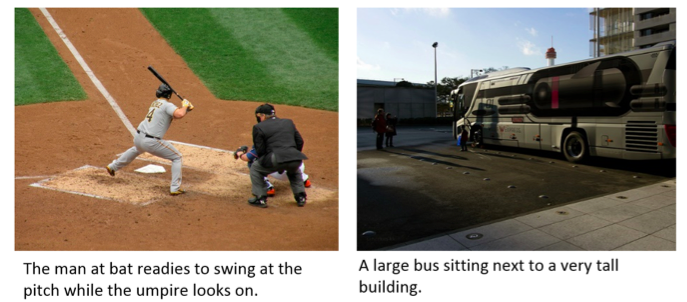
\includegraphics[scale=0.5]{images/ch5/captions-splash.jpg}
	\caption{Image caption examples. Source: \href{http://cocodataset.org/}{COCO Image Captioning Task}}
	\label{fig:caption-example}
\end{figure}


In the end we only used this dataset because the other common options are clearly outdated, such as the Flickr8K and Flickr30K. Although the latter was deemed as an interesting option for faster experiments in the first stages of the project, we finally upgraded the hardware with a very powerfull GPU that made it feasible to use the COCO dataset as the only experimental dataset, and still conduct a considerable number of experiments.

As a matter of fact, there is still a larger dataset supporting image captioning, the Conceptual Captions dataset, by Google  \citep{Sharma2018}, which also offers an online evaluation server and a \href{https://ai.google.com/research/ConceptualCaptions/leaderboard?active_tab=leaderboard}{public leaderboard}. However, it was released just a few months ago, and it is so huge, that it will probably take sometime before it is widely adopted by researchers\footnote{When I started this project there was no results yet but the ones published by google. A month later there are already four additional results from two different teams}.

For our project, we are using the images and the associated captions included in this dataset, which are divided in two separate sets: one for training, and another one for validation purposes.

\subsubsection{Training dataset}

This dataset includes a total of 82,783 unique images which are supposed to have 5 captions each, which would amount to 413,915 captions. However, in fact there are 414,113, probably because some image has more than 5 captions.

The length (number of words) of the captions is highly variable, with a maximum length of 51. The full corpus of text in the training captions dataset is 31,437.

After some initial analysis on the set of captions, we realized that a vast majority of captions are much sorter than the maximum lenght, therefore, for the sake of speeding up the processing of the recurrent layer, we decided to restrict the dataset to those captions having a maximum lenght of 15, which implied removing  13,370 images and 66,885 captions from the training dataset. This filter was applied before tokenizing the captions, thus in practice, when including the "<start>" and "<end>" tokens the maximum length of a sequence would be 17. Note the maximum length of the captions is actually a configurable parameter of the model (\lstinline{config.max_caption_length})

All in all, after filtering the dataset on a maximum caption length basis, we end up with a dataset containing 347,228 instances, each one consisting of a single caption and its associated image.

Concerning the vocabulary, the resulting corpus contains 24,775 words, which is still a huge number, considering than many words only appears once. Finally, we decided to set the vocabulary size to 10,000. The words excluded from the vocabulary were assigned the "<unk>" token. The size of the vocabulary is another hyperparameter of the model (\lstinline{config.vocabulary_size}).



\subsubsection{Validation dataset}

The full validation dataset contains 40504 images and  ???? captions. 
After applying the same filtering schema based on the maximum length of the captions, the dataset was reduced to 34043 images

Note that for the training process, each instance is made up of one single caption and its associated image, whilst for the evaluation process, each instance is an image and all its associated captions. 

\section{Experiments}

For the experiments we trained various models changing some hyperparameters:
\begin{itemize}
    \item The CNN: 'VGG16', 'incept', 'Xception, 'ResNet50', ,'InceptionResNet\_v2'
    \item The Type of units in RNN: 'GRU' or 'LSTM'
    \item The Embedding dimension: 256, 512
    \item The Number of recurrent units: 256, 512
    \item The Number of image features: 256, 512, 1024
    \item The Batchsize: 64, 128
\end{itemize}

We trained all the models for 30 epochs. In one case we trained the model for 90 epochs, but it was clearly overfitted, as 
Unfortunately, due to the long time required to train each model, we were unable to systematically try all the combinations of the chosen hyperparameters. 



\begin{table}[]
\caption{Evaluation results}
\label{tab:results}
\begin{tabular}{lllllllllllllll}
cnn & rnn & embed & state & feat & batch & optimizer & Bleu1 & Bleu2 & Bleu3 & Bleu4 & METEOR & ROUGE & CIDEr & attention \\
incept & lstm & 256 & 512 & 256 & 128 & Adam & 0.510 & 0.337 & 0.213 & 0.131 & 0.164 & 0.364 & 0.410 & False \\
incept & lstm & 256 & 512 & 256 & 64 & Adam & 0.521 & 0.342 & 0.215 & 0.132 & 0.166 & 0.367 & 0.406 & False \\
incept & lstm & 512 & 512 & 256 & 64 & Adam & 0.532 & 0.346 & 0.215 & 0.132 & 0.170 & 0.365 & 0.394 & False \\
incept & gru & 512 & 512 & 512 & 64 & Adam & 0.509 & 0.330 & 0.205 & 0.125 & 0.162 & 0.357 & 0.390 & False \\
incept & gru & 256 & 512 & 256 & 64 & Adam & 0.503 & 0.329 & 0.206 & 0.127 & 0.160 & 0.357 & 0.388 & False \\
incept & gru & 256 & 512 & 256 & 64 & Nadam & 0.515 & 0.336 & 0.209 & 0.127 & 0.163 & 0.360 & 0.380 & False \\
incept & lstm & 256 & 512 & 1024 & 128 & Adam & 0.509 & 0.327 & 0.201 & 0.121 & 0.162 & 0.355 & 0.370 & False \\
xception & gru & 256 & 512 & 256 & 64 & Adam & 0.507 & 0.326 & 0.199 & 0.120 & 0.160 & 0.352 & 0.365 & False \\
incept & gru & 512 & 1024 & 512 & 128 & Adam & 0.490 & 0.314 & 0.192 & 0.116 & 0.155 & 0.347 & 0.355 & False \\
resnet50 & lstm & 256 & 512 & 512 & 128 & Adam & 0.463 & 0.302 & 0.188 & 0.115 & 0.152 & 0.342 & 0.351 & False
\end{tabular}
\end{table}



% 90 epochs overfitting !!

% cnn = inception_v3
% rnn = lstm
% embedding_dim = 512
% rnn_units = 512
% num_features = 512
% weight_initialization = glorot_uniform
% batch_size = 64
% optimizer = Adam

% Final loss after 90 epochs 0.961689

% EPOCH 91 Loss 0.963 ... overfitting

% Bleu_1: 0.489
% Bleu_2: 0.311
% Bleu_3: 0.189
% Bleu_4: 0.113
% METEOR: 0.155
% ROUGE_L: 0.345
% CIDEr: 0.352
\chapter{Conclusions}
\label{ch:conclusions}

This chapter presents a critical self-opinion of the project and collects a number of potential improvements and future work.

\section{What I learned}

This project has supposed a huge advancement in my understanding of deep learning, especially in the fields of Natural Language Processing (NLP) and Computer Vision (CV). 

To begin with, I had to review a lot of literature on the topics of the project. Furthermore, being a project that combines NLP and CV, it covered a vast number of concepts, models and technologies. The initial stages of the project, where I was supposed to collect information on the project and review the state of the art, easily exceeded the expected effort by twice or tribble at least. One paper led to another paper, one model was soon discovered to have been surpassed by other models the following year, and so on. In the end, I expend more than a month actively researching the subjects, plus some extra days collecting and summarizing benchmark results from several, some times contradictory sources.

Secondly, I combined my research-oriented efforts with an intense self-learning program which basically took me through the 5 courses of the Deep Learning specialization program by \textit{deeplearning.ai} and professor Andrew Ng. at Coursera. Those courses gave me a wide and solid knowledge of deep learning, NLP and CV, combining both theory knowledge with hands-on experience, although the pace was probably too fast as to get a deep understanding of all the content: techniques to develop and improve deep networks, ConvNets, sequence, and recurrent networks, etc. There were many practical exercises, which were done using Python and Tensorflow on Jupyter Notebook. The case studies ranged from healthcare and autonomous driving to music generation, and natural language processing. All this knowledge was probably too much to digest in barely two months, but I still got a grasp of many of the concepts and techniques described in the courses, which was of great help to understand the research papers and model implementations I had to review as part of the project.

Third, I had to put into practice many of the concepts and techniques learned. These included fully connected layers, which I was already familiar with, but also ConvNets, RNNs, language modeling, seq2seq models, attention mechanisms, beam search, and so many other, most of which were new to me. In the beginning, started implementing quick prototypes as a proof of concept, to make sure my hardware had enough computational power to handle a big dataset, as was my intention. To that avail, I started prototyping by means of the Jupyter Notebook platform. Preliminary results made me buy a more powerful GPU, as described in \cref{sec:scope}. Soon, I jumped from the prototyping environment into a fully-fledged development environment, which  included the following tools and technologies:

\begin{itemize}
    \item Linux operating system, with CUDA drivers for GPU support
    \textit{Visual Studio Code} editor
    \item \textit{Git} control version and a remote \textit{GitLab} repository
    \item \textit{Conda} and \textit{Pip} for package management
    \item Tensorflow 2.0.0-alpha with GPU support, and Keras API.
\end{itemize}


\subsection{What I would have changed}

The development of a working system was an intense and very exciting experience too, but the entire development effort was highly conditioned from the very beginning by an excruciating lack of time. As a matter of fact, the analysis of the problem and the review of the literature consumed too much of my time, and thereafter I felt severely pushed by this lack of time, which made me commit several mistakes. 

\begin{itemize}
    \item First and probably the most severe mistake was developing and debugging the system using a big dataset. Once I realize I needed a smaller dataset for the initial development stage, I limited the number of examples actually used from the dataset, but as soon as I obtained an apparently working system I moved into the full dataset. By doing this, I had to expend a lot of time waiting for results rather than tweaking and improving the model.
    \item A second mistake that aggravated the former was the lack of a proper evaluation mechanism, which was delayed until the latest stages of the development process, when I included a tool to compute the usual metrics (Bleu, Meteor, etc.). Even worse, I didn't take the effort to interleave validation and training, that is, to check the generalization ability of the network as the training progressed. Too late I realized that the model was tremendously overfitting, as shown in the experimental section (\cref{ch:experiments}.
\end{itemize}

The combination of the two mistakes above made me waste a lot of time and computing resources overfitting the model far beyond the sweet spot. I couldn't imagine how soon overfitting started, but it was too late. However, this is a lesson I will never forget. 

\subsection{What I did not expect}

In general, the different experiments with the model performed considerably worse than expected considering the results achieved by the model it was inspired by, the one described in the "Show, attend and tell" paper by \citet{Xu2015}. However, but I have yet to find out whether this is due to implementation details, the lack of proper fine-tuning of the parameters, or a combination of the former.

The most frustrating result was due to the bad performance obtained by the beam search algorithm. It took several hours to develop a working \textit{beamsearch} algorithm. However, it was incredibly slow, and yet it obtained worse results than using greedy search, which was utterly unexpected. I should have to investigate this in the future since I am really disappointed.

After conducting a number of experiments with attention and still not getting as good results as expected, I decided to compare the model with attention against the same model without attention. For that purpose, I modified the existing model and conducted various experiments, but something was probably wrong because I couldn't obtain any reasonable results to compare against, but I did not have more time to debug it.

\section{Future work}

The limited time prevented me from adopting a more systematic and thorough approach to the development of a solution. In this final section I will enumerate some of the many things that could be done to complete, improve or extend the developed system, as well as alternative approaches to the image captioning problems, which include published work as well as some ideas that come to my mind based on what I have learned during this project.

First of all, some validation should be included as an integral part of the training process to monitor it and detect overfitting, perhaps combined with \textit{early stopping} as a form of regularization.

Second, given the results obtained, overfitting arises as one of the major problems with the model developed. Unfortunately, I realized very late the need for regularization mechanisms, such as \textit{batch normalization} and \textit{dropout}. This would be the most important improvements to undertake in the future, combined with the use of validation during the training procedure.

Third, it would be convenient to conduct more experiments, and in a more principled way, so as to have a proper distribution of values for the most important hyperparameters. It would be also very helpful to perform most of these experiments on a smaller dataset, such as the Flickr8K or the Flickr30K datasets, to get a more comprehensive understanding on the effects of the various hyperparameters and how to tune them before moving into larger datasets. 

Fourth, it would be nice to have a baseline to compare against, such as the same basic model without the attention mechanism. Actually, I tried to do this but something went wrong and I did not have time enough to debug it.

Finally, in addition to monitoring validation while training, it would also be very interesting to include some form of visualization, probably by means of the \textit{Tensorboard} visualization tool. This is something I did not have the opportunity to explore, but I would definitely add this as something to address in the future.

Besides the proposed improvements, there are a number of things that could be done in the future to extend the work done for this project.

\begin{itemize}
    \item To begin with, it would be nice to develop alternative models of attention to compare with, such as the global attention mechanism proposed by \citet{Luong2015} or a hierarchical attention mechanism as the one proposed by \citet{Khademi2018}.
    \item I'm really curious about the possibility of adding reinforcement learning to improve the captioning process, in the likes of the model proposed by \citet{Rennie2017}.
    \item Finally, aside from other forms of attention and alternative methods to generate captions, it would be nice to build an online application for demonstrative purposes. Since our model was developed in Tensorflow, it would be easy to load the model into a Web App by means of the \href{https://www.tensorflow.org/js}{Tensorflow.js} library.
\end{itemize}

\section{Concluding remarks}

All in all, retrospectively, I am very happy with having chosen this problem for my Master Thesis. It is a very challenging problem, and it was very exciting as a research problem. As a matter of fact, I ended up dedicating far more time than planned surveying the state of the art, but I did not regret this at all; it was quite inspiring to see so many advances in such a brief period of time.

However, I felt like I would have needed far more time to develop a more satisfactory system. In the end, the results were not up to my expectations, and I am looking forward to improving and extending it in my free time in the near future.

The code for the project


% bibliografia
\addcontentsline{toc}{chapter}{Bibliography}
\bibliographystyle{apalike}
\bibliography{references}

\end{document}